\subsection{31.07.2012 Die letzten Vorbereitungen}
Da unsere nördlichen Nachbarn mit der Lieferung von sehnlichst erwarteten Ersatzteilen in Verzug waren, musste unser Notnagel Tobi einspringen.
Zuverlässig wie eh und je konnte ich am Abend die benötigten Teile abholen.
Das Ganze noch Kurz im Bus eingebaut und der langen Fahrt sollte nichts mehr im Wege stehen.
Die Batterie, welche in letzter Zeit eher mit schwacher Leistung geglänzt hatte, konnte dank Garantie problemlos eingetauscht werden. (Danke Chantal)

\subsection{01.08.2012 Nutzlast?}
Der Tag stand ganz im Zeichen der Nahrungsaufnahme.
Der aufmerksame Beobachter könnte meinen, dass wir unsere Körpereigenen Reserven für unsere Reise aufladen.
Jedoch war der Grund nicht die Angst vor einer drohenden Hungersnot, sonder der 1.August, Nationalfeiertag der Schweiz.
Also reingehauen, kann ja nicht schaden.
Trotzdem mussten die anstehenden Arbeiten noch erledigen werden.
Das Tanken kurz nach dem traditionellen Feuerwerk in Baden bescherte der Coop-Tankstelle einen fetten Benzinflecken.
Mein Übermut und meine Viel hilft viel Philosophie wurde bestraft.
Der Übergang von Tankstutzen zu Benzintank präsentiert sich leicht spröde und der wertvolle Saft fand den Weg aus dem Bus zurück zur Tankstelle.
Glücklicherweise befindet sich das Leck in naher Distanz zum Tankdeckel.
So kam es, dass wir erst nach 11 Uhr unser wohlverdienter Schönheitsschlaf beginnen konnten.
Schon arg nahe am unschönen Weckerton, welcher uns um 04:30 für den Beginn der Reise aus den Federn holen sollte. 
Als erstes Ziel wollten wir möglichst viele Kilometer hinter uns bringen, damit wir nicht jeden Tag Auto fahren müssen.
Unser zugegebenermaßen ambitiöse Ziel war: Rom.
Viele Wege führen nach Rom, doch wir werden nur einen benötigen.
Viele selbsternannte Kritiker und Möchtegern VW-Bus Kenner lächelten über unser Vorhaben und streuten gezielt Zweifel.
Auch wir waren nach den jüngsten Ereignissen nicht abgeneigt den alljährlichen TCS Beitrag zu bezahlen um für das allerschlimmste gewappnet zu sein.  

\begin{figure}[hbt]
    \centering
    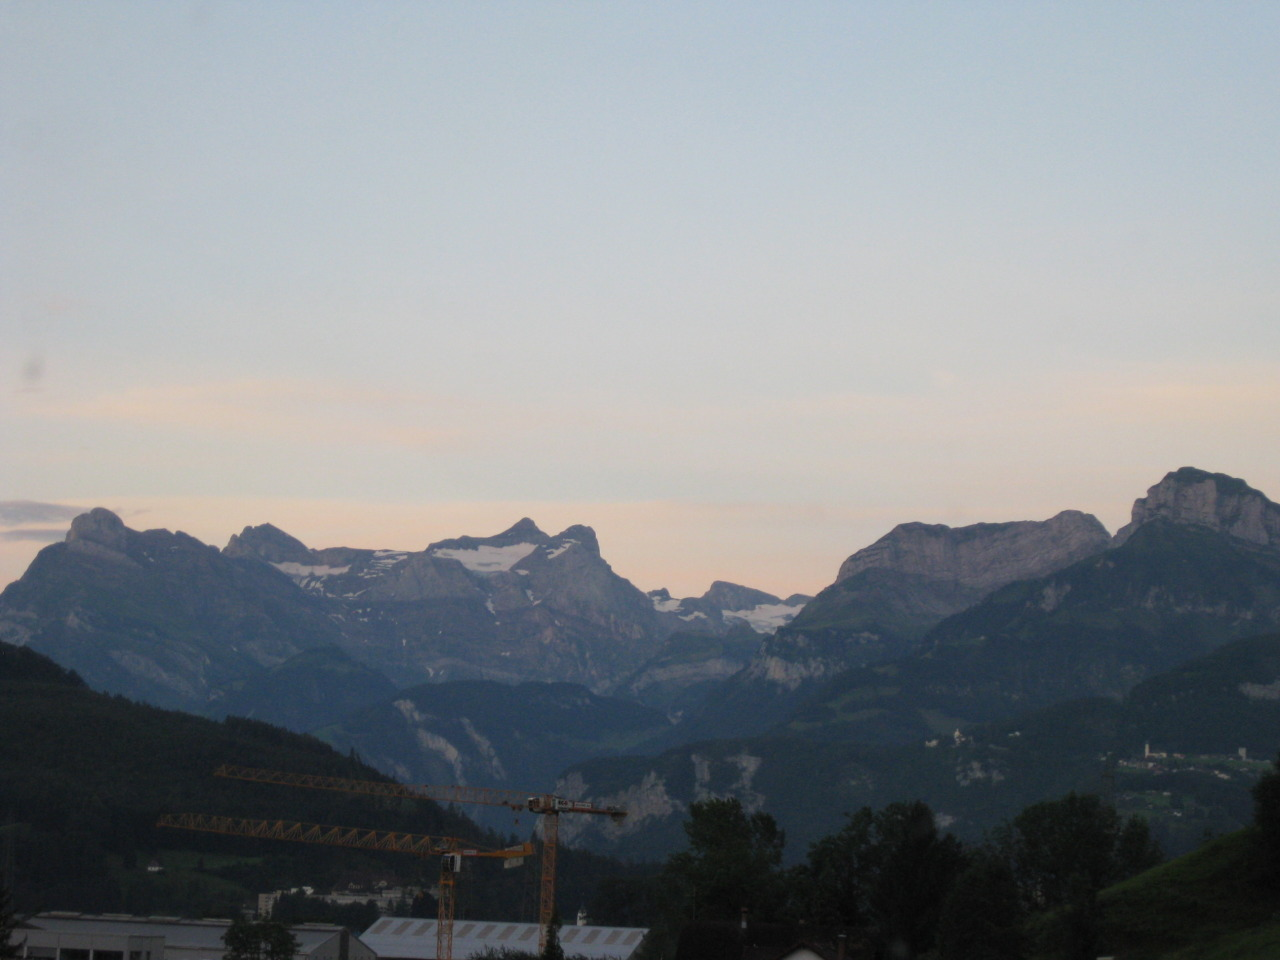
\includegraphics[width=\textwidth]{../Bilder/Sommer2012/1.jpg}
    \caption{Auf dem Weg in den Süden}
    \label{img:Sommer1}
\end{figure}

\subsection{02.08.2012 Es geht los}
Kurz nach 5 Uhr waren auch die letzten Ausreden, welche gegen eine Abfahrt gesprochen hätten aus dem Weg geräumt und wir machten uns auf den Weg gen Süden.
Schon früh fanden wir einen geeigneten LKW um uns in den Windschatten zu hängen und die Reise bei einem geringerem Lärmpegel zu absolvieren.
Der Berufsverkehr hielt sich in Grenzen und schon bald konnten wir unseren ersten Espresso an der Raststätte Gottardo Sud genießen.
Kurz nach der ersten Pause wurde die Frage nach dem Fackel für die Fährüberfahrt nach Kroatien leider negativ beantwortet.
Eine wilde Suche nach dem Bestätigungsmail auf dem Handy begann.
Wir entschlossen uns die nächste Raststätte zu nutzen um mittels Laptop nach dem vermeintlich verloren gegangenen Mail zu suchen.
Die Suche führte zu einem Treffer im SPAM Ordner, welcher einen Tag später automatisch gelöscht worden wäre.
Glück gehabt. Weiter ging die Reise Richtung Italienischer Grenze.

Da Jack mittlerweile zum Liebling der Polizeikontrollen avanciert ist (Sind daran möglicherweise die grünen Hibiskusblüten schuld?), waren wir auf den Grenzübertritt gespannt.
Doch ganz im Stile echter Italienischer Staatsangestellten verbrachten die anwesenden Zöllner ihre Zeit lieber mit Spässe als mit Kontrollen.

Nach einer kurzen Phase der Verkehrsüberlastung um Mailand ging die Flotte Reise Richtung Süden ungebremst weiter.
Die Landschaft wurde viel zu selten durch interessante Aussichten gestört.
Dominierend waren Felder und Hochspannungsmasten.
Waren zu Beginn die Temperaturen noch angenehm, näherte sich das Thermometer je länger je näher der Zone ziemlich bis wahnsinnig warm.
Man konnte Hühnchen fettarm zubereiten, wenn man sie aus dem offenen Fenster hält.
Gerade in Mitten einer LKW Kolonne, welche sehr häufig (zu häufig) auftraten, war der Atem eines Heissluftföhnes zu spüren.
Die lieben Lkws machten Chantal zu schaffen.
Gerade als sie den nötigen Schwung für ein Überholmanöver gesammelt hatte, scherte der schläfrige Chauffeur mit seinem langen Gefährt Richtung unserer Spur.
Dieses Manöver provozierte eine wahre Sammlung netter Ausdrücke, welche in ihrer Rohform so im öffentlichen Raum nicht abgedruckt werden sollten.

Endlich näherten wir uns Rom und damit begann die Suche nach einer Bleibe.
Die elektronische Sammlung von Campingplätzen um Rom schlug uns zwei Favoriten vor.
Um Überhaupt dort hin zu kommen mussten wir den Westring von Rom befahren, welcher uns mit Stau und den dazugehörigen spannenden Überholmanöver begrüßte.
Der erste Angesteuerte Campingplatz war closed.
So jedenfalls die Aussage eines beim Eingang abgestellten Typen.
Wir sollen es bei einem anderen Versuchen.
Das taten wir und wir hatten Glück.
200 Meter vom Strand entfernt fanden wir kurz vor 19:00 unser erster Standplatz.
Nach dem hastigen Einrichten stand einem Bad im Meer nichts mehr im Weg.

Auf dem Rückweg sahen wir ein schöne Restaurant am Meer, welches aber alles andere als gut besucht war.
Wir beschlossen, unser Glück nach dem Frischmachen dort zu suchen.
Natürlich war um 22:00 das lokal von Einheimischen überspült worden.
Ein kurzer Blick über die Strandpromenade bescherte uns Gewissheit, dass dieses Lokal das einzig brauchbare zu sein scheint.
Nur hier waren Autos geparkt.
So mussten wir uns mit dem Campingrestaurant begnügen.
Wir wurden keinesfalls Enttäuscht.
Chantal stellte die Spaghetti Pesto in Rekordzeit herunter und auch ich musste mich keinesfalls hinter der Pizza verstecken.
Die eigentlich ganz fleissige Bedienung musste jedoch genau in der Phase, in der die Mücken wieder ein prominentes Opfer gefunden haben, eine, nein zwei Rauchpausen einlegen.
Kurz vor 24:00 war der erste lange Tag unserer Reise Geschichte.

\begin{figure}[h]
   \centering
      %\subfloat[CAPTION]{BILDERCODE}\qquad
   \subfloat{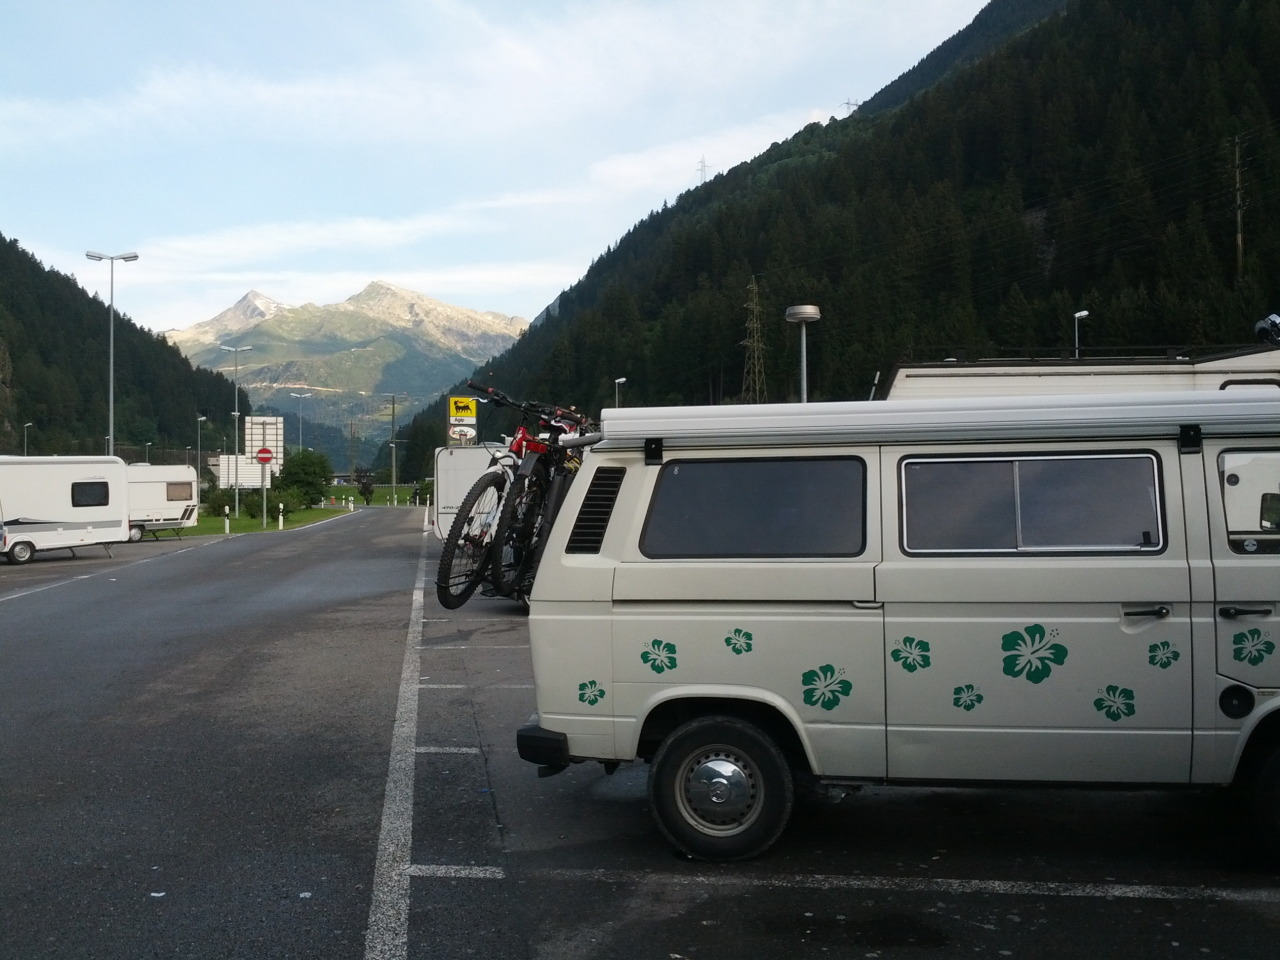
\includegraphics [width=0.3\textwidth]{../Bilder/Sommer2012/2.jpg}}\quad
   \subfloat{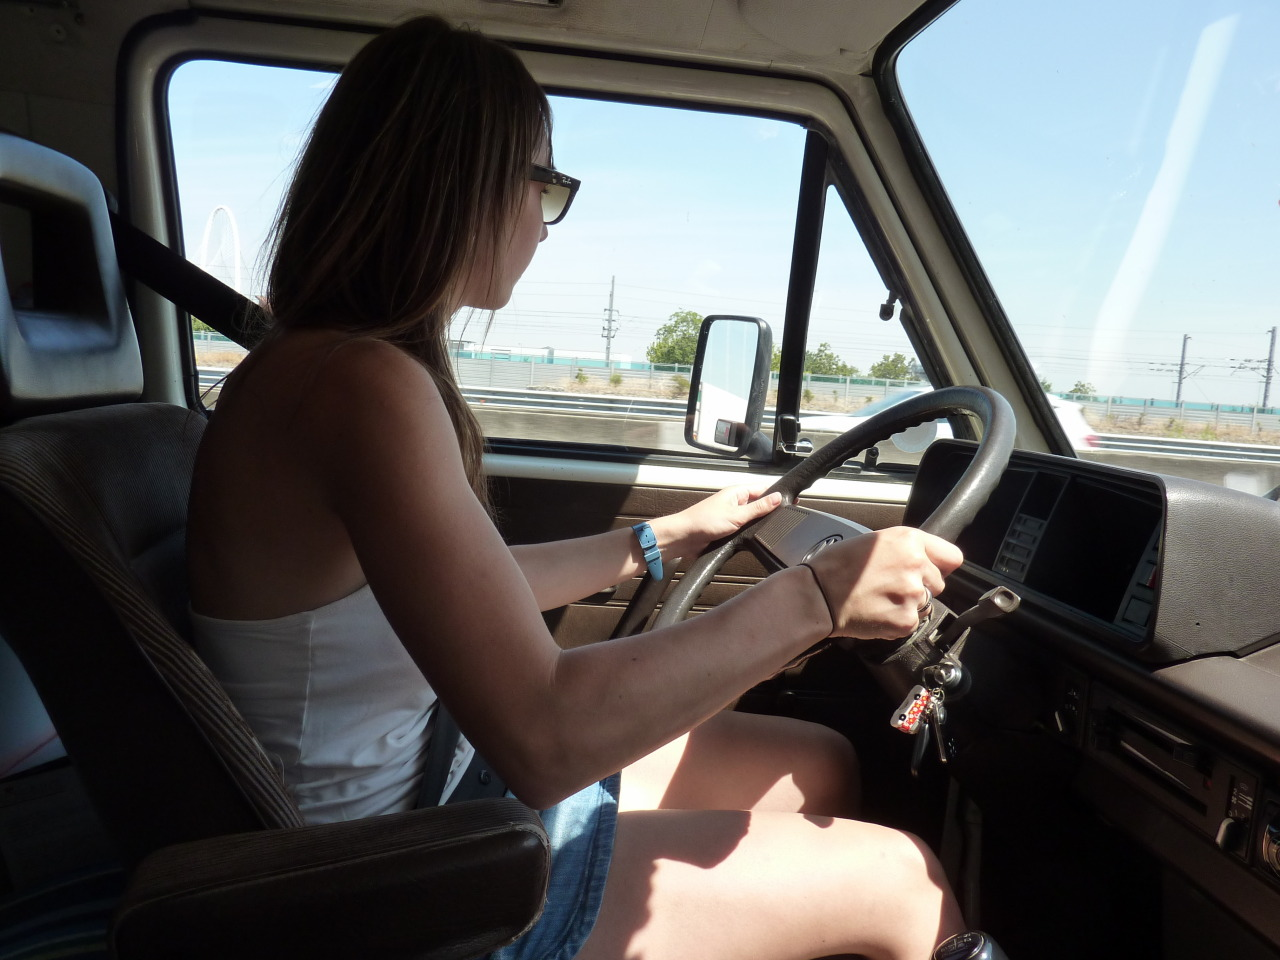
\includegraphics [width=0.3\textwidth]{../Bilder/Sommer2012/3.jpg}}\quad
   \subfloat{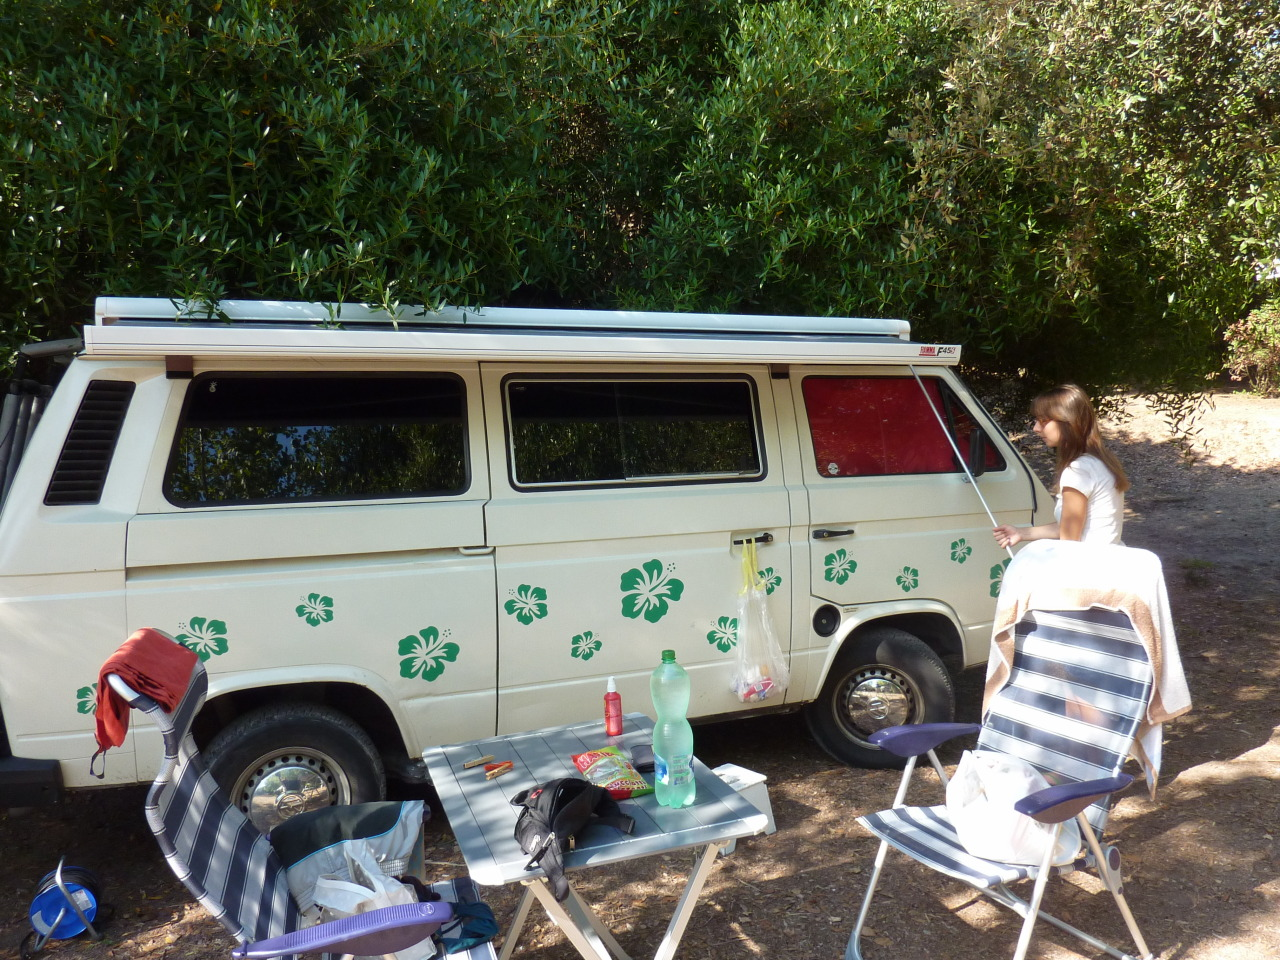
\includegraphics [width=0.3\textwidth]{../Bilder/Sommer2012/5.jpg}}\quad
   \caption[Weg und Ankunft in Rom]{Weg und Ankunft in Rom}
\end{figure}

\subsection{03.08.2012 Roma bei gefühlten 220° C}
Durch die geschickte Platzwahl konnten wir wunderbar im Schatten aufwachen.
Die Temperaturen waren auf ein angenehmes Mass gesunken während der Nacht.
Doch was bewegt sich da? AMEISEN.
Nicht gerade wenige nutzten unseren Bus als eine Art übergrosse Treppe um von einem Baum auf den Boden zu kommen.
Bei dieser Gelegenheit betrachteten diese Biester auch gerade noch unsere Innenraumaustattung.
Frechheit sowas.
Umparken war angesagt.
Mittels wilder Rangiermanöver ohne Rücksicht auf Flora und Fauna war der neue Standplatz inert Minutenfrist erreicht.
Anti-Brumm scheinen die vielbeinigen Plaggeister nicht zu mögen.
Jedenfalls veranstalten sie bei jedem Sprühangriff einen wilden Tanz und fallen wie Reife Pflaumen vom Bus.
Das Frühstück wurde trotzdem genossen.

Nach kurzer Recherche verwarfen wir die verwegene Idee Rom vom Campingplatz aus mit dem Velo zu erkunden.
Weit über 25 km Distanz und Aussicht auf einen eher warmen Tag machten uns diese Entscheidung leicht.
ÖV führt von hier bis ins Stadtzentrum und diese Transportmittel nutzen wir auch um in ca 1 Stunde neben dem Kolosseum aus dem Untergrund in der Hitze aufzutauchen.
Naja, so kolossal sah diese Ruine jetzt nicht gerade aus.
Auch das Forum Roman haute uns nicht aus den Socken oder ähm Sandalen.
Mit Römersandalen wollte ich durch das Forum Roman schlendern und die Latein-stunden der Bezirksschule wieder aufleben lassen: Ave Ceasar.
.Salve Titus.
.;) aber die Ruinen des Forums sahen gar nicht einladend aus; sie glichen eher einem Friedhof als einer spektakulären und historischen Stätte.
So machten wir uns auf den Weg zu der spanischen Treppe, die bekannteste Treppe der Welt.
Aber wo war diese? Obwohl sie ziemlich gross ist, hatten wir Mühe sie zu orten.
Da die Geographin die Treppe neben dem Forum Roman vermutete, sie aber überhaupt nicht dort war, wurde aus jeder Treppe rings um das Forum Roman die spanische Treppe ;) So haben wir viele Treppen erklommen und uns immer gedacht: die ist aber nicht so imposant wie auf dem Bild.
Nach einigen Fehlversuche haben wir dann doch herausgefunden, dass wir auf der falschen Fährte sind und haben einen neuen Anlauf genommen.

\begin{figure}[h]
   \centering
      %\subfloat[CAPTION]{BILDERCODE}\qquad
   \subfloat{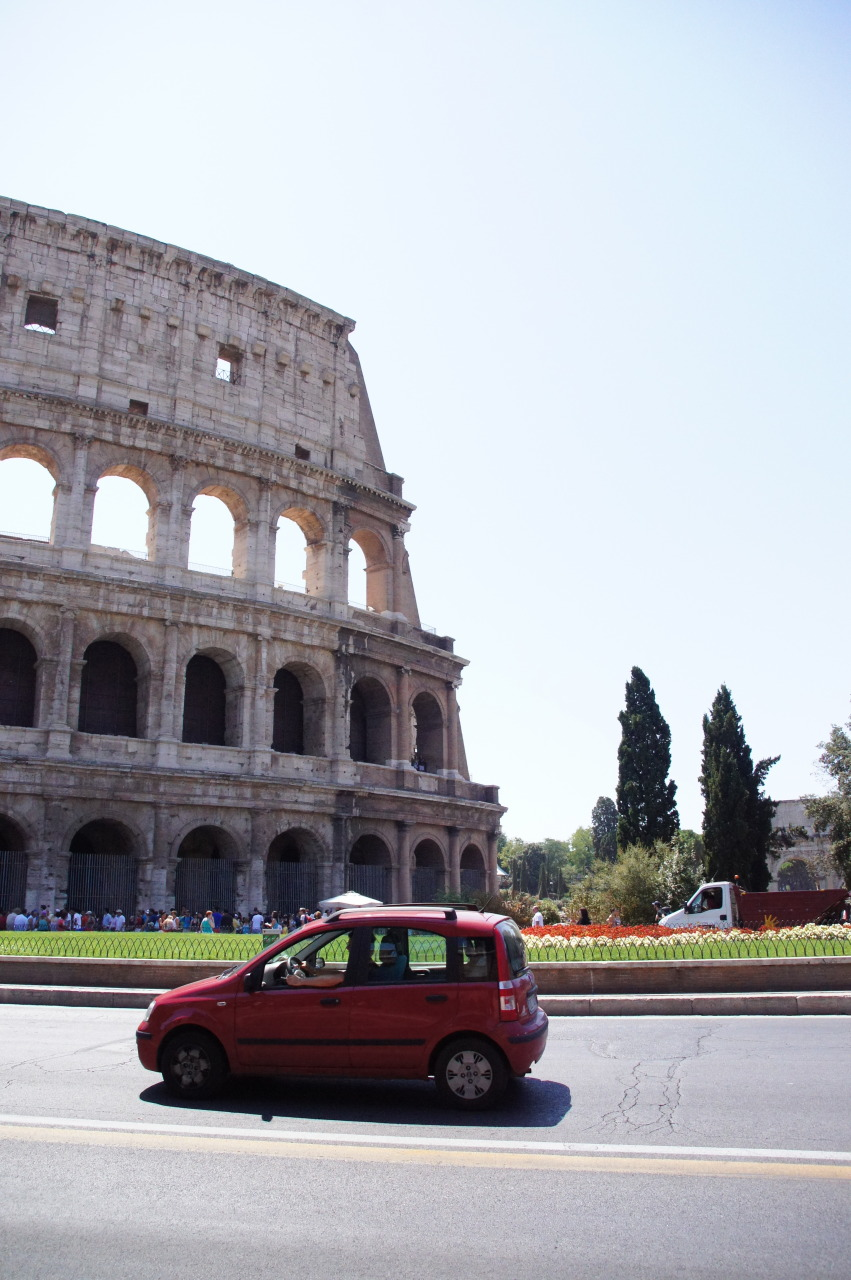
\includegraphics [width=0.3\textwidth]{../Bilder/Sommer2012/6.jpg}}\quad
   \subfloat{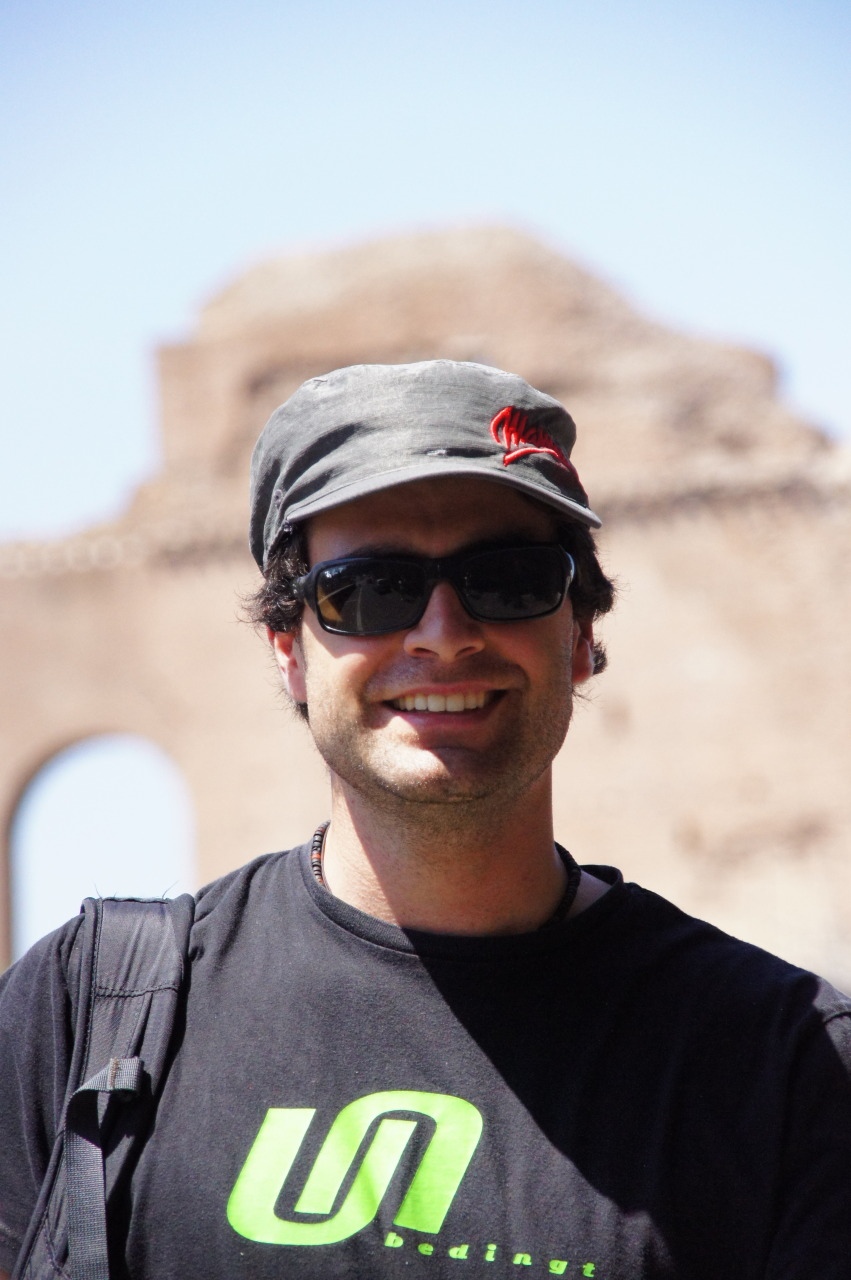
\includegraphics [width=0.3\textwidth]{../Bilder/Sommer2012/7.jpg}}\quad
   \subfloat{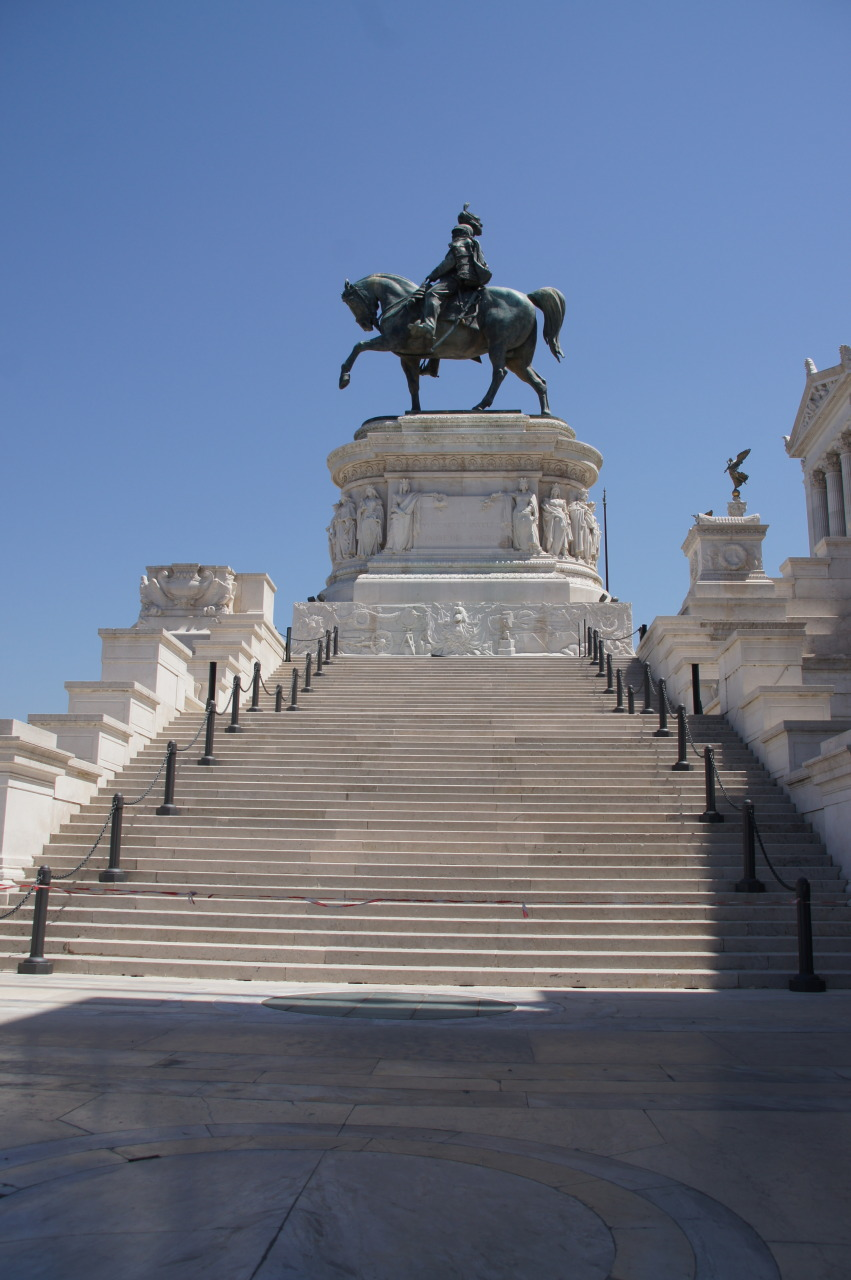
\includegraphics [width=0.3\textwidth]{../Bilder/Sommer2012/8.jpg}}\quad
   \caption[Sightseeing in Rom]{Sightseeing in Rom}
\end{figure}

Und da liefen wir direkt ins Judenviertel; jüdische Touristeninformation, Judensterne und koscher Essen gab es überall und das direkt neben dem Vatikan.
Sogar koscher Kebab gab es.
Dann meldete sich der Hunger.
Wir gönnten uns eine Pizza und Bruschetti, was aber eher eine schlechte Idee war.
Von der brennenden Sonne verging uns schnell der Hunger und wir kämpften um jeden Bissen.
Nur mit viel Wasser und Cola konnten wir fast alles herunterschlingen.
Die Konsequenz daraus war, dass unser Magen bei der Hitze das Essen nicht so gut ertrug und wir uns nach dem Essen schlechter fühlten als bevor.
Steff kämpfte mit der Hitze und der Pizza im Magen.
So marschierten wir zur spanischen Treppe, die wir schlussendlich auch fanden und welche immer noch nicht so spektakulär wie auf dem Bild im Reiseführer aussah.
Nach einem Drink (viiiiel Wasser;)) machten wir uns dann auch schon auf den Heimweg.
Wir mussten uns eingestehen, dass ein Stadtbesuch bei dieser Hitze nicht so angenehm ist.
Im Camping angekommen, freuten wir uns auf die Dusche und einen gemütlichen Abend.
Zum Nachtessen gab es feine Chilli-Oliven, Chips und Tomatensalat.
Mehr vertrug unser gestresste Magen nicht;) Wir lasen vertieft in unseren Büchern mit schöner Musik (Campingband) im Hintergrund.

\subsection{04.08.2012 Relaxxxxx}
Dieser Tag stand ganz im Zeichen des Faulenzen.
Wir schliefen aus und auch die aggressiven Ameisen konnten uns nicht früher aus den Federn holen.
Danach war ein Tag am Strand angesagt.
Mit Hilfe von Sonnenschirm und Wind konnte es man problemlos einen ganzen Tag am Strand aushalten.
Lesen und Faulenzen...
Am Abend besuchten wir das Restaurant am Strand, welches am ersten Tag hoffnungslos überlaufen war.
Dieses Mal reservierten wir jedoch.
Die Servierdüse konnte mir alles andrehen, jedenfalls sah das Chantal so und darum wurde aus dem Znacht ein gediegenes Mahl.
Erst spät am Abend kehrten wir zu unserem Bus zurück wo wir müde in Federn fallen wollten.
Jedoch machte uns ein hinterlistiges Sandkorn einen Strich durch die Rechnung.
Irgendwie verfing sich dieses Korn in einem Auge und blieb dort hartnäckig die ganze Nacht, was zu einer eher ungemütlichen Nacht führte

\begin{figure}[hbp]
    \centering
    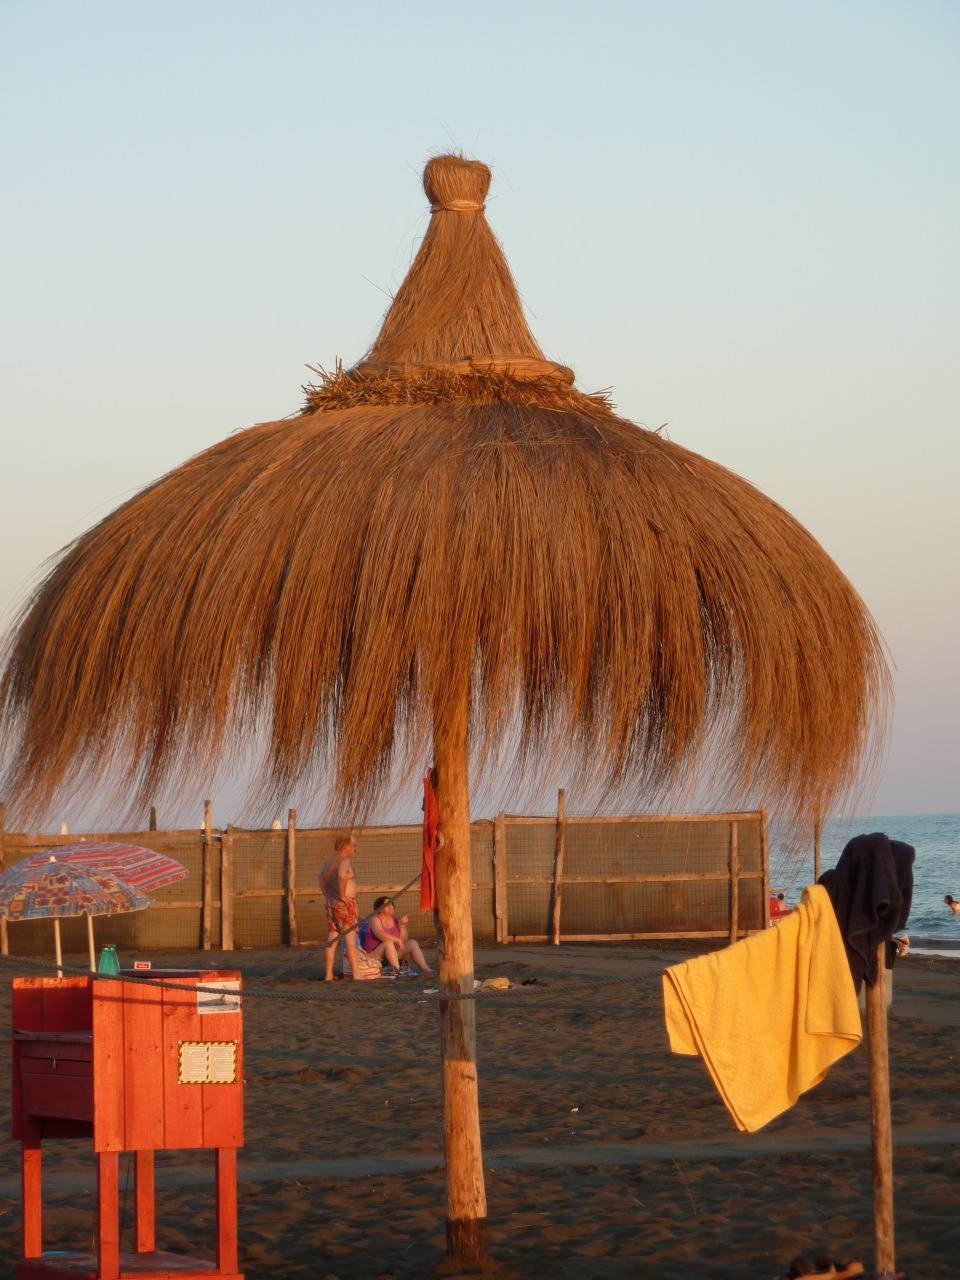
\includegraphics[width=\textwidth]{../Bilder/Sommer2012/4.jpg}
    \caption{Am Strand in Rom}
    \label{img:Sommer2}
\end{figure}

\subsection{05.08.2012 Je südlicher ,desto tsch tsch}
Der Morgen kam viel zu früh und beide Busfahrer hatten irgendwie einen komischen Magen.
So fiel das Frühstück sehr spärlich aus und schon bald fingen wir an unsere 7 Sachen im Bus zu verstauen.
Um 10 Uhr war Abfahrt und der Weg führte Richtung Vieste.
Es wurde zu einer äußerst ungemütlichen Fahrt, welche nur ein gutes Ende nahm, weil gewisse Tabletten aus Armeebestände den Weg in unsere Mägen fanden (Besten Dank dem Dr.  Sponsor).
Wir wollten die Fahrt schon aus gesundheitlichen Gründen unterbrechen, bissen uns dann aber bis nach Peschici durch.
Auch Jack musste das erste Mal so richtig leiden.
Die Temperatur blieb zwar stets im grünen Bereich, jedoch wollte er mit Hilfe des Standgases nicht mehr unbedingt seinen Dienst tun.
Unser neu montiertes Endrohr hing nur noch an einer Schraube statt an deren Drei.
Draht schafft hier Abhilfe (hoffentlich) Auch um 20:00 ist hier das Thermometer noch auf den oberen Etagen unterwegs und denkt nicht einmal daran in angenehmere Regionen zu sinken.
Das wird eine feucht-(fröhliche) Nacht.

\begin{figure}[H]
    \centering
    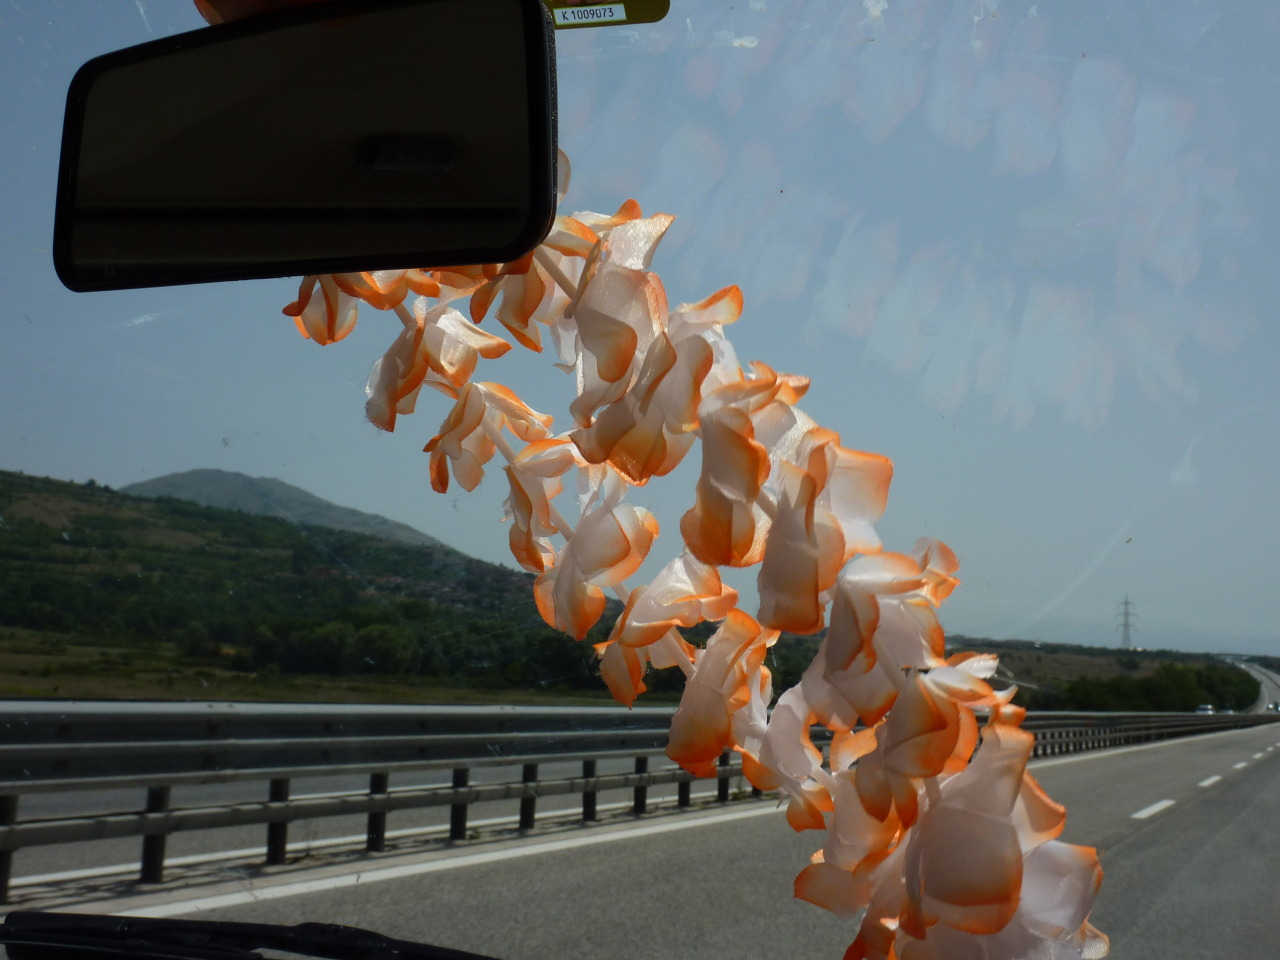
\includegraphics[width=\textwidth]{../Bilder/Sommer2012/11.jpg}
    \caption{Im Glutofen unterwegs}
    \label{img:Sommer3}
\end{figure}

\subsection{06.08.2012 Jack Sparrow alias Pepito}

\begin{wrapfigure}{R}{0.45\textwidth} 
  \begin{centering}
    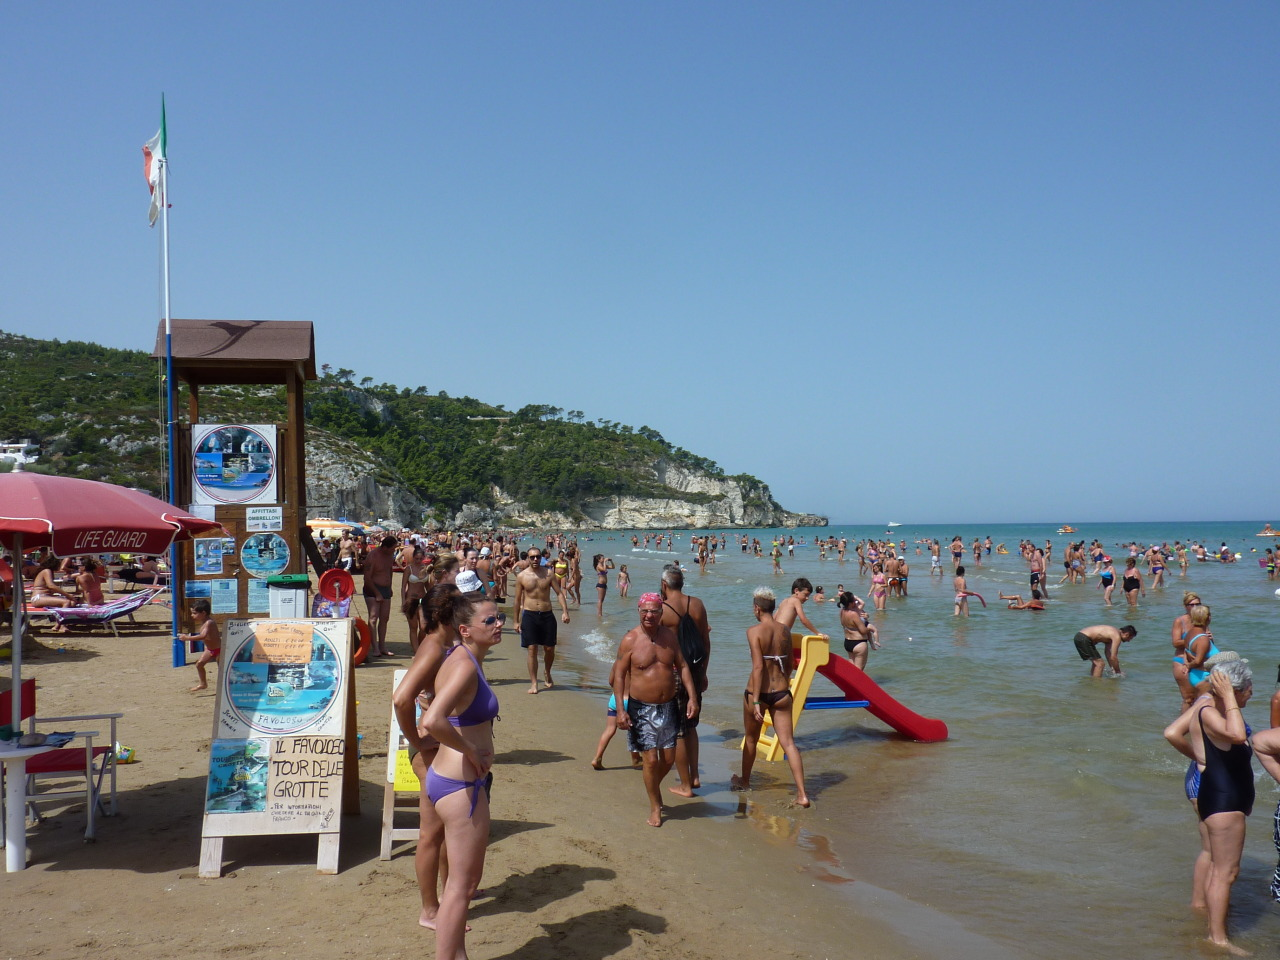
\includegraphics[width=0.4\textwidth, height=5cm, keepaspectratio]{../Bilder/Sommer2012/13.jpg}
    \caption{Action am Strand}
  \end{centering}
\end{wrapfigure} 

Die Nacht war trotz üblen Vorahnungen gar nicht so übel.
Chantal jubelte schon früh am Morgen darüber, dass ihr hartnäckiges Sandkorn verschwunden war.
So begann sie kurz nach 9 mit der Suche nach dem Mercato.
Wieso in aller Welt ist dieser Laden in der Höchstsaison geschlossen? Nach kurzer Absprache sattelten wir die Velos und begannen mit der Suche nach Nahrungsmittel.
Eine Tafel die mit äußerst optimistischen 20 Meter Distanz zum Supermercato wirbt wurde rasch gefunden so wie auch der Laden der 300 Meter von der Tafel entfernt war.
Das Frühstück fiel reichhaltig aus.
Das Ameisenproblem waren wir glücklicherweise los.
Trotzdem machte sich jedes Brotkorn das auf den Boden fiel sofort auf den Weg Richtung Nesteingang.
Die Ameisen hier sind mindestens doppelt so gross wie in Rom und Gott sei Dank nicht an der Inneneinrichtung interessiert.
Der Weg zum Strand war kurz und schon bald waren die Liegestühle in Beschlag genommen.
Doch was störte da mein sensibles Ohr? Gustavo Lima! Mindestens 50 Italiener in aller Form und Alter absolvierten eine Art Fitnesstraining am Strand.
Nach einer halben Stunde war Ruhe für ca.  10 Sekunden bevor der nächste Strandabschnitt mit anderen beknackten Spielchen anfing.
Schon bald begann ich mich auf die Suche nach ein wenig Ruhe und wurde schnell fündig.
Ein Typ, der Jack Sparrow alt aussehen lässt bot mir zwei Liegestühle an, welche auch sofort besetzt wurden, nach dem ich Chantal geholt habe.
Den Rest des Tages verbrachten wir mit Faulenzen und Baden.

Am Abend stand dagegen Fitness auf dem Speiseplan... Die Häuser schmiegen sich leicht erhöht an die Hügel und genau dort wollten wir mit dem Velo hin.
Um 21 Uhr waren die Temperaturen langsam erträglich und wir machten uns auf den Weg, welchen wir Schweissgetränkt zurücklegten.
Alle Läden hatten noch offen, dieser Umstand und die schönen, zahlreichen engen Gassen lösten Glücksgefühle bei Chantal aus.
Einen Teller Orechiette al Peschici führten bei mir zu einer ähnlichen Reaktion.
Die Abenteuerliche Abfahrt, welche wir im Schein der Stirnlampe unter die Räder nahmen war die letzte Aktion an diesem schönen Tag.

\subsection{07.08.2012 Slow down..take it easy}
Heute war wieder ein Strandtag angesagt.
Doch zuerst wollten wir nochmals das schöne Städtchen Peschici bei Tageslicht betrachten.
Um halb 9 Uhr machten wir uns mit dem Velo auf den Weg und hatten sogar noch Glück, da der Weg weit weit hinauf teilweise im Schatten lag.
Oben angekommen streiften wir gemütlich durch die herzigen Gassen und genossen die schöne Aussicht auf das türkisfarbene Meer.
Wir trafen sogar die Frau an, bei welcher ich gestern eine schöne Ledertasche geschenkt bekommen habe;) In einem Restaurant konnten wir einen feinen Kaffee geniessen, feine Croissant (eins mit Nutella;)) essen und sogar Flieger beobachten, welche im Meer Wasser für einen Brand hinter den Hügeln holte.
Da war einer seeehr glücklich über dieses Spektakel :D Dann fetzten wir mit den Velos den Hang hinunter, gingen in den Supermercato, wo wir einen Sonnenschrim fanden, machten einen Zwischenstop im Camping und schlenderten dann zum Strand (Bei dieser Hitze kann man nicht viel schneller laufen als zu schlendern) Am Strand versuchten wir unser frisch gekauften Sonnenschirm festzumachen, was sich aber eher als schwierig herausstellte.
Der Sand war ziemlich hart.
Nach kurzer Zeit kam uns eine Italienerin zur Hilfe und zeigte uns, wie man das macht.
Endlich konnten wir uns hinlegen, sonnen, lesen, faulenzen und baden.
Heute war es sogar aushaltbar an der Sonne (für einige;)), da ein angenehmer Wind wehte.
Den Abend verbrachten wir mit Trinken (Bier, Campari und Wein;)) und Essen.
Hmmm ich freue mich auf die Orechiette!  

\begin{figure}[h]
   \centering
      %\subfloat[CAPTION]{BILDERCODE}\qquad
   \subfloat{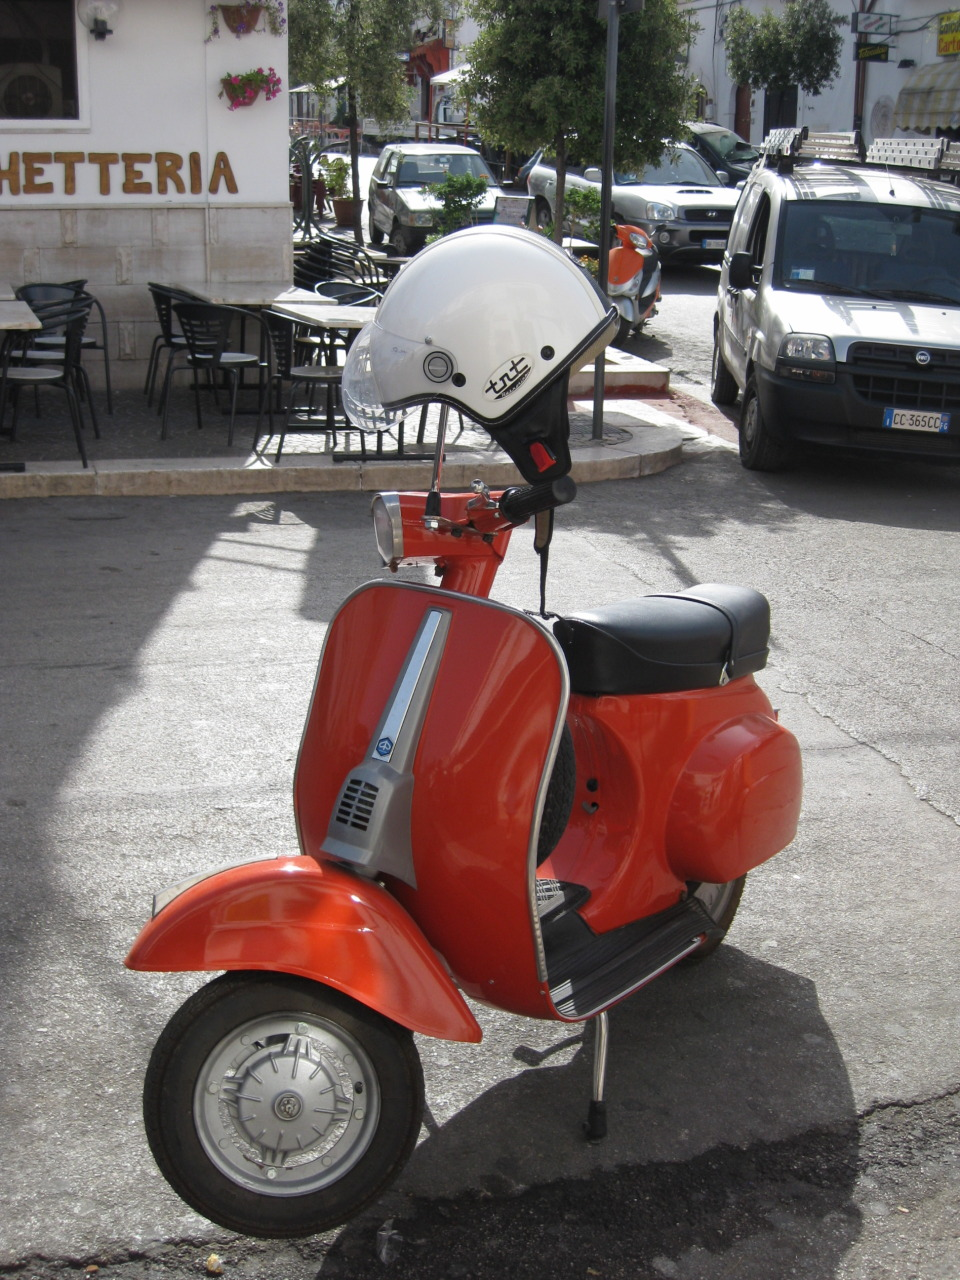
\includegraphics [width=0.3\textwidth]{../Bilder/Sommer2012/16.jpg}}\quad
   \subfloat{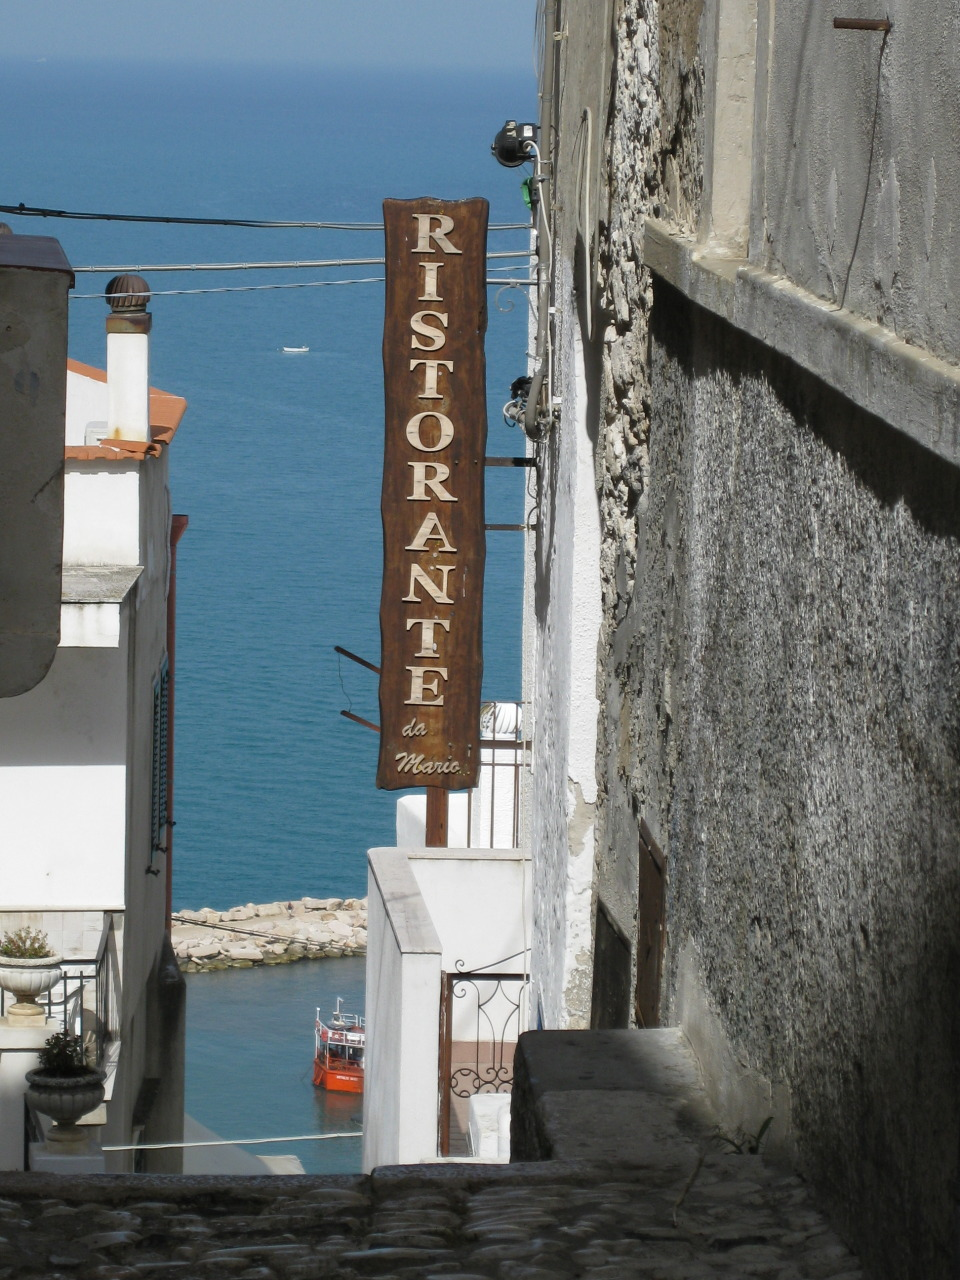
\includegraphics [width=0.3\textwidth]{../Bilder/Sommer2012/18.jpg}}\quad
   \subfloat{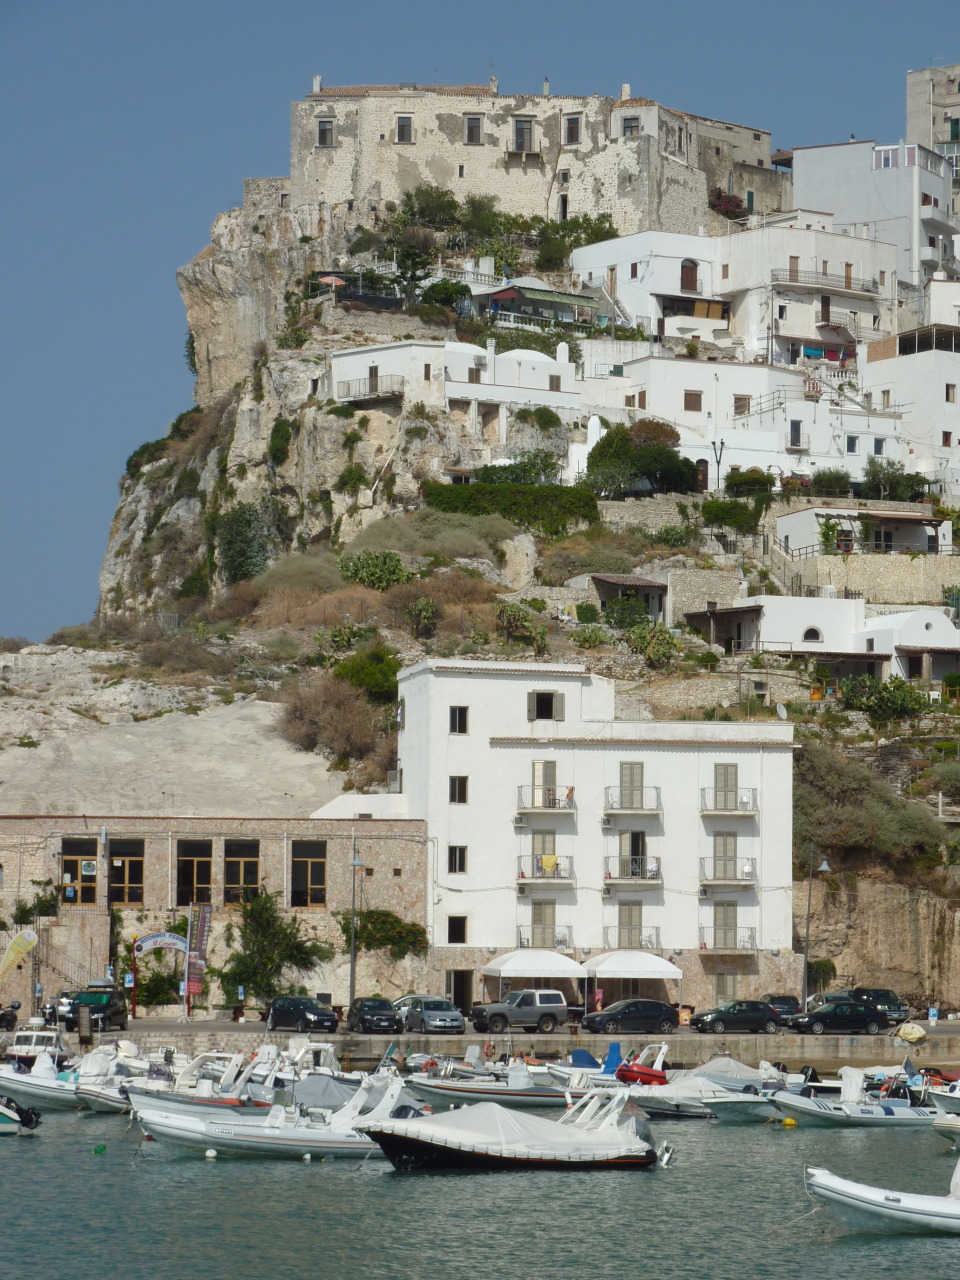
\includegraphics [width=0.3\textwidth]{../Bilder/Sommer2012/21.jpg}}\quad
   \caption[Peschici]{Peschici}
\end{figure}

\subsection{08.08.2012 Vieste}

\begin{wrapfigure}{L}{0.45\textwidth} 
  \begin{centering}
    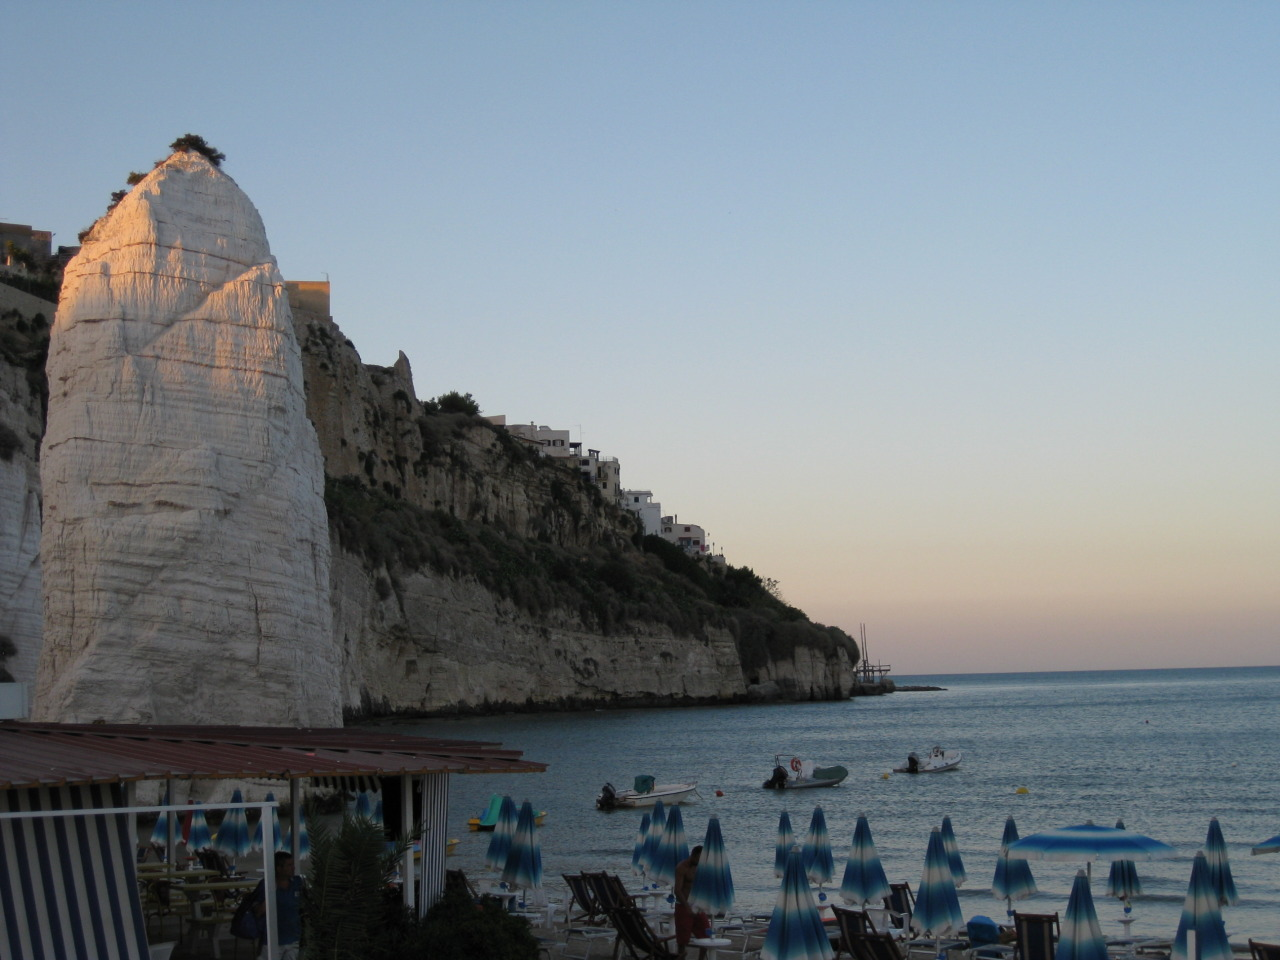
\includegraphics[width=0.4\textwidth, height=5cm, keepaspectratio]{../Bilder/Sommer2012/22.jpg}
    \caption{Vieste}
  \end{centering}
\end{wrapfigure} 

Um 12:00 mussten wir spätestens den Campingplatz verlassen haben.
Eigentlich kein Problem, wenn da nicht die sehr aktiv anstehenden Italiener wären.
Nur aus Mitleid der Bedienung kam ich an die Reihe.
Normalerweise schrie bei der Frage: "`Wer ist der nächste?"' immer eine als klassische Opernsängerin ausgebildete Italienerin aus der dritten Reihe und bekam ihre 2 Kilogramm Mortadella vor mir.
Beim Aufräumen fanden wir noch gewisse Überreste einer roten Flüssigkeit, die sich in alle Ritzen unseres Tisches eingenistet hat.
Böse Zungen behaupten es könnte dieselbe berauschende Flüssigkeit sein, welche zum umfallen des Weinglases verführte (gäll, Chantal :)) Nach dem Morgenessen waren unsere Habseligkeiten dann schnell verstaut und um 11:30 machten wir uns auf den Weg dem Meer entlang Richtung Vieste.
Das Navi war natürlich wieder äusserst optimistisch mit der Zeitangabe: 30 Min.
Die Fahrt war wunderschön und schon nach einer Stunde erreichten wir Vieste und den angepeilten Campingplatz.
Dieser war sich jedoch zu Schade uns für 2 Nächte aufzunehmen.
Absteigende müssen mindestens eine Woche dort bleiben.
Nicht mit mich.
Der nächste war dann schnell gefunden und bot zwar viel Schatten, dafür auch sehr wenig Platz.
Egal, hauptsache sofort an den Strand, an dem ich meine zugegebenermaßen abgeschauten Sonnenschirm Eingrabtechnik stolz den nicht anwesenden Badegäste präsentierte Badegäste.
Über die Mittagsstunden flüchten diese Weicheier und Beckenrandschwimmer immer zurück zu ihren klimatisierten Wohnungen und Wohnwägen.
Nur wir, sonnenverwöhnten Schweizer halten es am glühenden Strand aus.
Der Abend näherte sich immer mehr und meinen Versuch die Luftmatratze ohne Pumpe auf 2 Bar zu bringen scheiterten kläglich.
An dieser umgewandelter PET Flasche befanden sich extrem effiziente Ventile.
Luft geht nicht rein und auch nicht wieder raus.
Die 3 Liter die ich in mühsamer Arbeit in die Matratze gepresst hatte, konnte ich nun nicht wieder ablassen.

Endlich ging es Richtung Vieste.
Die ersten Schuhgeschäfte wurden durch Chantal geplündert, genauso wie Attila die westliche Welt heimsuchte.
Das Restaurant direkt am Meer sorgte für einige Kritik (meinerseits), trotz allem war es ein sehr gelungener Abend in einer äusserst schönen Stadt.
Bei der Ankunft auf dem Zeltplatz durften wir noch den Klängen sehr schlechter Karaokesänger lauschen, die fehlendes Talent geschickt mit Lautstärke zu kompensieren versuchten.
Die Sonne, die Wärme und ein wenig Campari sorgten jedoch für einen sehr tiefen und schnellen Schlaf trotz wildem Vibrieren von stark geölten Stimmbändern.

\begin{figure}[h]
   \centering
      %\subfloat[CAPTION]{BILDERCODE}\qquad
   \subfloat{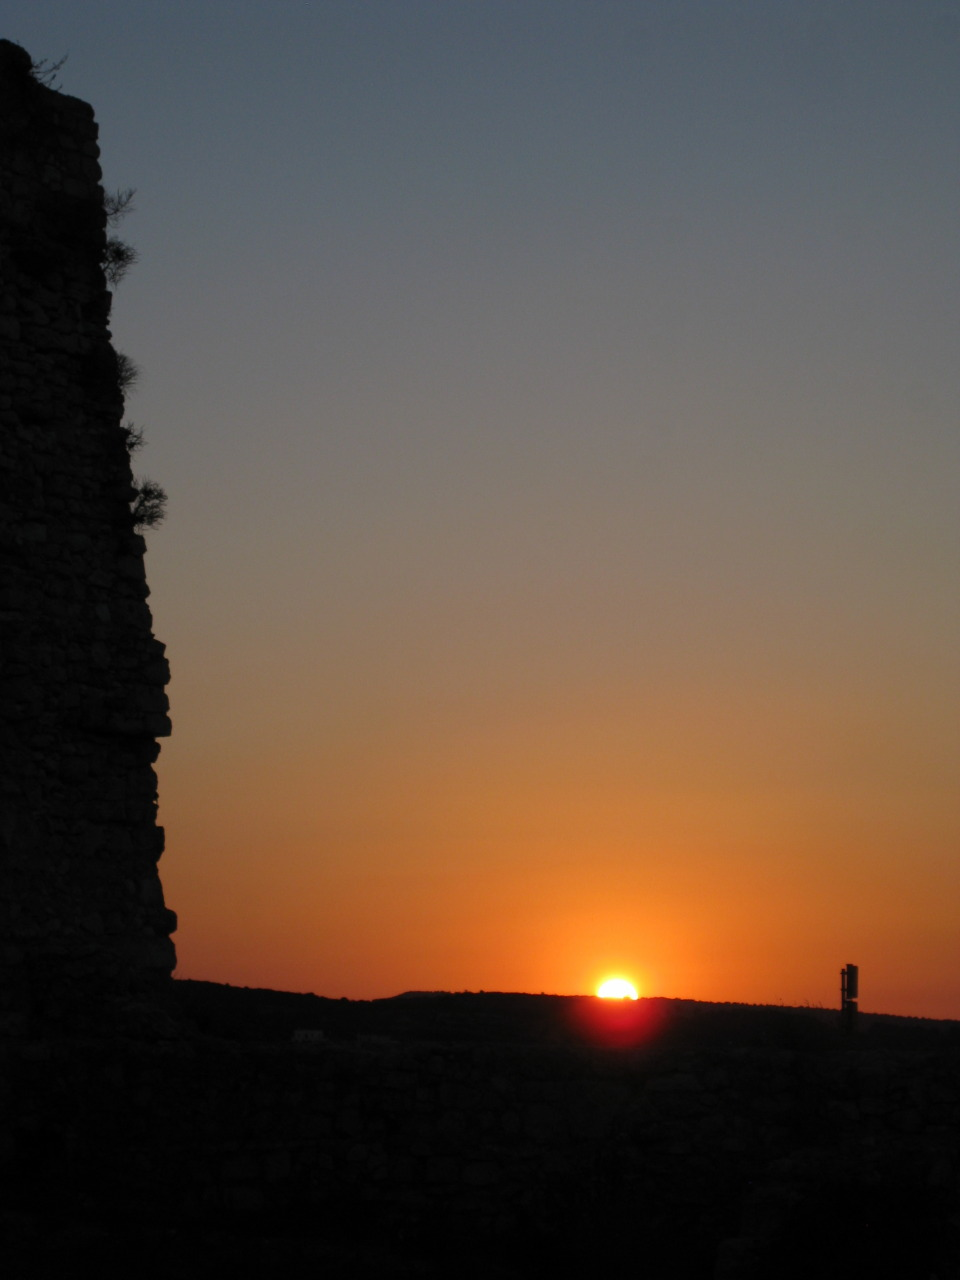
\includegraphics [width=0.3\textwidth]{../Bilder/Sommer2012/23.jpg}}\quad
   \subfloat{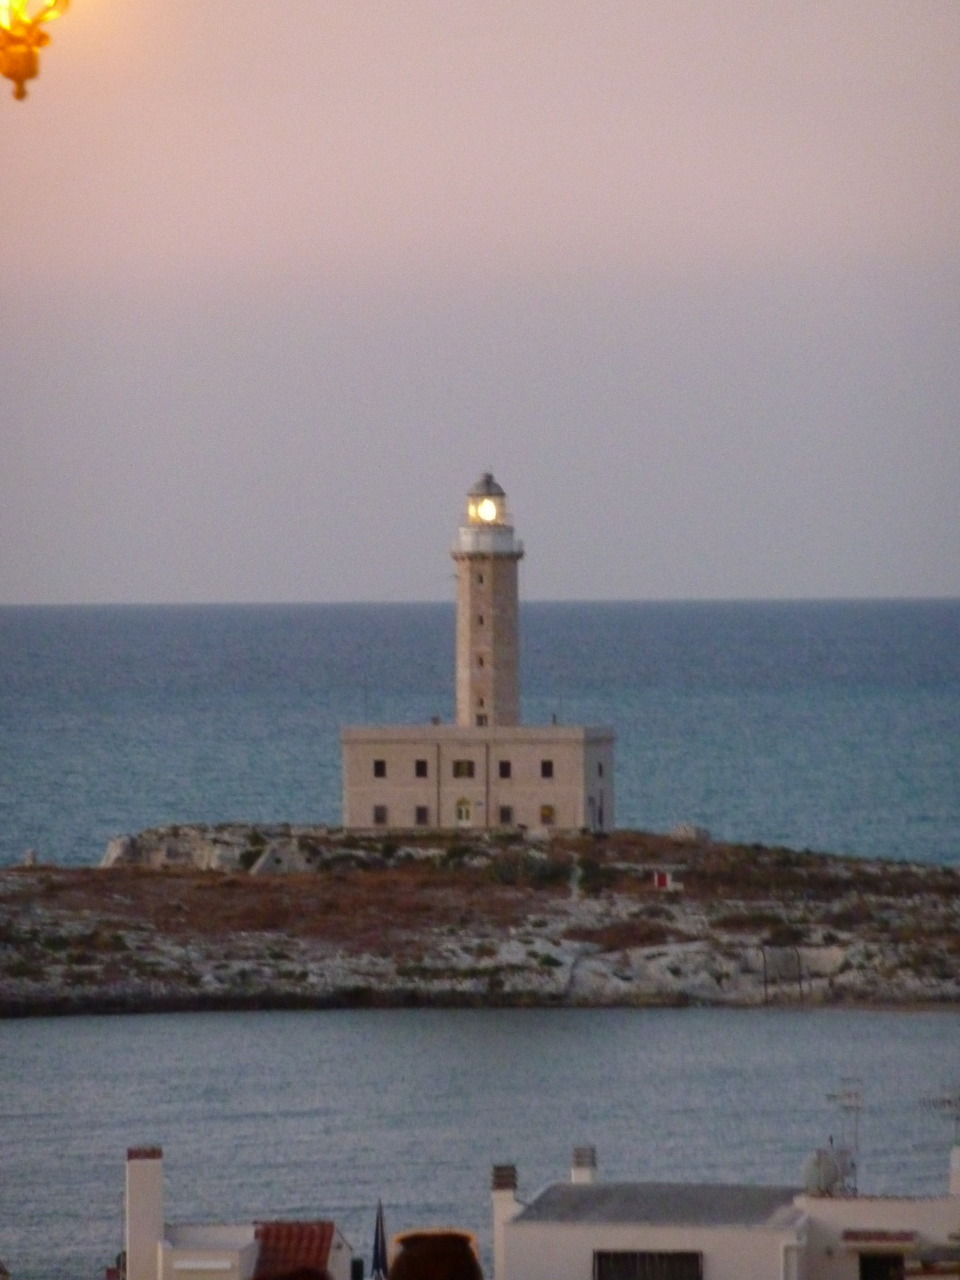
\includegraphics [width=0.3\textwidth]{../Bilder/Sommer2012/25.jpg}}\quad
   \subfloat{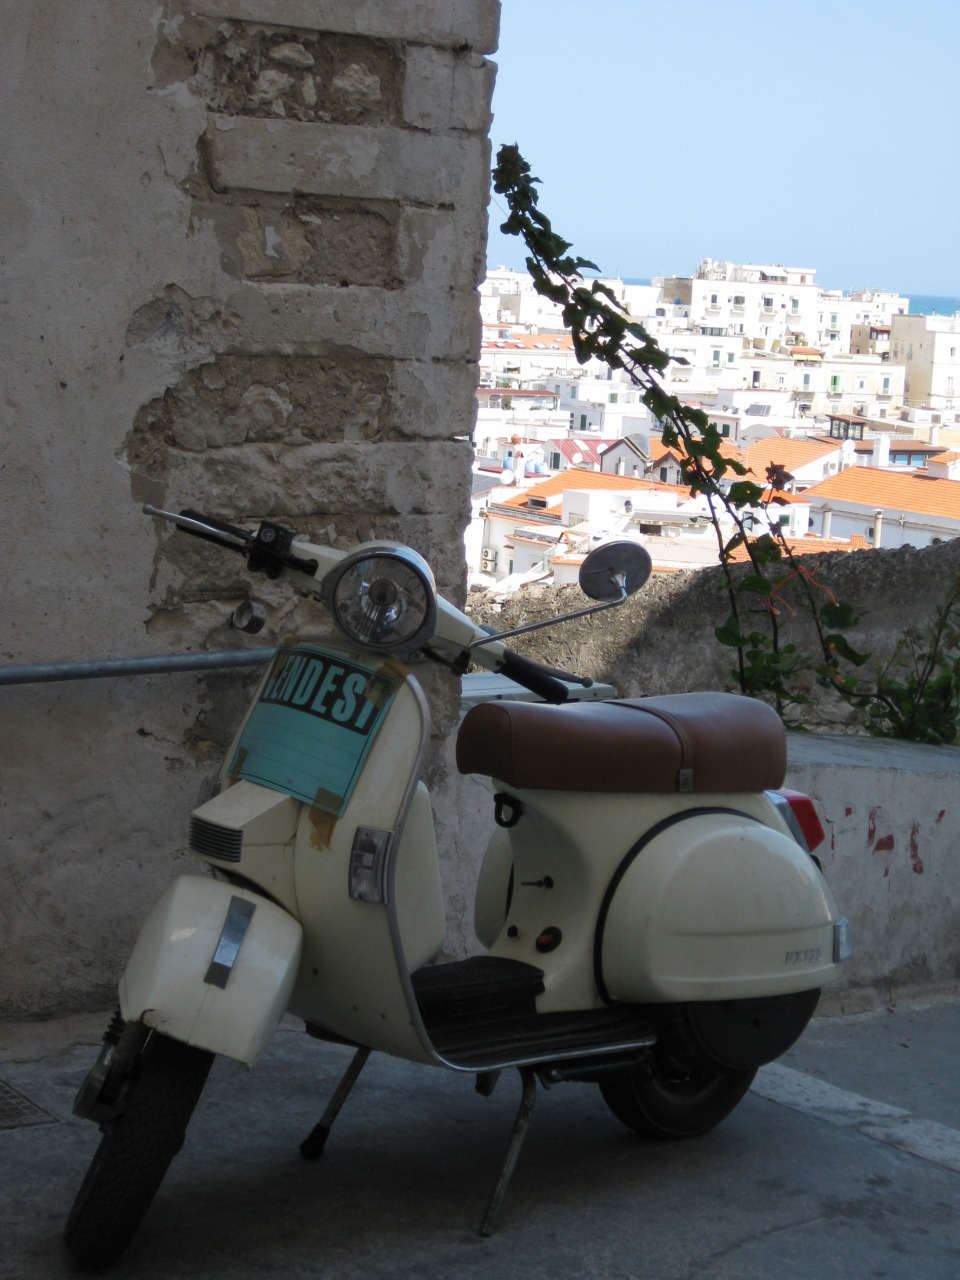
\includegraphics [width=0.3\textwidth]{../Bilder/Sommer2012/31.jpg}}\quad
   \caption[Rundgang durch Vieste]{Rundgang durch Vieste}
\end{figure}
 
\subsection{09.08.2012 Besuch der Altstadt}
Die weiteren Berichte werden sicherlich negativ beeinflusst von einem Ereignis, welches sich am 11.08.2012 ereignet hat.
Die folgenden zwei Tage waren garantiert lustiger und schöner als hier Beschrieben:
Ein weiteres Mal stiegen wir auf unsere Drahtesel und Radelten schon vor dem Mittag Richtung Vieste.
Dort angekommen starteten wir eine weitere Runde Sightseeing.
Viele Bilder wurden geschossen und von den nächsten Restaurierungsobjekten geträumt.
Den Kaffee nahmen wir bei einem Deutschsprechenden Italiener ein und genossen die Stadt bis in die Abendstunden.
Italienisch angehaucht suchten wir den Strand erst um 18:00 Uhr auf und genossen die angenehmen Abendstunden am Wasser.
Chantal konnte sich an der am Strand abgehaltenen Cha-Cha-Cha Tanzlektion kaum sattsehen.
Zurück auf dem nahegelegenen Camping bereiteten wir uns ein gemütliches Abendessen vor und fielen äusserts zufrieden auf die warmen Matrazen.

\begin{figure}[H]
    \centering
    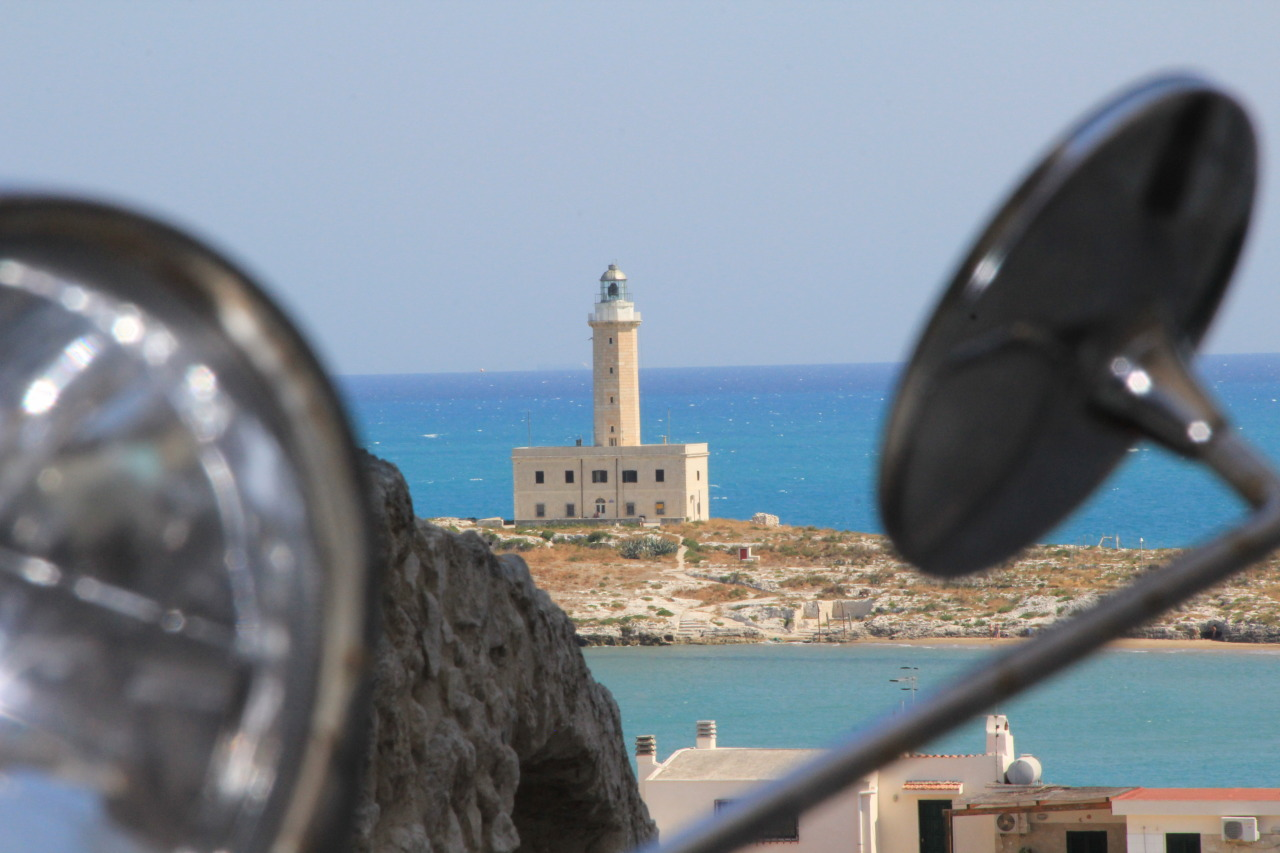
\includegraphics[width=\textwidth]{../Bilder/Sommer2012/30.jpg}
    \caption{Vespa in Vieste}
    \label{img:Sommer4}
\end{figure}

\subsection{10.08.2012 Fahrt nach Monopoli}
Auch hier mussten wir bis um 12:00 den Campingplatz verlassen haben.
Chantal besorgte das Morgenessen und ich verbrachte die Zeit mit der Vorbereitung für die Abfahrt.
Stolz verkündete ich nach getaner Arbeit eine neue Rekordzeit für die Aufräumarbeiten.
Schnell gezahtl und ab ginge es auf den wunderschön verschlungenen Küstenstraßen Richtung Süden.
Das nächste Ziel war Trani.
Das wir mit einem kurzen Umweg erreichten.
Ein Parkplatz war schnell gefunden und die Parkanlage am Hafen wusste mehr als zu überzeugen.

\begin{figure}[H]
   \centering
      %\subfloat[CAPTION]{BILDERCODE}\qquad
   \subfloat{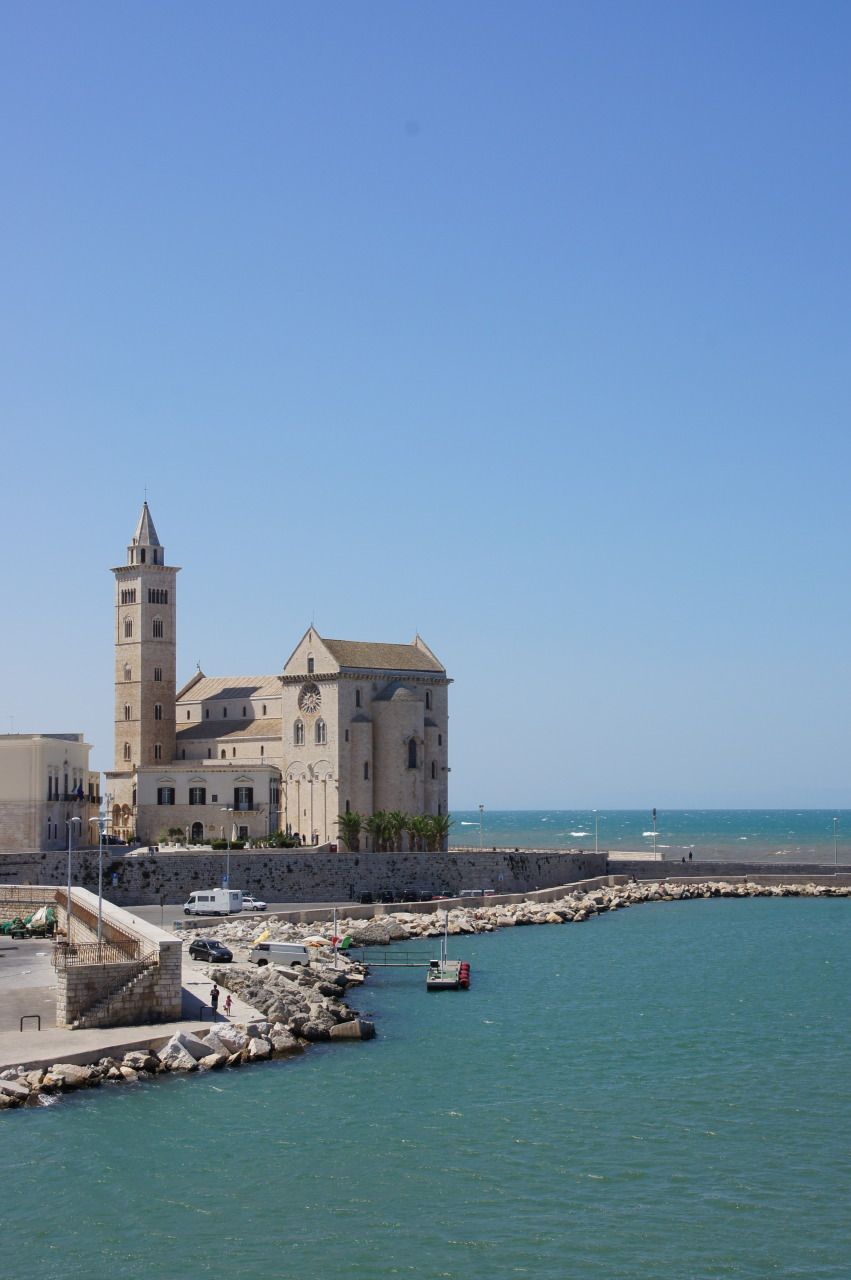
\includegraphics [width=0.3\textwidth]{../Bilder/Sommer2012/38.jpg}}\quad
   \subfloat{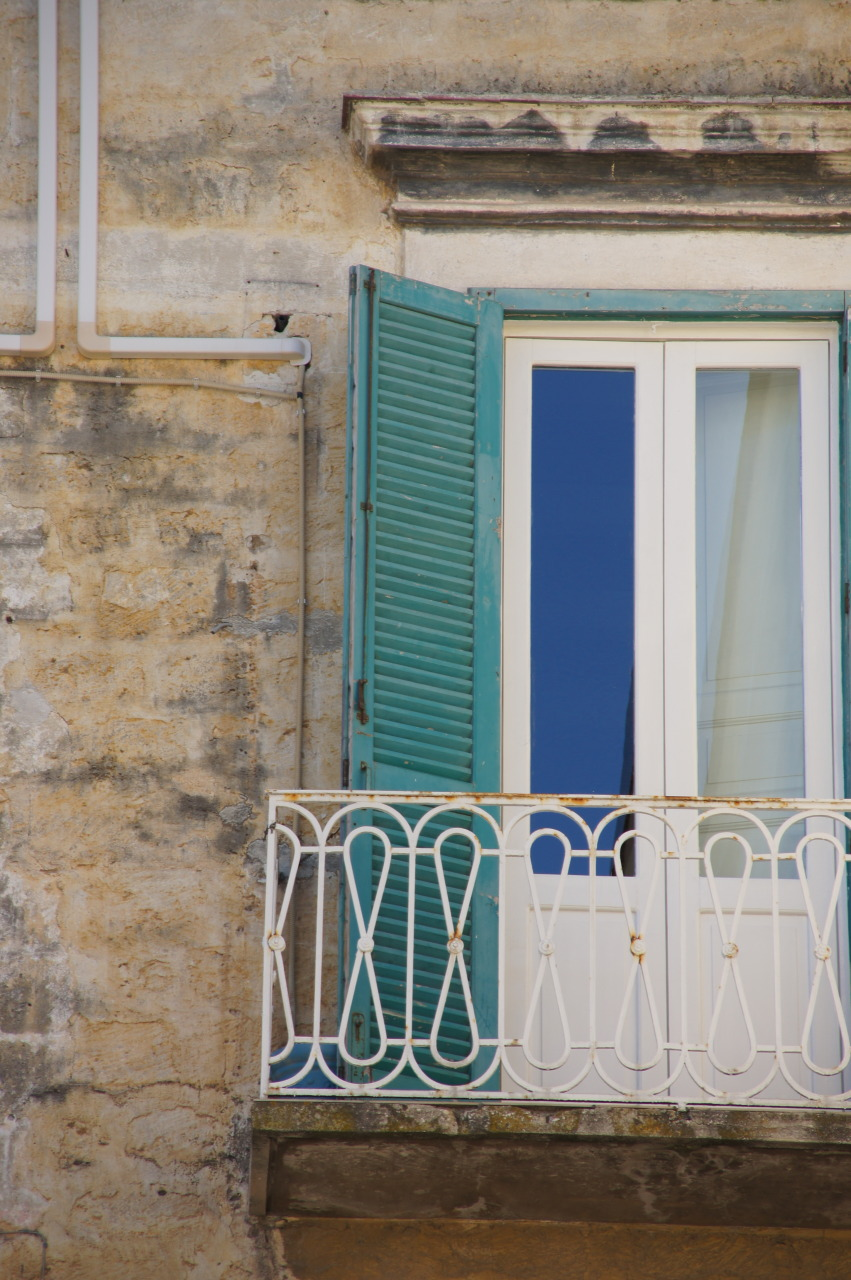
\includegraphics [width=0.3\textwidth]{../Bilder/Sommer2012/40.jpg}}\quad
   \subfloat{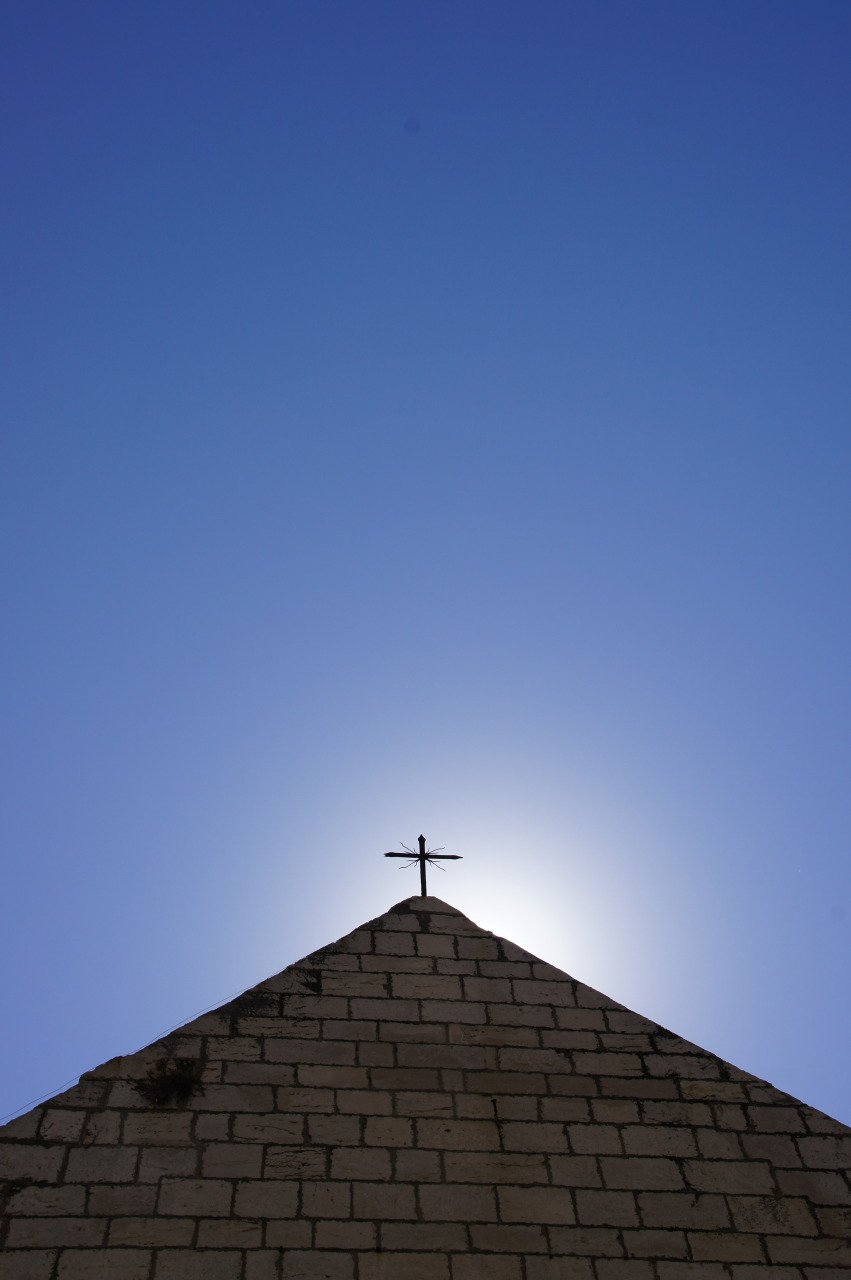
\includegraphics [width=0.3\textwidth]{../Bilder/Sommer2012/41.jpg}}\quad
   \caption[Trani]{Trani}
\end{figure}

Ganz im Gegenteil zur Altstadt.
Als Entschuldigung muss hier aufgeführt werden dass zwar Siesta war, trotzdem glich das ganze einer Geisterstadt.
Einzelne Touristen schlurften durch die Gassen, alles andere war leer.
Eine Bar, welche geöffnet hat war nicht auszumachen.
Schlussendlich nahm uns ein Restaurant auf, bei dem sich die Bedienung über unsere sehr begrenzte Bestellung wunderte.

\begin{figure}[H]
    \centering
    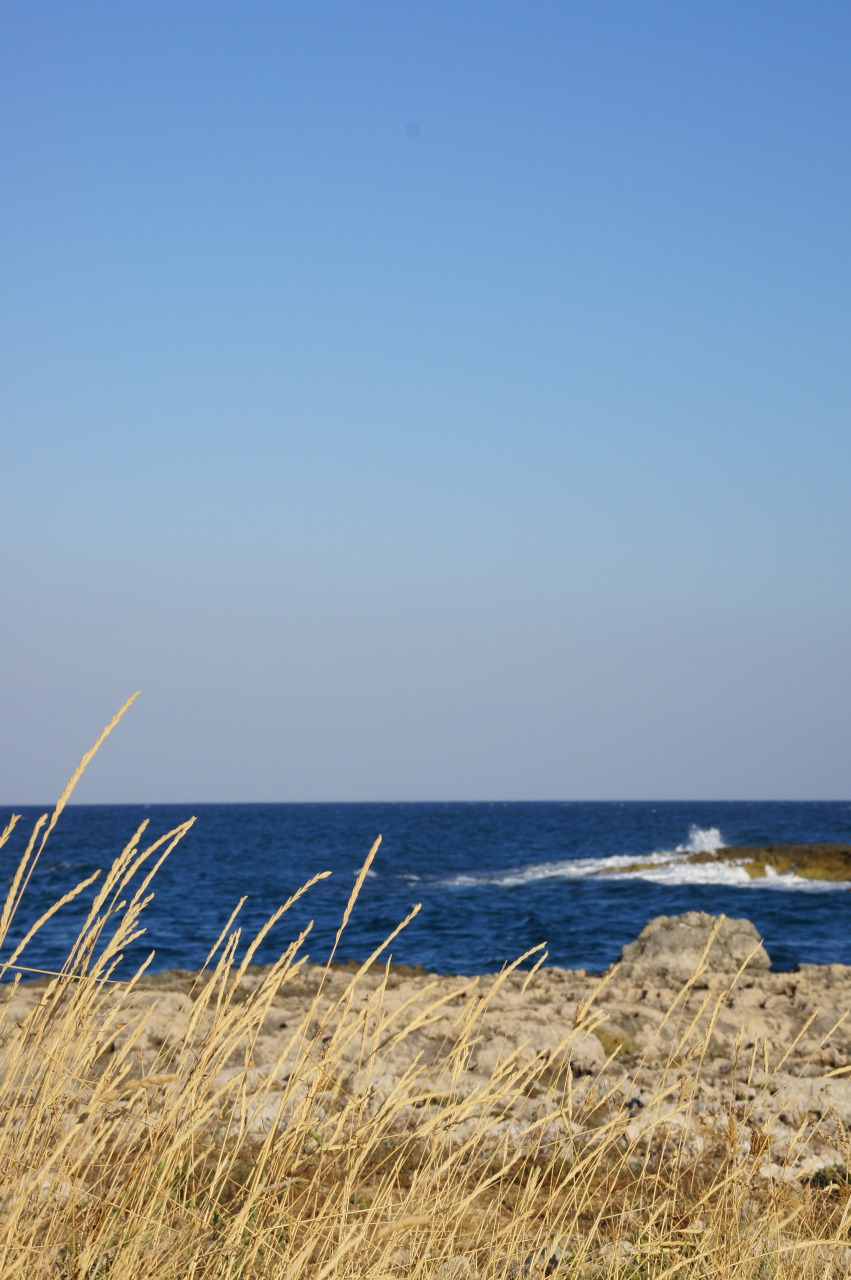
\includegraphics[width=0.5\textwidth]{../Bilder/Sommer2012/43.jpg}
    \caption{An der Küste bei Monopoli}
    \label{img:Sommer5}
\end{figure}

Nach dem der Bus wiedergefunden war, ging es weiter auf der SS 16 Richtung Bari/Brindisi.
Der Verkehr um Bari verhieß nichts positives für die baldige Wiederkehr am nächsten Dienstag.
Der Reiseführer versprach schon keine Anhäufung von Campingplätzen mehr und tatsächlich machten sich die begehrten Abstellplätze äußerst rar.
Bei einem ersten kurzen Besuch von Polignano al Mare konnten wir keinen Campingplatz ausfindig machen.
4 km südlich von Monopoli hatten wir dann mehr Glück.
San Stefano nahm uns in Empfang.
Die Einweisung auf den Platz nahm ein übereifriger Ciao fahrender Platzgehilfe vor.
Wie wurden in Mitten von Dauercamper platziert.
Als ich den Versuch unternahm Jack auf dem Platz zu wenden, kam er mit lautem Zweitaktgeknatter angebraust und wies uns wild fuchtelnd vermutlich auf irgendetwas hin.
Wir verstanden nur das wir den Bus wieder drehen mussten.
Jedoch reichte so unsere Kabelrolle nicht bis zur nächsten Elektrizität spendenden Pfosten.
Genau in diesem Augenblick durchzog es mich wie vom Blitz getroffen.
Ich hatte in Vieste den Adapter auf die lustigen Euro Stecker stecken gelassen.
SHIT, so viel zu der Bestzeit im Aufräumen.
Ohne Strom kein Kühlschrank, kein
... und so weiter.
Ich hätte mich schlagen können.
Der Besuch am Camping eigenen Strand besänftigte die Gemüter wieder.
Pläne für eine Neubeschaffung wurden gemacht und Routen für das Velo nach Monopoli verglichen.
Ab ging es.

Die Stadt war wunderschön von einer hellen Stadtmauer eingesäumt.
Schmuckgeschäfte lockten und schon bald trafen wir auf dem Hauptplatz ein um einen gemütlichen Apéro zu geniessen.
Noch schnell eine Flasche Wein gekauft und zurück ging es mit der Suche nach unseren Fahrrädern.
Die Fahrt verlief durch absolute Dunkelheit und nur unsere Stirnlampen und das Velolicht verhalfen uns zu einer eingeschränkten Sicht auf die Strasse.
Auf dem Campingplatz angekommen wehte uns ein starker Wind entgegen.
Keine Chance auf ein gemütliches Kochen vor dem Bus.
Also die "`Küche"' im Bus montiert und nach kurzer Zeit wurde das Abendessen serviert.
Noch kurz einen Film auf dem Laptop angeschaut und dann friedlich wurde friedlich eingedöst.

P.S. Der Wein blieb an diesem Abend unangetastet. Gerüchten zu Folge war der Apéro daran Schuld.

\subsection{11.08.2012 Wunderschöner Tag der am Abend leider eine sehr negative Wendung nahm.}
Das ist er also nun, unser Schicksalstag. 
Aber zuerst vorne Angefangen: Nach dem Morgenessen und dem Aufsuchen des Mercato (Eher eine Bar als ein Mercato... anyway) begaben wir uns ans Meer.
Leider war der Aufenthalt dort zeitlich begrenzt, da die augenscheinlich strenge Campingleitung mit Ciao-betriebenen Hilfssheriff, eine Fahrverbotszeitzone eingerichtet hat.
Ab 13:30 bis 16:00 war jeglicher Verkehr untersagt.
Jack machte schon bei den wilden Rangierversuchen mit seinem lockeren Auspuff auf sich aufmerksam und so versuchten wir wenn immer irgendwie möglich uns an die Spielregeln zu halten.
Am Strand war der Kindergarten los.
Chantal amüsierte sich königlich über das wilde Treiben.
Andere verließen fluchtartig den Tatort.

\begin{wrapfigure}{L}{0.45\textwidth} 
  \begin{centering}
    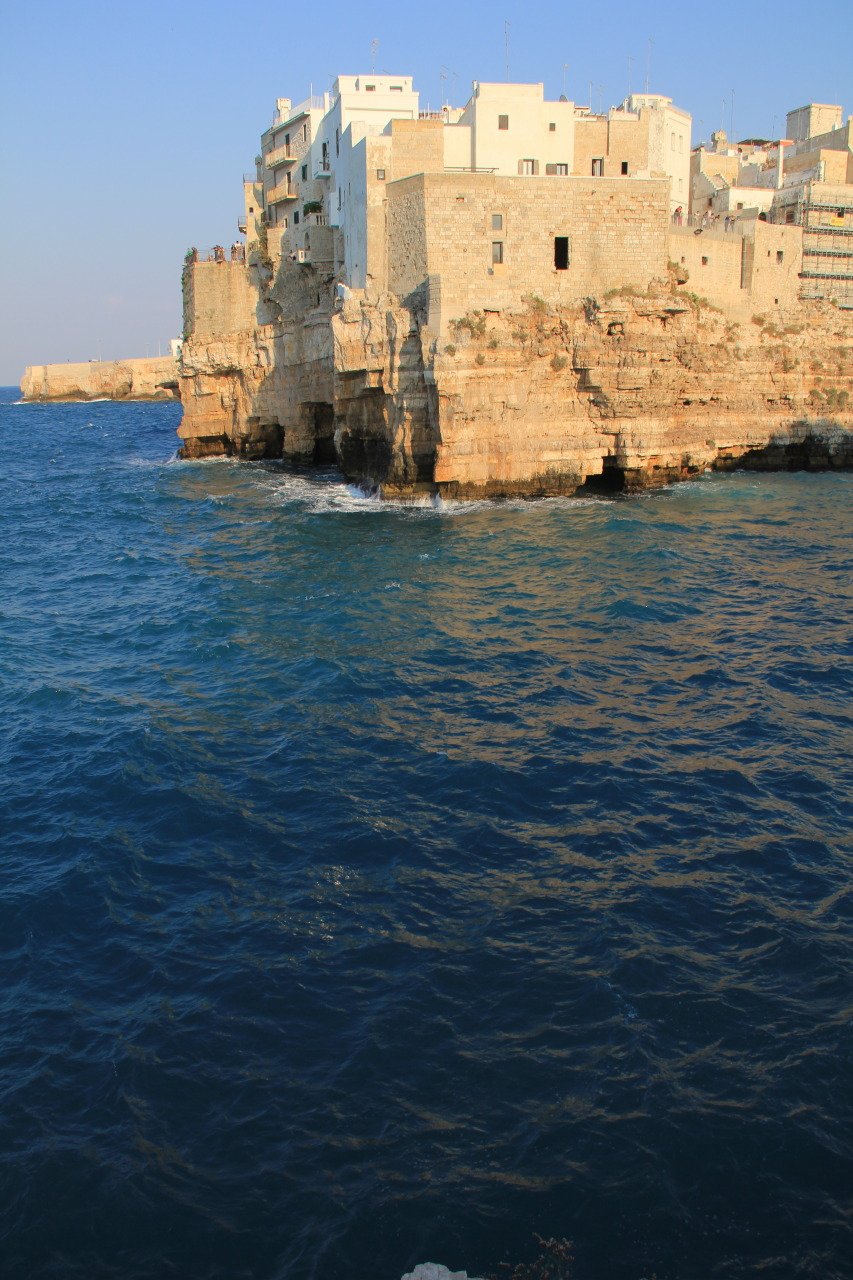
\includegraphics[width=0.4\textwidth, height=5cm, keepaspectratio]{../Bilder/Sommer2012/54.jpg}
    \caption{Polignano al Mare}
  \end{centering}
\end{wrapfigure} 

Kurz nach 13:00 Uhr machten wir uns auf den Weg mit Sack und Pack um Polignano einen Besuch abzustatten.
Der Reiseführer versprach einen Parkplatz im Norden der Stadt und nach einem kurzen Besuch an der Tankstelle befanden wir uns dort, jedoch der Parklpatz war nicht in Sicht.
Ein Feld bot sich jedoch als Lösung für das leidige Problem an.
Auf diesem waren auch schon mehrere Autos parkiert.
Beim Eingang mehrere langatmige Italienische Schilder.
Jack wurde platziert und die Stadt mit meinem Fotoapparat erobert.
Das eigentliche Ziel war ein Restaurant, welches wir am Abend besuchen wllten.
Dazwischen nutzten wir die Zeit für Sightsseing, Suche um wieder Pfus für den Bus zu bekommen und Apéros.
Mein Handy entschied sich nicht mehr zu funktionieren und eine kurze Rückfrage mit Nordeuroa ergab des Swisscom aussnahmsweise nicht Schuld daran sein sollte.
Viele Fotos später traffen wir kurz nach 20:00 Uhr zum Essen ein und bemerkten, dass uns der Campingplatz nur bis 22:30 zurück auf den Platz lassen würde.
Der Zweiakt-Cowboy würde uns sonst den Zutritt verweigern.
Ziemlich genau um 22:00 waren wir nach einem genialen Menü zurück beim Bus und machten uns sofort auf den Weg Richtung Monopoly.

Der Deputy erwartete uns schon an der Eingangspforte und wies mittels wilden Handzeichen daraufhin Ruhe zu bewahren.
Dass sollte er erstmals versuchen Jack beizubringen... Chantal verschwand direkt auf dem Stillen Örtchen.
Beim zurück räumen des Gepäcks wurde mir ziemlich schnell klar das gewisse Sachen fehlen.
Ein kurzer Blick auf das Schloss der Seitentüre bestätigte leider den Verdacht das Jemand den Schlüssel mit dem meist orangenen Griff und der Grösse 4 verwendet hat.
KAAACCKKKEEE.
Mein Rucksack, der Rucksack von Chantal, die Kameratasche von Chantal natürlich mit Inhalt, die neue Ledertasche und beide Necessaires hatten einen neuen unrechtsmässigen Besitzer gefunden.
Leider ein sehr unschöner Ausklang eines sonst schönen Tages.

\begin{figure}[H]
   \centering
      %\subfloat[CAPTION]{BILDERCODE}\qquad
   \subfloat{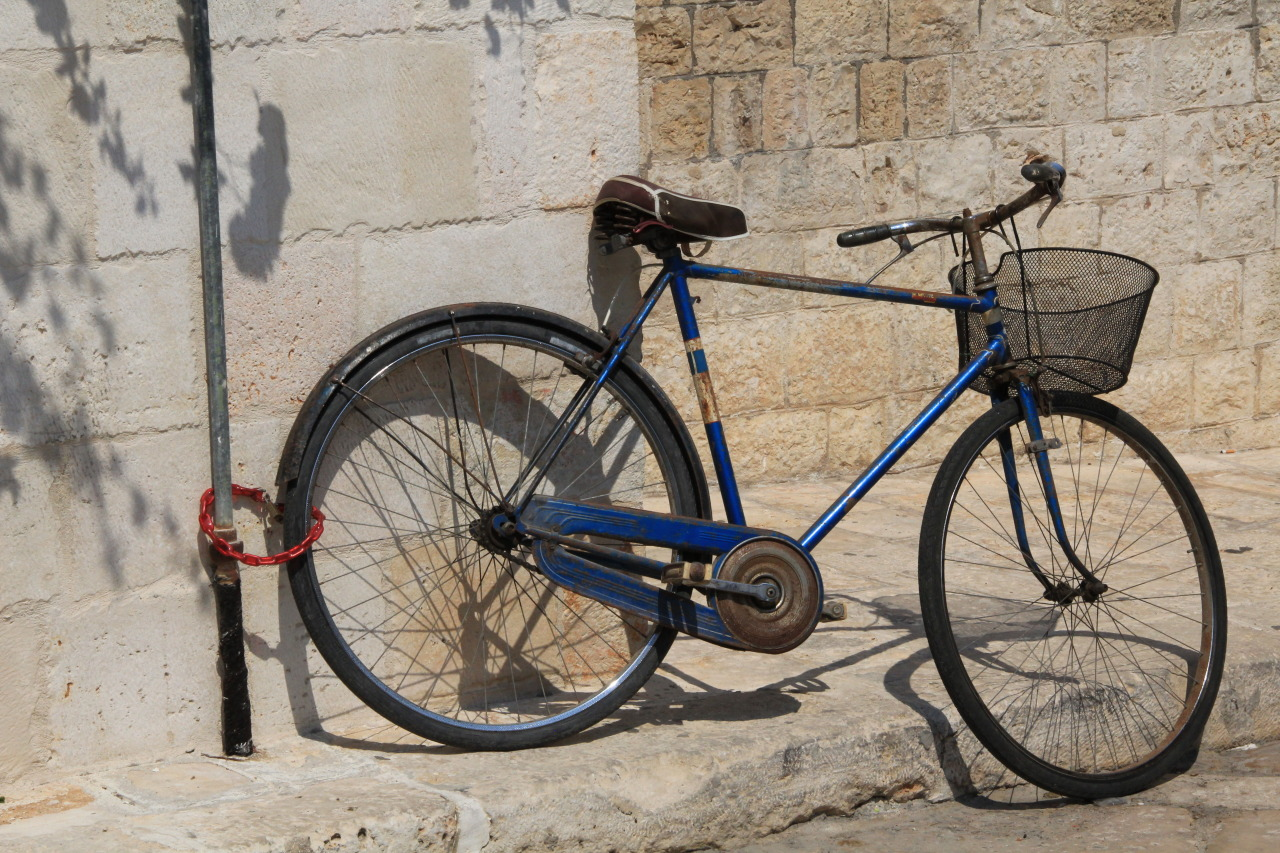
\includegraphics [width=0.3\textwidth]{../Bilder/Sommer2012/50.jpg}}\quad
   \subfloat{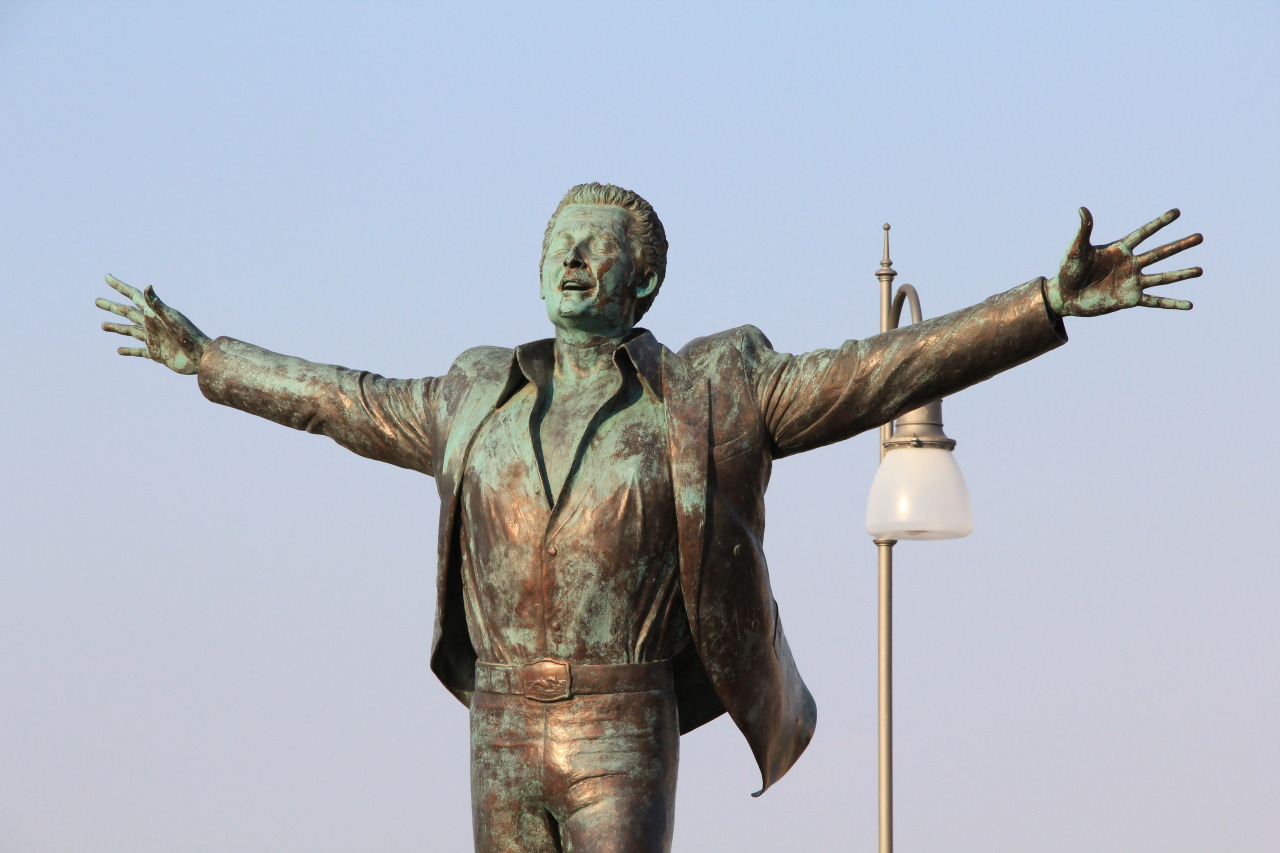
\includegraphics [width=0.3\textwidth]{../Bilder/Sommer2012/52.jpg}}\quad
   \subfloat{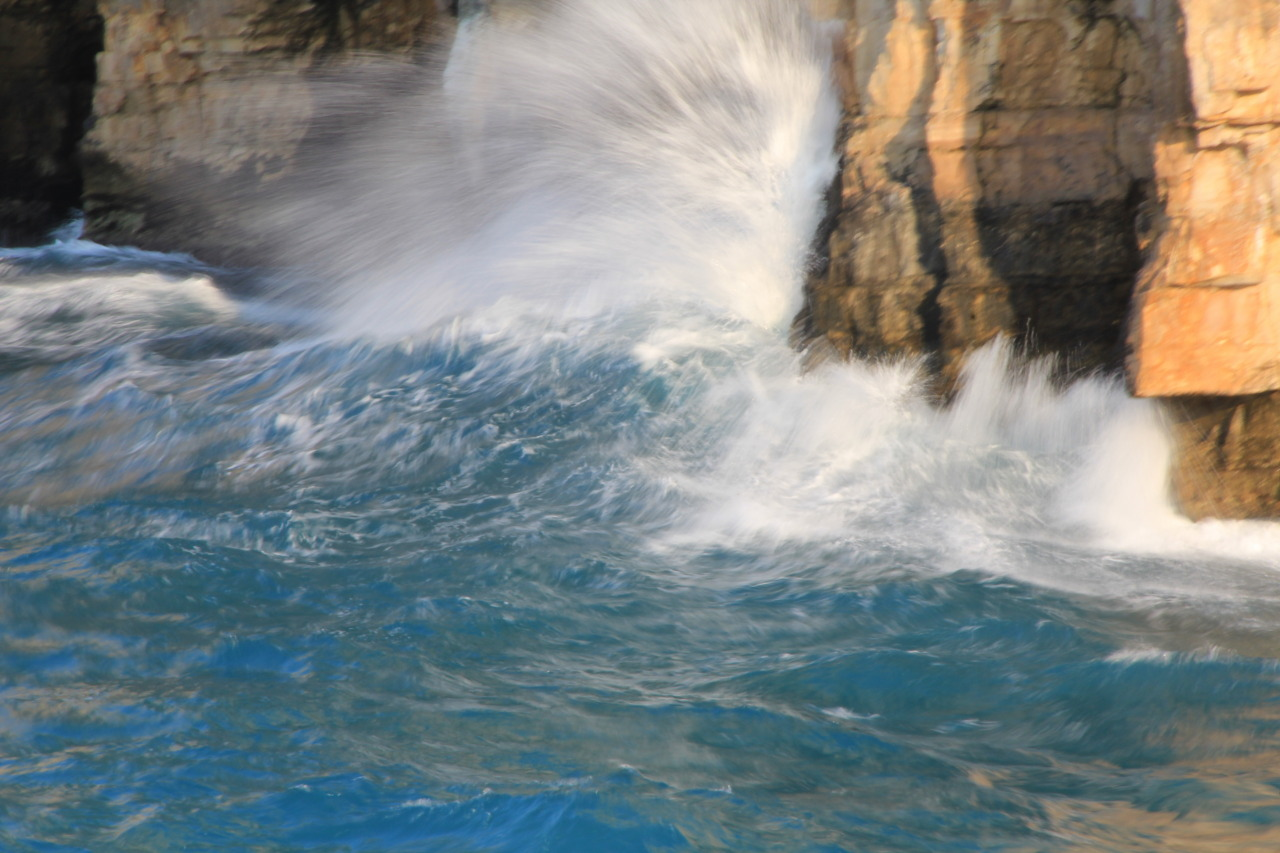
\includegraphics [width=0.3\textwidth]{../Bilder/Sommer2012/53.jpg}}\quad
   \caption[Polignano al Mare]{Polignano al Mare}
\end{figure}

\subsection{12.08.2012 Warten auf die Polizei}

\begin{wrapfigure}{L}{0.45\textwidth} 
  \begin{centering}
    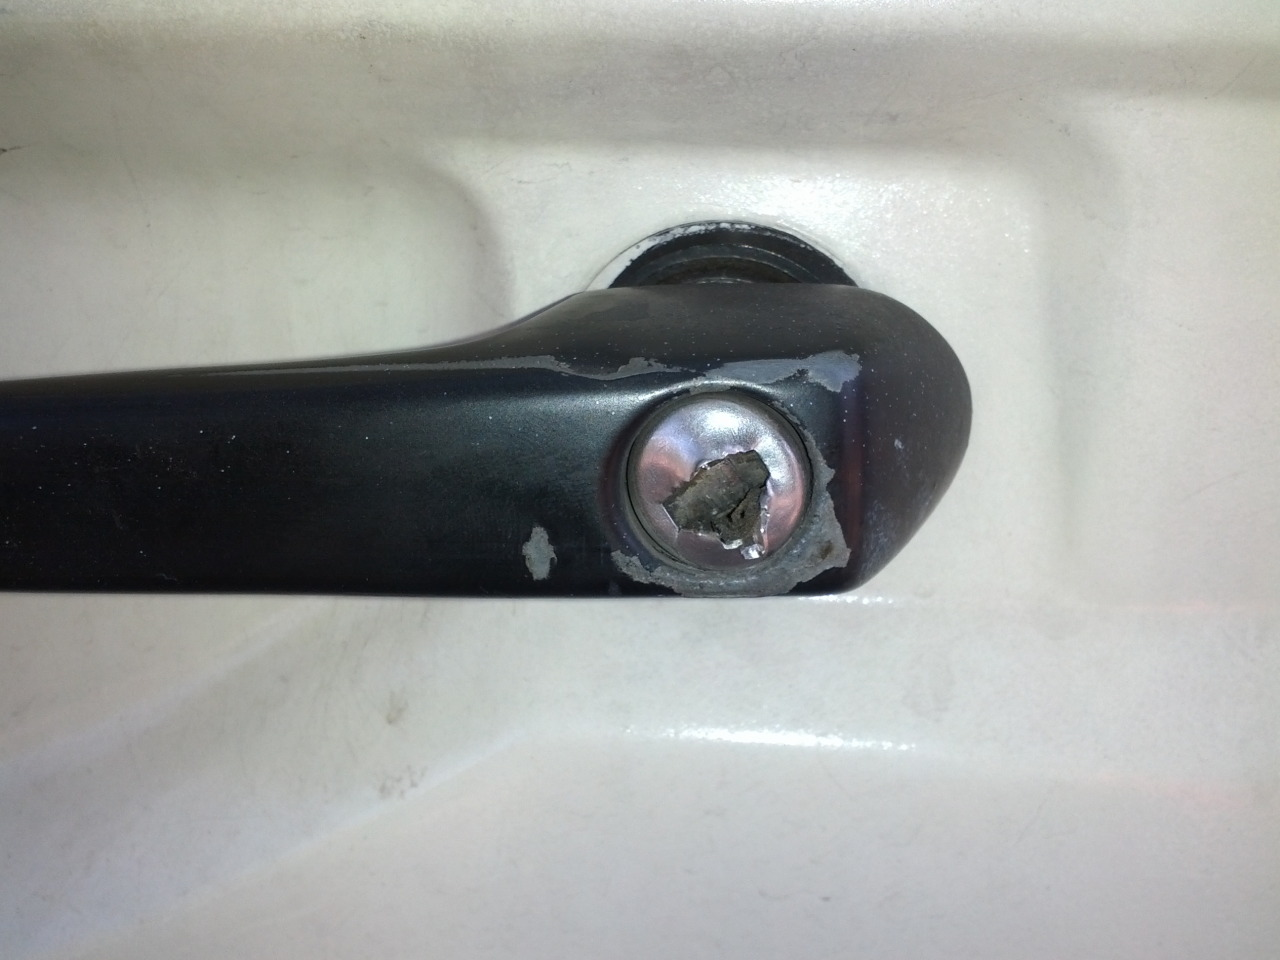
\includegraphics[width=0.4\textwidth, height=5cm, keepaspectratio]{../Bilder/Sommer2012/59.jpg}
    \caption{Ehemaliges Schloss}
  \end{centering}
\end{wrapfigure} 

Wir wollten den Diebstahl natürlich möglichst schnell der Polizei mitteilten und wenn möglich noch einmal einen kurzen Blick an den Tatort werfen.
Kurz vor 11 Uhr nach dem wir uns neue Zahnbürstchen und Zahnpaste organisiert hatten ginge es zurück nach Polignano.
Zuerst jedoch wurden wir von den Hütern des Campingplatzes, welche ihr kleines Reich verteidigen möchten, zurückgepfiffen.
Bei der Entsorgung des Abfalls hatten wir anscheinend einen Fehler begangen, der jedoch auch mittels Italienischen Fluchtiraden nicht behoben werden konnte.
Die Suche beim Parkplatz ergab leider kein nennenswertes Resultat.
Der \glqq Parkplatz\grqq war auch heute wieder gut besucht, trotzdem wollten wir uns möglichst schnell aus dem Staub machen, da auch der Ersatzschlüssel von Chantal im geklauten Gepäck war.
Dank der Suche nach dem Adapter für die Stromversorgung wussten wir schon wo sich das Polizeirevier befand und steuerten nach dem mehrmals kontrollierten Abschließen des Busses genau dieses an.
Der kahlköpfige Beamte wies uns sofort an das Touristenbüro aufzusuchen, da er nur italienisch sprach.
Die sich Mühe gebende Angestellte des Touri-Büros verwies und nach kurzer Rücksprache mit dem Polizisten eine Türe weiter an die Carabinieri
Nach 10 min Suchen fanden wir auch diese Gebäude und darin ein mit Orden behangener Ordnungshüter.
Wir hofften schon das die Hälfte der glitzernden Plaketten für ausserodentliche Englischkenntnisse verliehen wurde, wurden aber leider arg entäuscht, Der gute Mann versuchte sich geschickt mit Ausreden in die nahende Siesta zu flüchten und stellte sich dumm und taub.
Mit etwas Geduld fanden wir heraus, dass ein Kollege (des Englisch mächtig) um 16:00 Uhr an selber Stelle anwesend sein sollte.
Die Zeit dazwischen lagen wir am viel besuchten und noch mehr fotografierten Strand von Polignano und deckten uns mit den Artikel ein, die vom Saupack geklaut worden sind.

\begin{figure}[H]
   \centering
      %\subfloat[CAPTION]{BILDERCODE}\qquad
   \subfloat{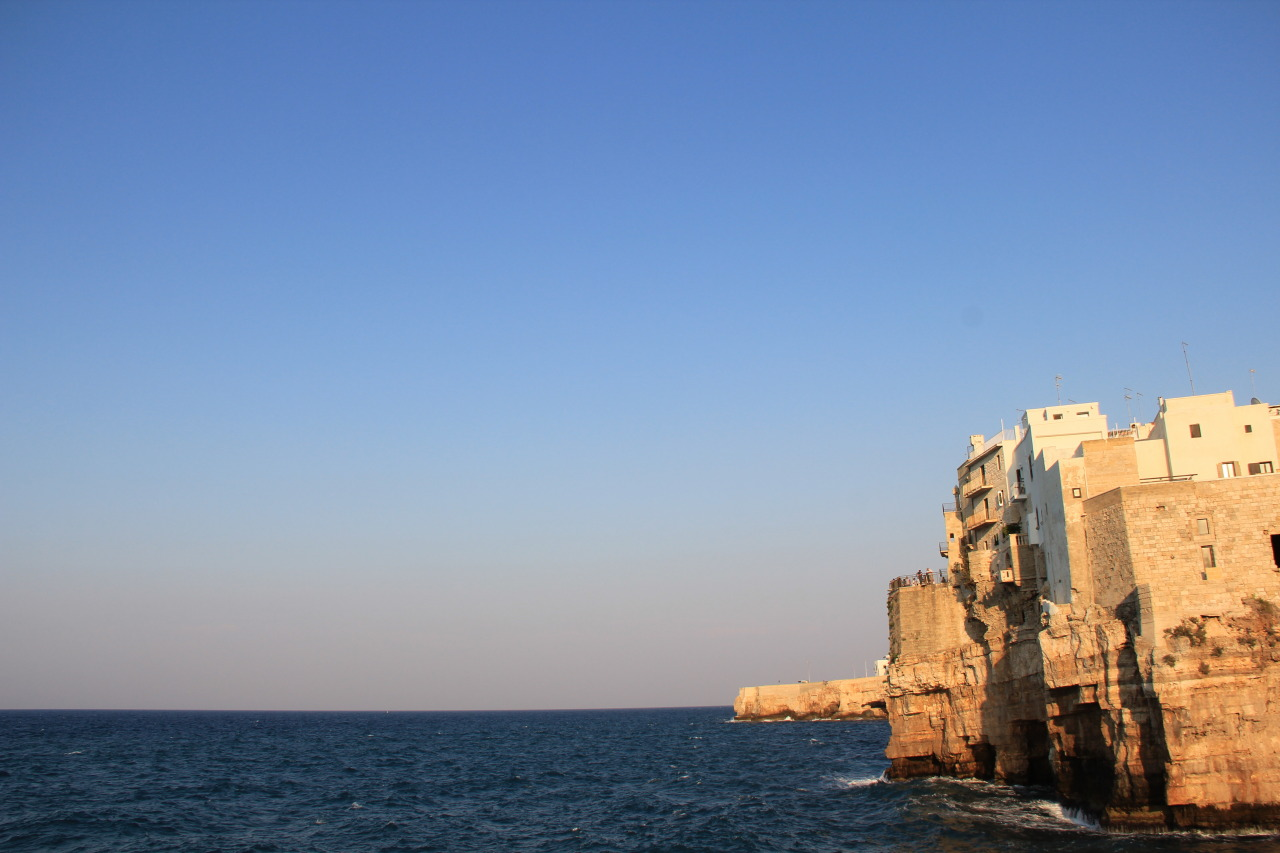
\includegraphics [width=0.3\textwidth]{../Bilder/Sommer2012/56.jpg}}\quad
   \subfloat{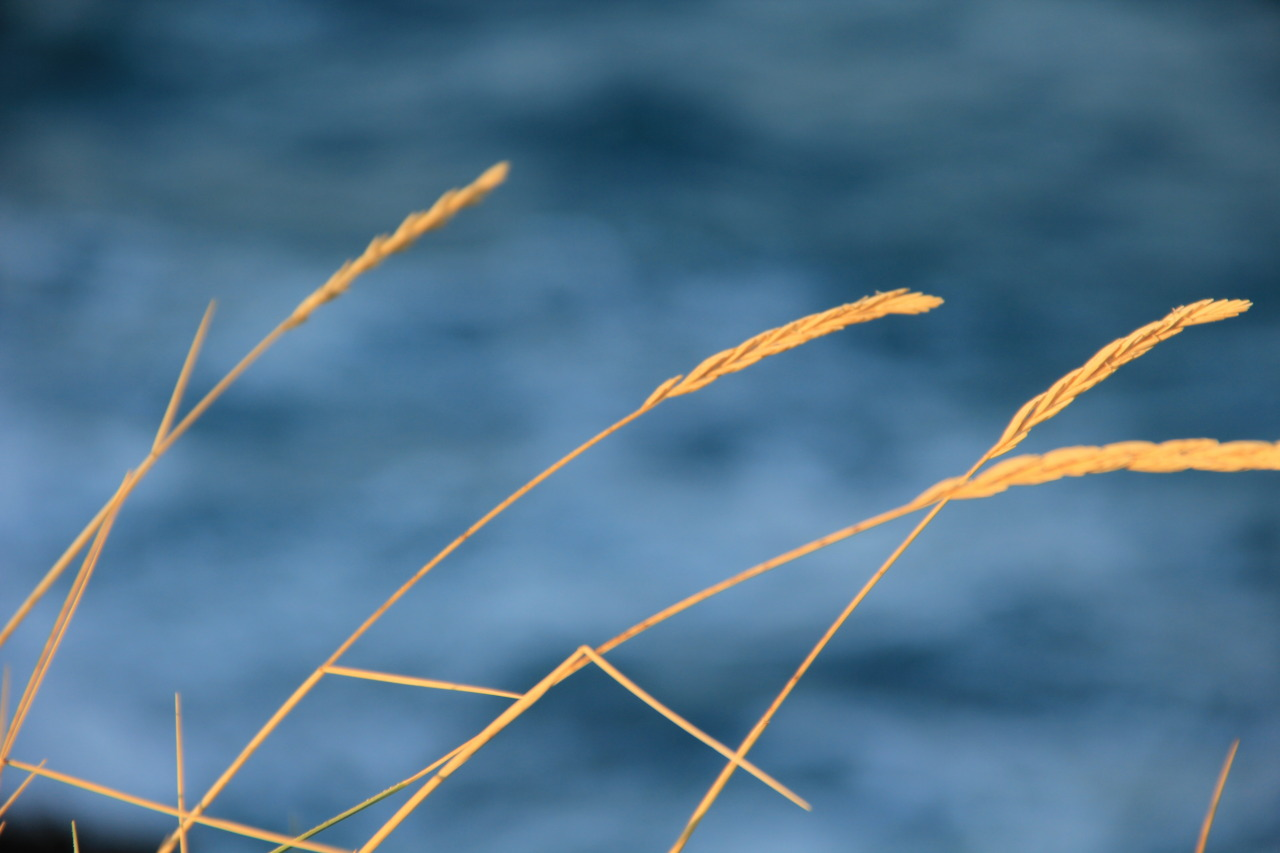
\includegraphics [width=0.3\textwidth]{../Bilder/Sommer2012/57.jpg}}\quad
   \subfloat{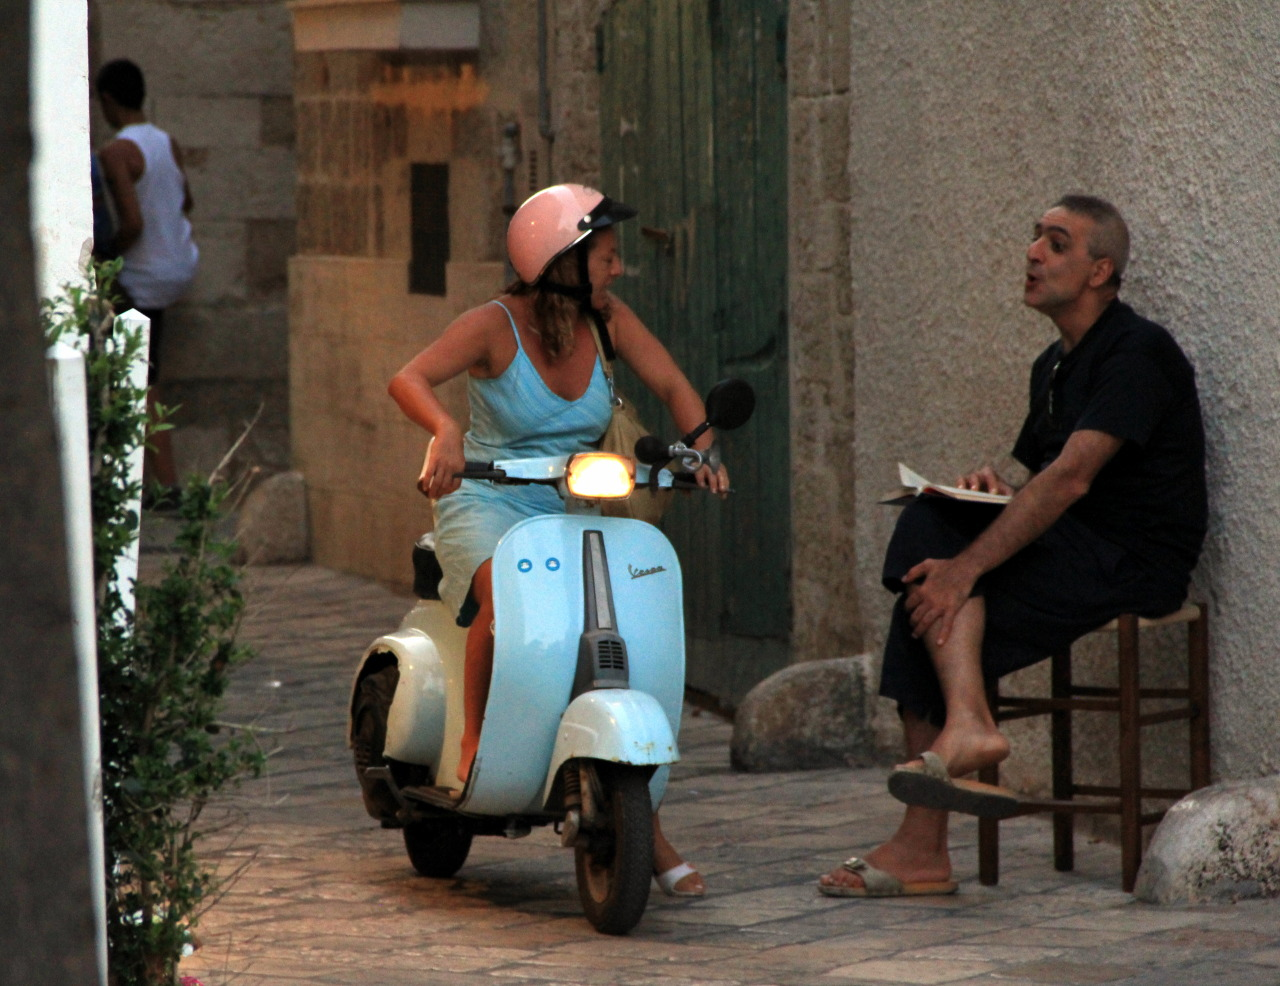
\includegraphics [width=0.3\textwidth]{../Bilder/Sommer2012/58.jpg}}\quad
   \caption[Polignano al Mare]{Polignano al Mare}
\end{figure}

Zurück auf dem Posten waren die anwesenden Polizisten zwar sehr Hilfsbereit, konnten jedoch in etwa so gut Englisch wie ich Französisch.
Vor allem das Diktieren der geklauten Gegenstände wurde zu einem Ratespiel \`a la Tabu, Montagsmaler oder \glqq Ich seh etwas was du nicht siehst \grqq.
Trotz allem verlief das Ganze relativ schnell und nach 3/4 Stunden waren wir auf dem Weg nach Monopoli.
Unsere Wasservorräte waren arg strapaziert worden und wir mussten noch Linsenmittel für Chantal sowie endlich ein Kabel für Jack finden.
Nach mehreren Eurospars, Lidl und anderen Supermercati hatten wir zwar alles erdenkliche gefunden, vom Linsenmittel fehlte aber noch jede Spur.
Gegen den Abend wurde es richtiggehend kühl.
Ja, unglaublich aber wahr, Chantal verkroch sich schon bald unter eine Decke und wir aßen unsere mittlerweile gut bekannten Pasta.
Der Besuch eines Bewohners des Campinglatzes der mehrere Jahre für Rolex in Genf gearbeitet hat und erkundigte sich wie man Ricola richtig ausspricht, sorgte für eine willkommene Aufheiterung.

\subsection{13.08.2012 Neue Woche neues Glück}

\begin{wrapfigure}{L}{0.45\textwidth} 
  \begin{centering}
    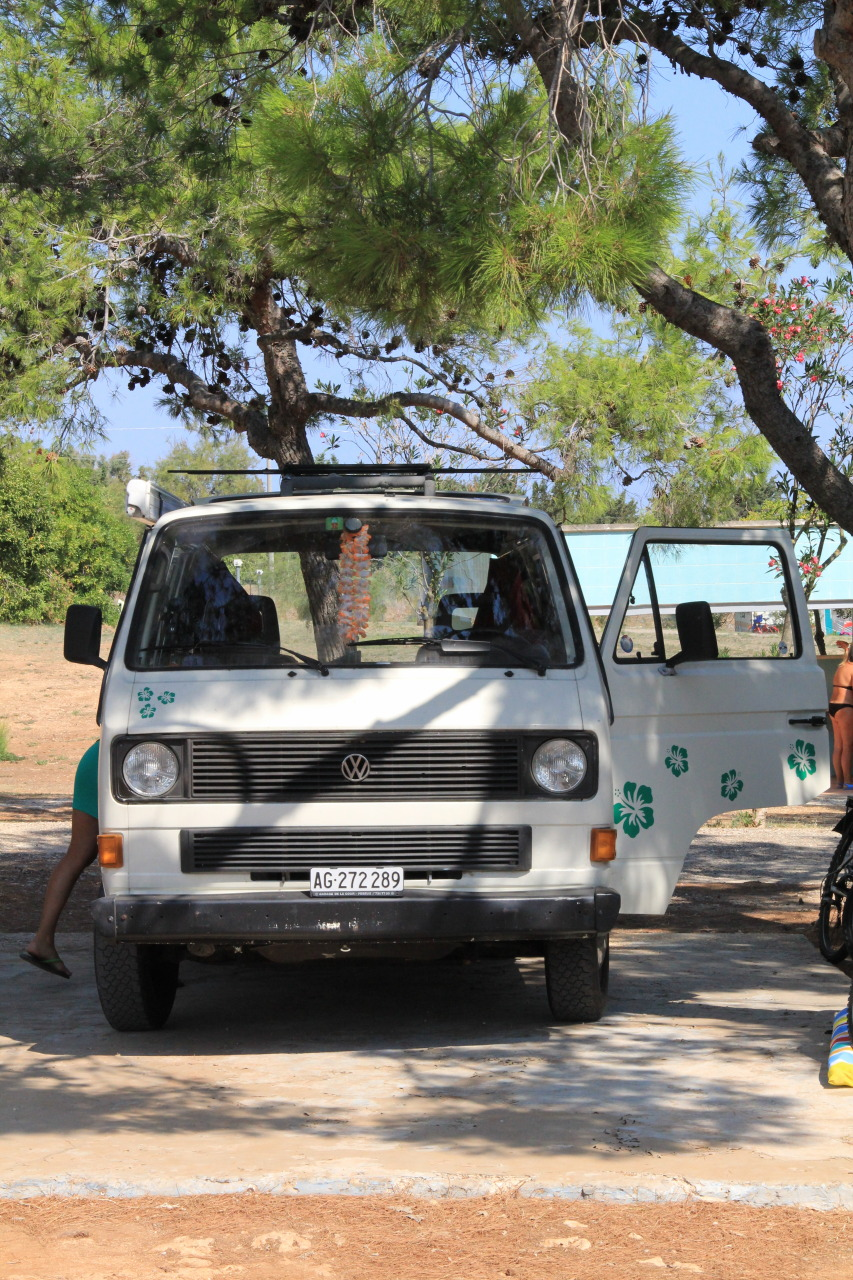
\includegraphics[width=0.4\textwidth, height=5cm, keepaspectratio]{../Bilder/Sommer2012/60.jpg}
    \caption{Campingplatz San Stefano}
  \end{centering}
\end{wrapfigure} 

Die neue Woche brachte zuerst einmal etwas Neues: Regen! Kurz nach dem aufstehen fielen fette Regentropfen vom Himmel.
Die Markise ausgefahren und wir konnten trotzdem gemütlich zmörgelen.
Wir nutzten die nasse Pracht gleich um die Scheiben von Jack zu reinigen.
Gut verteilt ist halb geputzt.
Durch das Wetter fiel der Strandtag buchstäblich ins Wasser.
Wir zogen uns noch einmal in den Bus zurück schauten Filme uns ich begann mit dem Studium des Kroatien-Reiseführers, welcher die Vorfreude beträchtlich steigerte.
Mitte Nachmittag besserte sich das Wetter und wir begaben uns per Bike nach Monopoli.
Am stadteigenen Strand hüpfte Chantal kurzerhand ins Wasser, während dem ich mich über die fehlenden Badehosen meinerseits ärgerte.
Beim Streifzug durch die Stadt um das langersehnte Linsenmittel zu finden trafen wir auf eine vorzügliche Gelaterie, welche man natürlich nicht einfach links liegen lassen konnte.
Schlussendich wurden wir dann endlich fündig und eine letzte Pendenz der Diebstahlliste konnte abgehackt werden.
Chantal hatte endlich ihr Linsenmittel.
Ein Grund zum Feiern! Wir ließen uns den Caipiroska und den Latino-Americano die Kehle herunter rollen und fanden schon bald darauf ein kleines Feines Restaurant das Chantal mit Fisch versorgen konnte.
Für mich wurde ein weiteres Mal die Spaghettipresse angeworfen und der Fischer mit der Suche nach Meeresfrüchten beauftragt.
Die wiederum dunkle Fahrt zurück zum Camping verlief dann reibungslos

\subsection{14.08.2012 Ohne Drucker keine Fahrt}

\begin{wrapfigure}{R}{0.45\textwidth} 
  \begin{centering}
    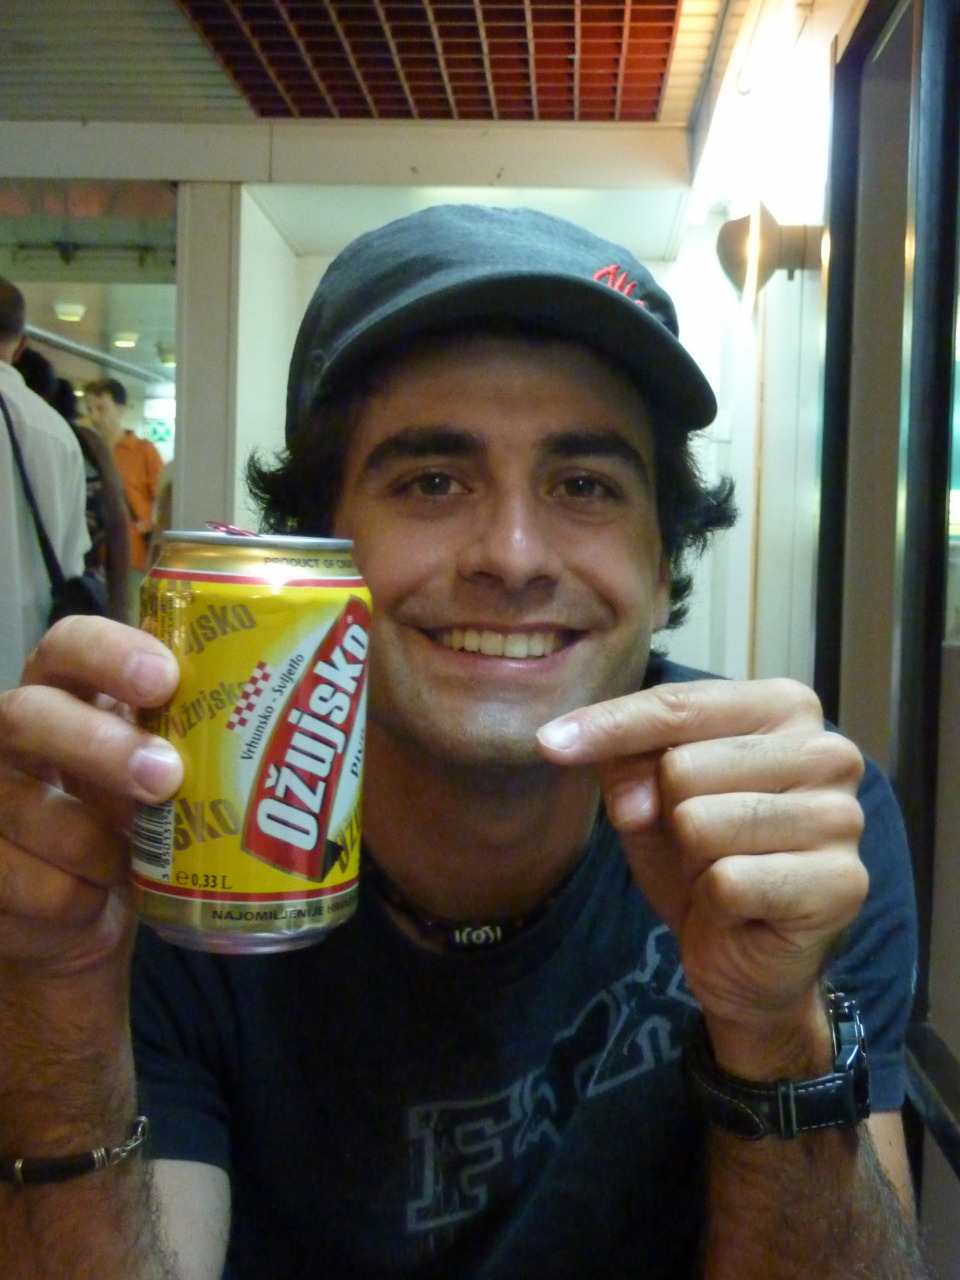
\includegraphics[width=0.4\textwidth, height=5cm, keepaspectratio]{../Bilder/Sommer2012/62.jpg}
    \caption{Erster kulturelle Kontakt mit Kroatien}
  \end{centering}
\end{wrapfigure} 

Auch heute wurden wir nicht wie gewohnt durch Sonnenstrahlen geweckt, sondern eher durch Wolken und kurze Schauer.
Die Fahrt nach Bari, die Stadt, welche laut Reiseführer ein Chaos sein soll, stand heute auf dem Fahrplan.
Freude herrscht.
Zuerst musste jedoch noch einmal das Födli ins Meer gehalten werden.
Nach dem Auschecken besuchten wir den nahegelegene Strand, welcher jedoch nicht gerade eine Augenweide war.
Scharfe Klippen verunmöglichten ein Liegen und um zum Wasser zu kommen waren Ninja-Kenntnisse von Not gewesen um den Rasiermesserscharfen Steinen auszuweichen.
Diese Umstände verhinderten nicht einen wahren Menschenstrom, welcher es sich irgendwie (wie auch immer) am Strand bequem machte.
Wir zogen weiter gen Norden und fanden beim zweiten Anlauf einen herrlichen Sandstrand mit Bistro.

Beim durchstöbern eines zweiten Reiseführers blieben uns glatt die bestellten Orechiette im Hals stecken.
Laut Aussage des Autors, war das Einreisen nach Kroatien nur mit Pass, nicht mit ID möglich.
So soll es jedenfalls für Schweizer sein.
Es stellte sich heraus, dass dieser Reiseführer um einiges aktueller war als der andere.
Hoppla.
Ich hatte meinen Pass zu Hause gelassen, da es laut TCS nicht nötig sei diesen mitzunehmen und den Pass von Chantal hatte Giovanni und seine Crew nun irgendwo in Palermo.
Das einzige was uns übrig blieb war zu hoffen das sich der sich als äusserst kompetent ausgebende Autor täuscht.

Die Fahrt nach und durch Bari verlief völlig Problemlos.
Der Hafen war gefunden, jedoch war das Büro bis 18:30 geschlossen.
Und ohne den Zettel war die Zufahrt zum Hafen nicht erlaubt und wurde durch grimmig Beamte der Guardia di Finanza kontrolliert.
Die einem Labyrinth ähnelnden Altstadt war schnell durchquert und ein Shoppingparadies eröffnete sich vor Chantals Füssen, welches sogleich erkundet werden wollte.
Ich ging auf die Suche nach einem WLAN um die unklare Situation betreffend Einreise zu klären.
Es zeigte sich, dass der TCS wirklich nichts von einem Pass erwähnt.
Also dürfte soweit alles in Ordnung sein.
Bosnien-Herzegowina verlangt jedoch einen Pass.
Diese müssen wir durchqueren, wenn wir Kroatien auf dem Landweg nach Norden durchfahren wollen.
Fähren bieten hier jedoch eine Alternative.

Kurz vor sieben fanden wir eine betrechtliche Schlange vor dem Schalter.
Auch eine Stunde später war die Schlange vor uns noch unverändert.
Nach hinten zeigte sie jedoch einen klaren Aufwärtstrend, was die Wartezeit betraf.
Ich klingte mich aus der Warteschlange aus um etwas essbares zu besorgen und den Wasserhaushalt wieder in Balance zu bringen und auch nach dem zurückkommen mit Hot Dog das gleiche Bild.
Jetzt jedoch waren schon etliche Personen damit beschäftigt den Drucker für die Tickets zum laufen zu bringen.
Leider noch ohne Erfolg.
Uns beschäftigte noch eine weitere Frage: Warum standen alle Wartenden mit Gepäck in der Schlange? Auch nach mehrmaligen Erkundigen konnte uns keiner eine Antwort daraufgeben ob wir am richtigen Ort anstehen.
Hinter uns stand ein Pärchen aus Bosnien an, mit denen wir schnell ins Gespräch kamen.
Beide sprachen relativ gut Englisch und erzählten uns etwas über Kroatien, Bosnien, Ihre Reise nach Italien (14 Stunden Shoppingtrip, crazy) und die Politische Lage in ihrem Land.
Während dem spannenden Gespräch konnte der Drucker überzeugt werden Tickets auszuspucken und kurz nach 20:00 waren wir an der Reihe und natürlich wurde der Fahrzeugausweis verlangt, welcher sich auf dem Parkplatz im Bus befand.
Los gerannt und diesen geholt und wild fluchend mit allerlei Zettel versehen mit Barcodes versuchten wir den Hafen zu entern.
Vergebens.
Das Schiff stand zwar in Sichtweite, jedoch wurden wir zu einem 3 km entfernten anderen Tor geschickt.
3 km Richtung Westen um Nachher wieder 3 km nach Osten zu fahren um an der anderen Seite der Barriere (vor welcher wir gerade standen) aufzutauchen.
Anstehen für Zoll und andere Jacks, eh Checks.
Am Viertel ab 9 hatten auch wir es geschafft und der Bus war im Bauch der kleinen Fähre verstaut.
Die Kabine war dann schnell gefunden und mit einer Stunde Verspätung ging die Fahrt nach Kroatien los.
Das erste Kroatische Bier wurde genossen, zu Essen gab es nichts mehr. Kurz darauf dösten wir ein...

\subsection{15.08.2012 Dubvronic}
Um 5:30 klingelte der Wecker, Frühstück gab es von 6-7.
Das Schiff holte die stündige Verspätung problemlos auf und schon während dem zerkleinern des Toasts kam die \glqq Skyline \grqq von Dubrovnic in Sichtweite.
Nach dem anlegen meinte ein Kroatischer Zollbeamte, dass uns der Kleber mit dem berühmten \glqq CH \grqq fehle.
Da wie jedoch Schweizer seien vertraue er darauf, dass wir einen solchen noch beschaffen werden.
Bei Italienern sei das eine ganz andere Geschichte.
Fügte er noch lachend hinzu.

\begin{figure}[H]
    \centering
    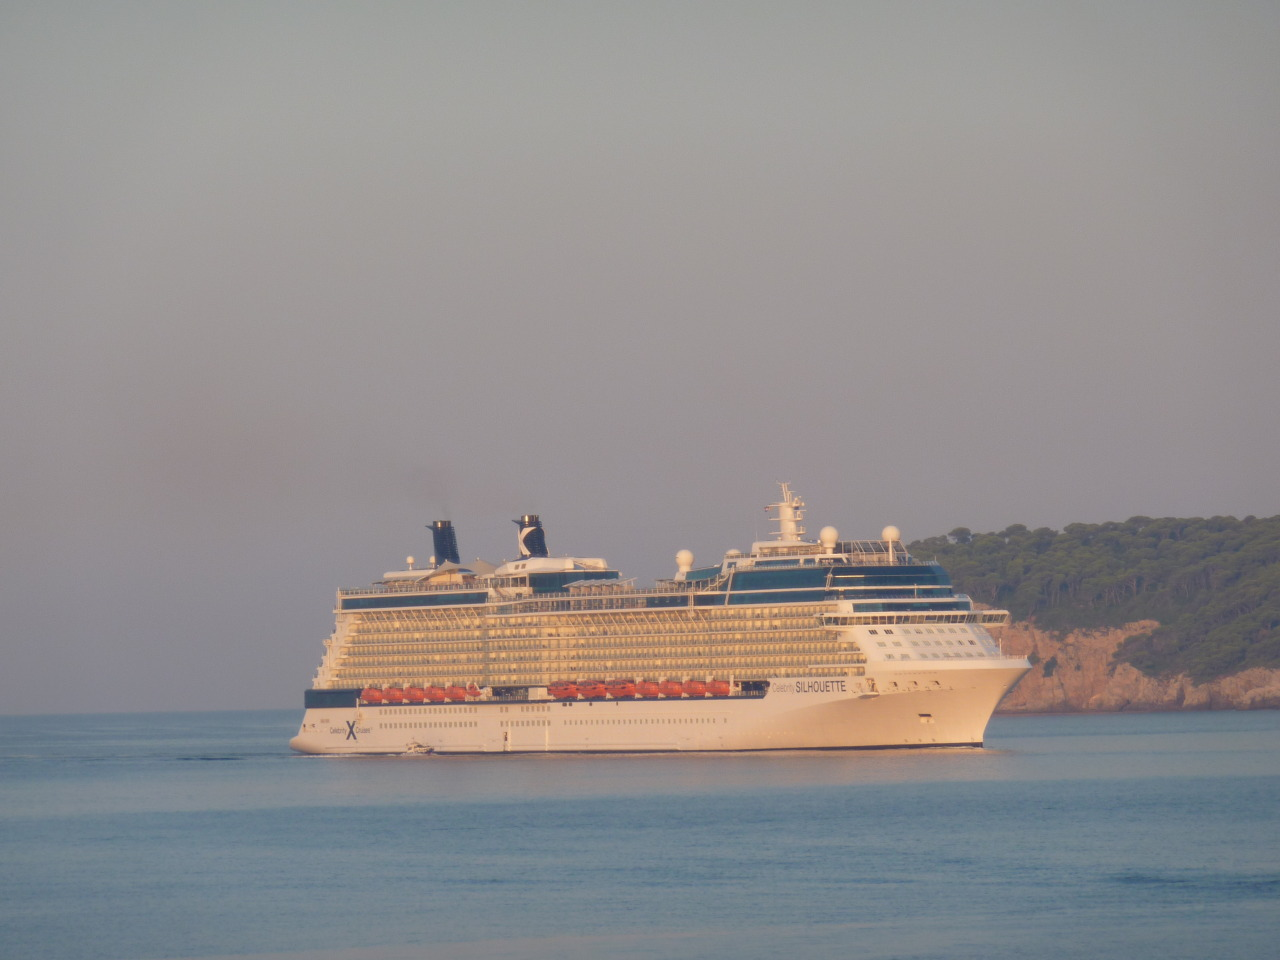
\includegraphics[width=0.5\textwidth]{../Bilder/Sommer2012/63.jpg}
    \caption{Schiff vor dem Hafen von Dubrovnic}
    \label{img:Sommer6}
\end{figure}


Der Camping Solitude war schnell gefunden und die nette multilinguale Empfangsdame versprach uns einen Platz, der jedoch erst ab 10:00 zur Verfügung stand.
Wir verbrachten die Zeit dösend auf dem Parkplatz.

\begin{wrapfigure}{R}{0.45\textwidth} 
  \begin{centering}
    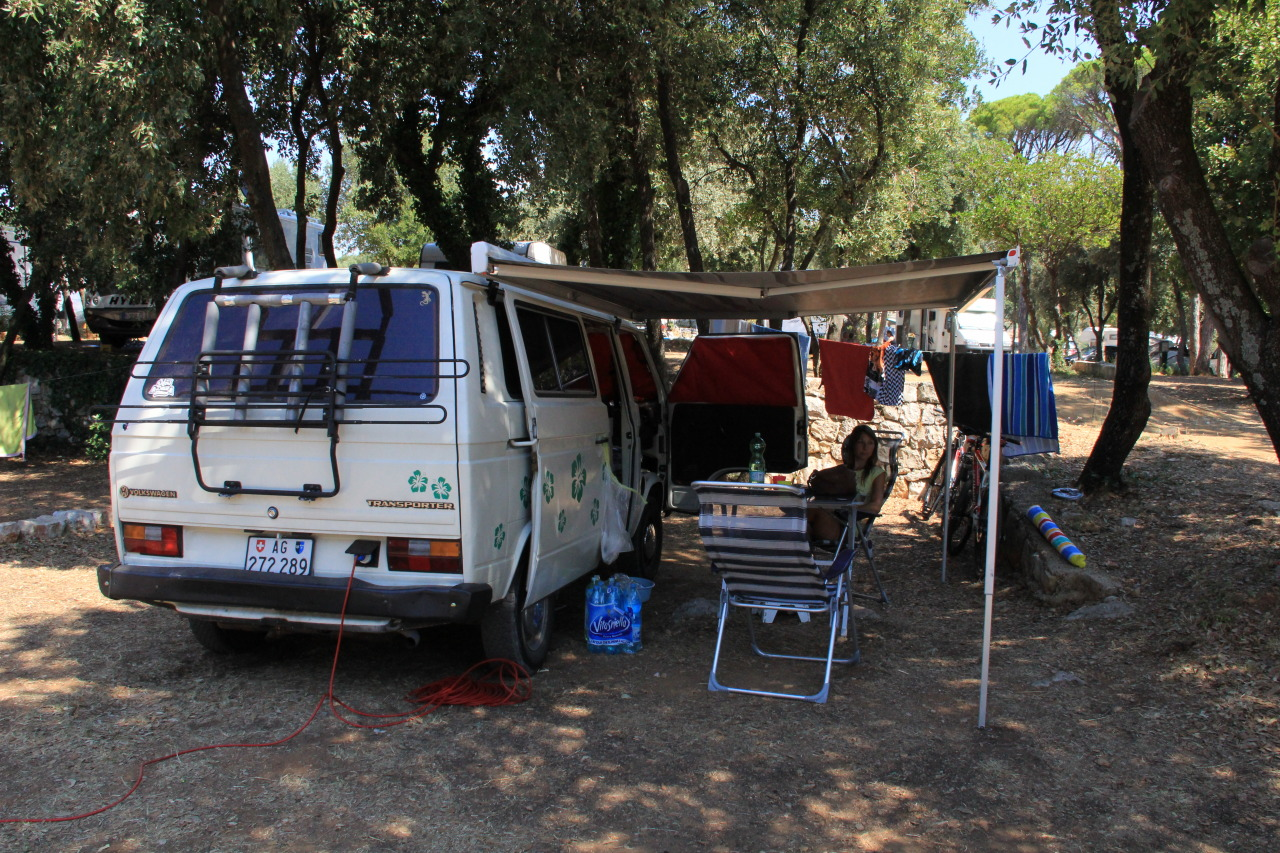
\includegraphics[width=0.4\textwidth, height=5cm, keepaspectratio]{../Bilder/Sommer2012/64.jpg}
    \caption{Camping Solitude}
  \end{centering}
\end{wrapfigure} 

Nach dem Beziehen des Platzes, stand auch schon die erste Velotour auf dem Programm.
Richtung Altstadt sollte es gehen.
Nach einer halben Stunde erreichten wir diese durchgeschwitzt.
Wir waren natürlich ein weiteres Mal in der grössten Hitze aufgebrochen.
Die Altstadt von Dubrovnic war an den Menschenmassen zu erkennen.
Man könnte meinen es sei Stadtfest.
Wir flüchteten schnell in die Seitengassen und an den wunderschönen Hafen, um die Beine ins Meer zu halten, welches Glasklar die Hafenmauern umspülte.
Nach einer halben Stunde wurde ich schon das erste Mal ein Opfer von einer fiesen Krebs-Attacke.
Diese kleinen Biester kletterten die Senkrechte Mauer mühelos empor.
Nach einem kurzen Abstecher im Nike Store ( Wie war der Umrechnungsfaktor Kuna-CHF?) ging es hinauf auf den Hügel neben der Stadt um die wunderschöne Aussicht zu geniessen.
Eine Gondelbahn bringt einem mühelos hinauf und die Sicht ist atemberaubend.
Wir entschlossen heute selber zu kochen und deckten uns nach der Rückfahrt im Campingeigenen Laden mit Wienerli und Thunfisch und Salat ein.
Die Wienerli waren nicht gerade der Renner der Rest verschwand jedoch äusserst schnell in unseren Magen.
Chantal bewiess ihr Können an der Waschmaschine und stockte unsere Kleidervorräte wieder auf. Zeit zum Schlafen...

\begin{figure}[H]
   \centering
      %\subfloat[CAPTION]{BILDERCODE}\qquad
   \subfloat{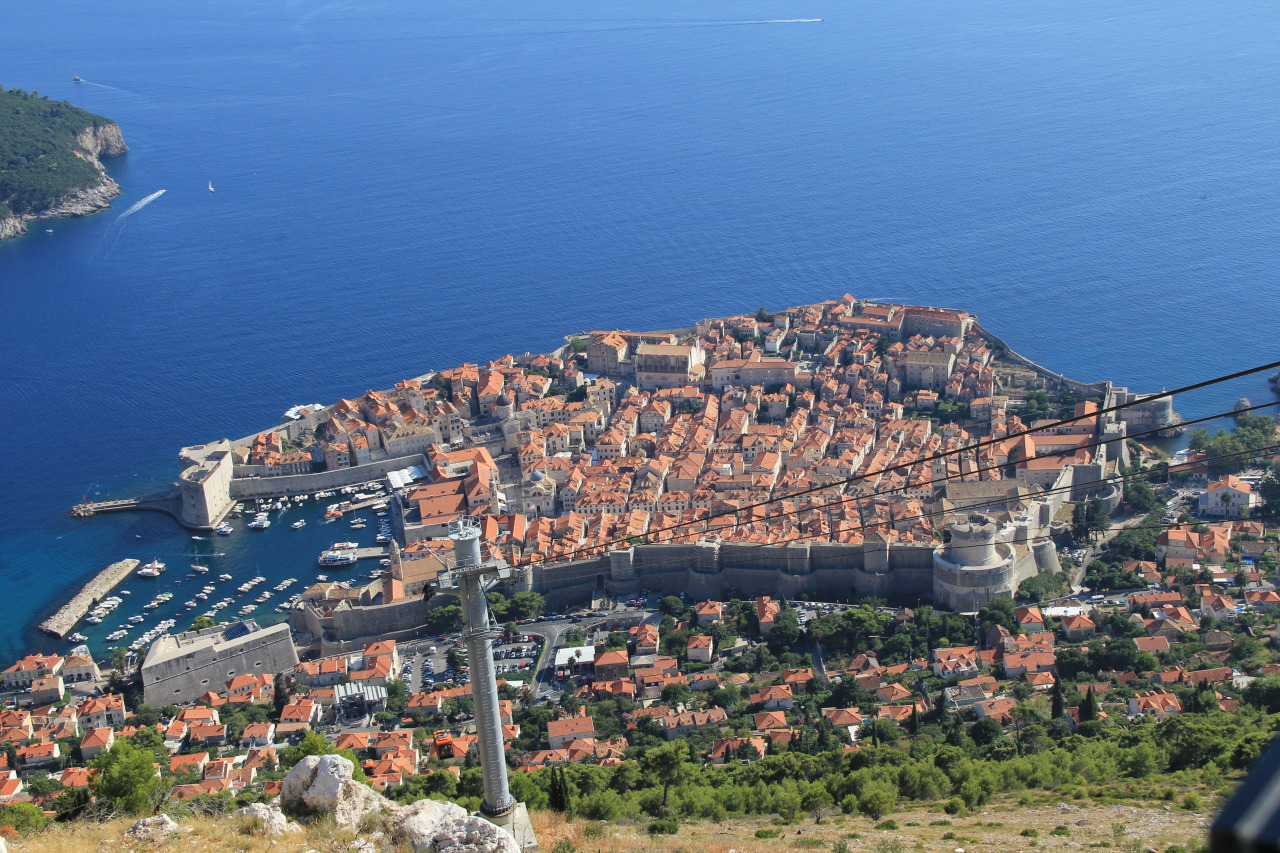
\includegraphics [width=0.3\textwidth]{../Bilder/Sommer2012/65.jpg}}\quad
   \subfloat{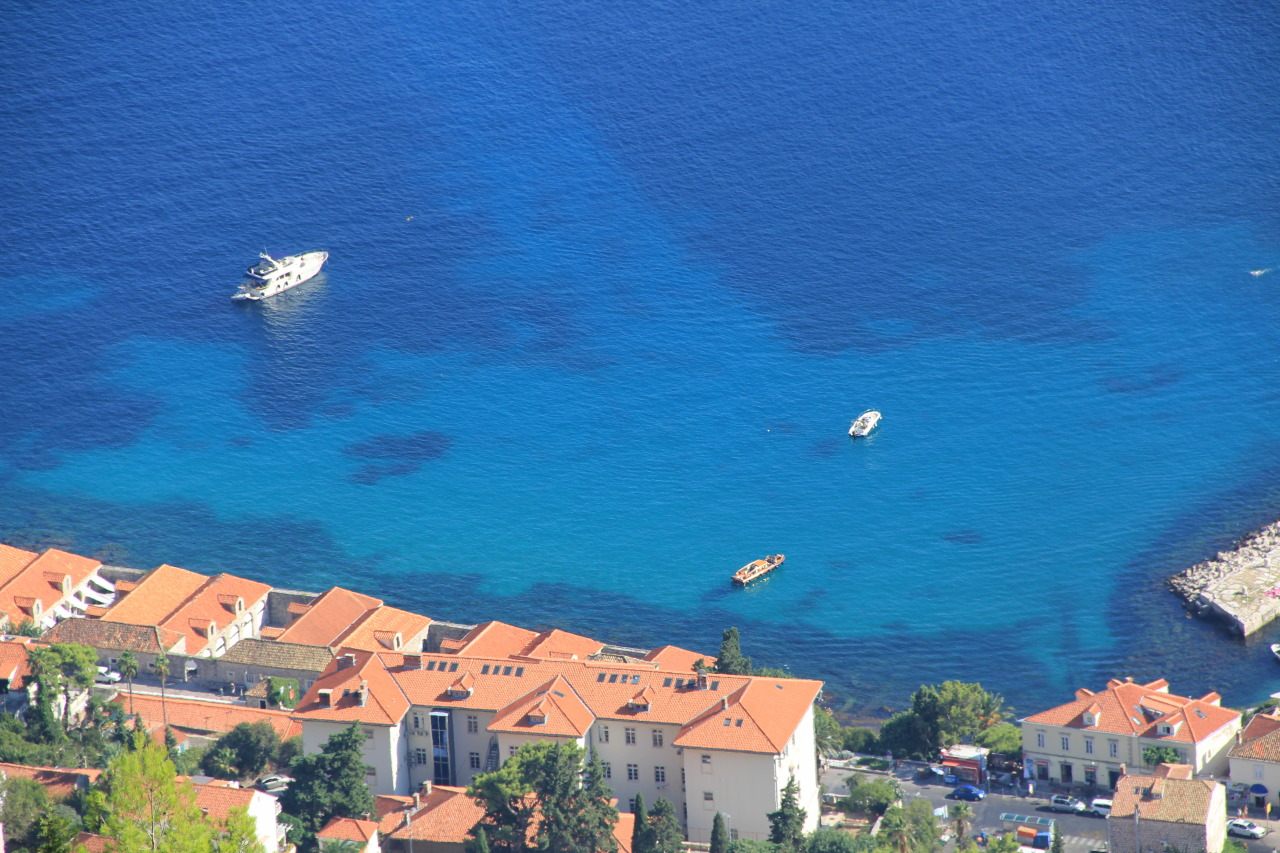
\includegraphics [width=0.3\textwidth]{../Bilder/Sommer2012/66.jpg}}\quad
   \subfloat{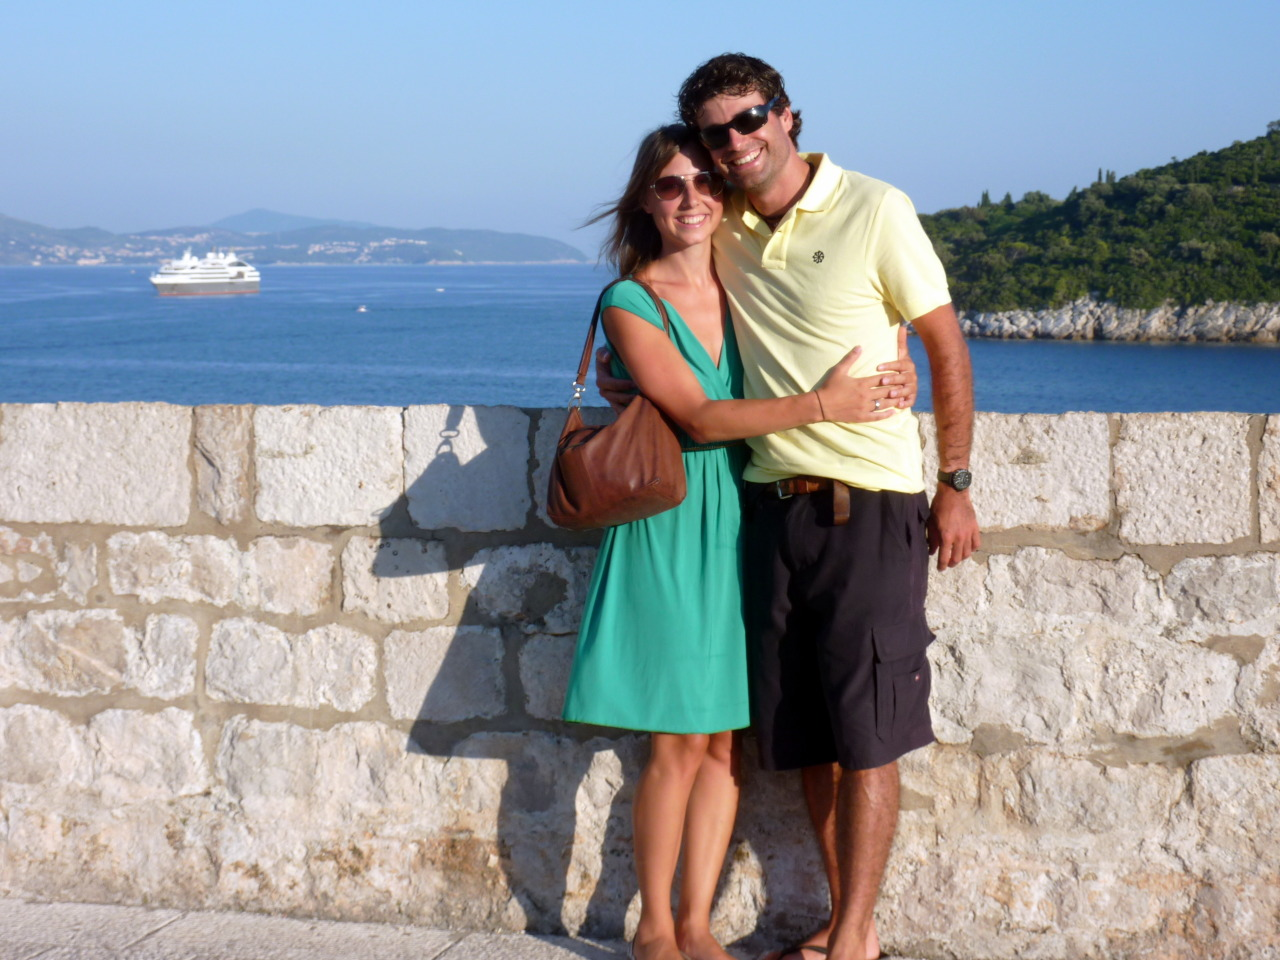
\includegraphics [width=0.3\textwidth]{../Bilder/Sommer2012/68.jpg}}\quad
   \caption[Dubrovnic]{Dubrovnic}
\end{figure}

\subsection{16.08.2012 Erste Schnorchelversuche und Mauerwanderung}
Nach dem anstrengenden sportlichen Tag gestern war heute wiedermal ein Strandtag angesagt.
Die nahrhaften Gipfeli und die riiiesige Wassermelone zum Zmorgen waren ein guter Start in den Tag.
Schön ausgeschlafen und gestärkt machten wir uns auf den Weg zum Campingstrand.
Dieser war ziemlich überfüllt aber sehr schön: glasklares Wasser und eine schöne Aussicht auf Inseln, die schöne Brücke vor Dubrovnik und die Gebirgszüge.
Wir verbrachten den Nachmittag mit Faulenzen und Baden.
Wir versuchten uns auch im Schnorcheln (bei einigen sah man nur noch viiele Haare und der Schnorchel oberhalb vom Wasser ;)), doch ausser einigen Albinofischen sahen wir nicht viel spannendes (kein riesen Tintenfisch wie in Koriska :)).

Um 4 Uhr gings zurück zum Camping und dann mit den Velos nach Dubrovnik.
Diesmal war es etwas angenehmer und nicht mehr so erdrückend heiss wie gestern.
Dort angekommen, war unsere Mission: der Spaziergang über die berühmte Stadtmauer.
Touristen hatte es immer noch zu genüge und wir mussten nur schon für die Tickets um auf die Stadtmauer zukommen, anstehen.
Aber es ging ruchzuckzackzack und es lohnte sich wirklich.
Die Aussicht von der Stadtmauer auf die Altstadt und vor allem auf das Meer und
die vorgelagerten Inselchen war traumhaft.
Es ging 2 Kilometer (ungefähr eine Stunde) stegeli ufe und stegeli abe, was abenteuerlich und anstrengend war.
In jedem Gässchen und auf Dachterrassen entdeckten wir viele herzige Restaurants, von welchen ein feiner Duft zu uns wehte, was ziemlich gemein war, da wir richtigen Kohldampf hatten.
Daher sprinteten wir nach unserer Wanderung direkt in ein feines Restaurant.
Es gab weisses Risotto mit Garnelen, Spaghetti mit Meeresfrüchten und Muscheln,
Tintenfische, Schrimps und Fisch ... hmmmm das war lecker!:) Nach dem Essen rugelten wir zurück zum Camping wo ich schnurstracks in einen Tiefschlaf fiel.
Stefan schrieb noch fleissig an unserem Tagebuch, bevor es dann auch hiess: dobra vecer.

\begin{figure}[H]
    \centering
    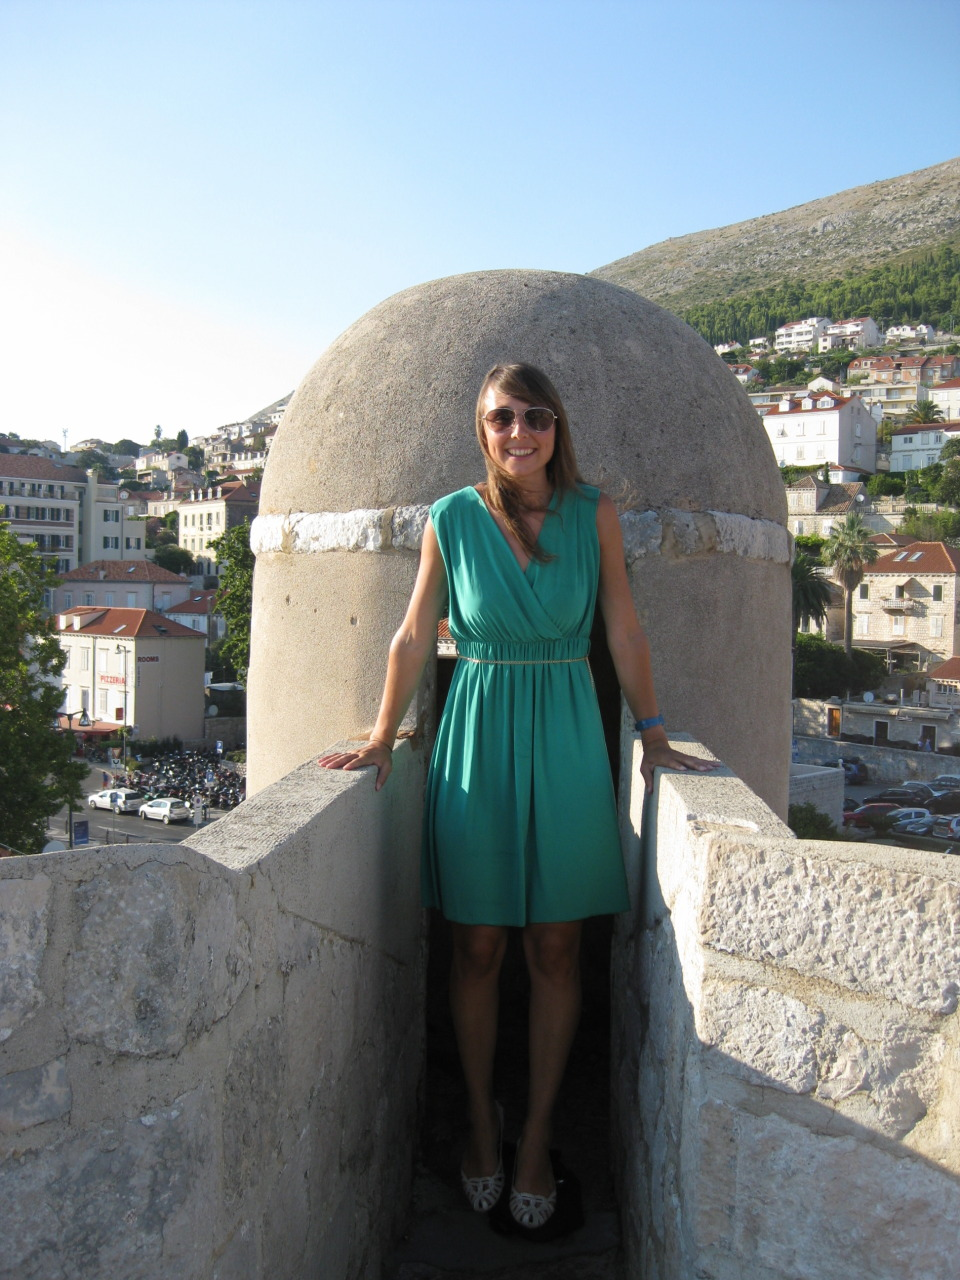
\includegraphics[width=0.3\textwidth]{../Bilder/Sommer2012/67.jpg}
    \caption{Auf den Stadtmauern von Dubvronic}
    \label{img:Sommer7}
\end{figure}

\subsection{17.08.2012 Korcula}

Heute war Aufbruchstimmung.
Die Insel Peljesac und die Insel Korcula stand auf unserem Programm.
All unsere sieben Sachen gepackt, machten wir uns auf den Weg und schon bald waren wir aus Dubrovnik heraus, über die wunderschöne Brücke vor Dubrovnik und auf der Küstenstrasse.
Diese verlief kurvenreich und mit einer atemberaubenden Aussicht auf das Meer und die zahreichen Inselchen.
Die Fahrt durch die Insel Peljesac war sehr gemütlich; viel Wald, einige Dörfer und ein paar Burgen mit ihren riesigen Festungsmauern.
Die Stadt Ston hat sogar die längste Festungsmauer (5km) von Europa.
Zuerst wollten wir auf einem kleinen abgelegenen Campingplatz in Trpanj übernachten, doch dann entschieden wir uns sogleich nach Orebic, welches am Ende der Insel liegt und Ausgangspunkt für die Insel Korcula ist, zu fahren.

\begin{figure}[H]
    \centering
    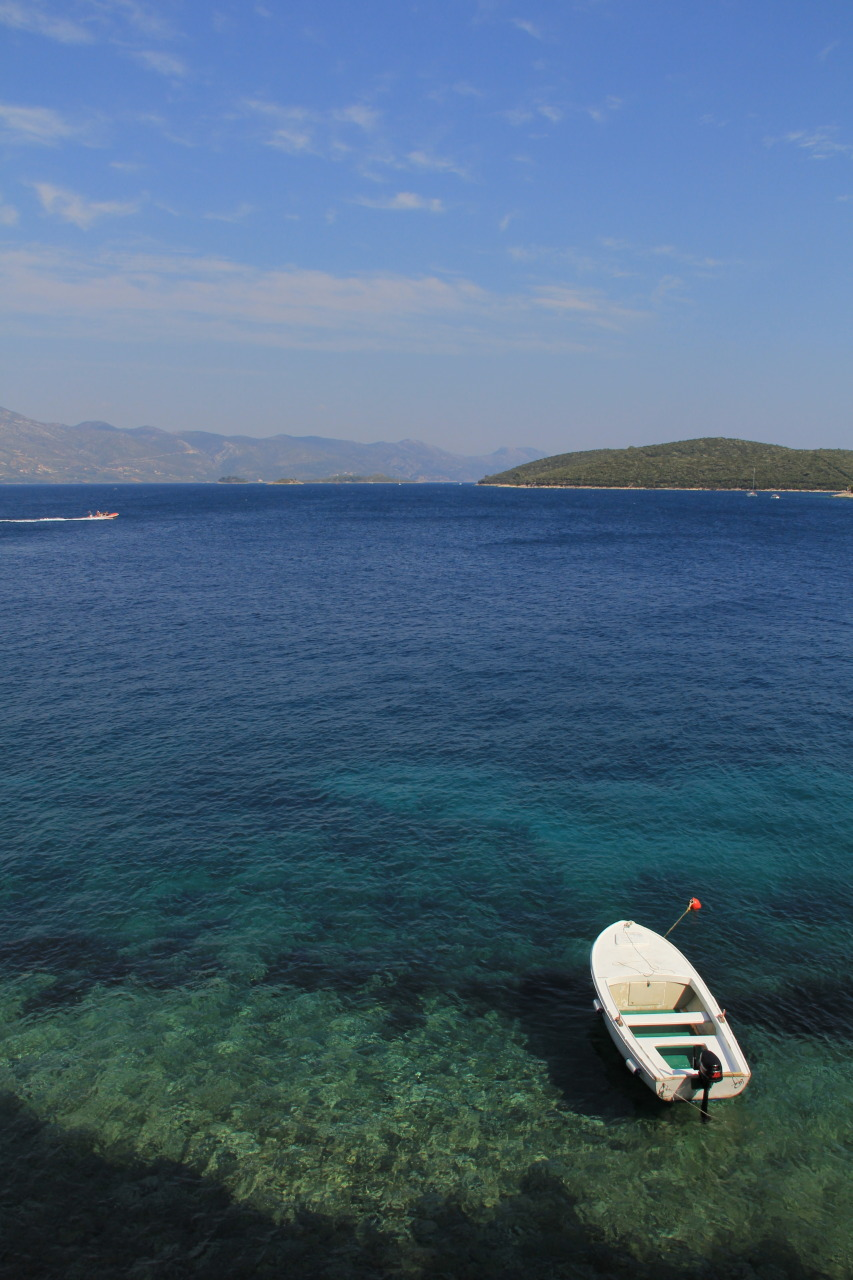
\includegraphics[width=0.3\textwidth]{../Bilder/Sommer2012/74.jpg}
    \caption{Korcula}
    \label{img:Sommer8}
\end{figure}

Wir hatten Glück und haben ohne langes Warten eine Fähre erwischt.
Jupii, das Insel-Hopping kann beginnen;) Schon nach ungefähr 20 Minuten waren wir in Korcula.
Ich habe im Reiseführer gelesen, dass Korcula auch sehr beliebt bei den Einheimischen ist, da das Klima sehr mild ist und die Winde Bora und Jugo nicht so stark sind (Die Bora kann sehr gefährlich sein, da es schon vorgekommen ist, dass Autos von der Küstenstrasse regelrecht weggewindet wurden).
Doch diese Information war irgendwie nicht so wahrheitsgetreu, denn schon auf der Fähre erblickten wir so viele Wind- und Kitesurfer wie noch nie, die ziemlich schnell herumflitzten und in Korcula angekommen, windete es uns fast davon.
Wir fuhren in die Stadt Korcula herein, schlenderten durch die Alstadt und gönnten uns eine Pizza in einem Restaurant direkt am Meer.
Dann machten wir uns auf nach einem nahegelegnen Camping, wo wir sofort einen Platz beziehen konnten.
Überraschung! Unser Nachbarauto war ein hellblauer VW-Bus aus Solothurn, welchen wir auf dem Camping in Dubrovnik schon gesehen hatten.
Und kaum ausgestiegen, kam deren Besitzerin schon auf uns zu und plauderte los über ihre Reservierungsmiseren und die beschwerliche Reise nach Dubrovnik.
Zudem zeigte sie uns die "schöne" Innenausstattung des VW-Buses (brauner Teppich).
Doch am besten gefielen mir die hellblauen Delphine, welche auf den Bus gesprayt waren ;) Sie gab uns noch ein paar gute Tipps wie z.B. das Insel-Hopping spart enorm Zeit.
Diese Aussage können wir nach einem weiteren Fährentripp, über welchen morgen berichtet wird, bereits widerlegen.
Nach diesen vielen Informationen gingen wir kurz an den Strand.
Doch wir hatten fast ein bisschen kalt, da es so windete wie noch nie..auf dem windstillen Korcula.
Zum Znacht gab es Suppe, Chips und ein etwas speziellen Wein aus der Region (in einer Cola-Flasche;)).

\subsection{18.08.2012 Wie kommen wir von dieser Insel weg?}
Der befürchtete Hang-over vom Inhalt der frisch erworbenen Cola-Flasche blieb zum Glück aus.
Wir standen schon um 8:00 auf um die Fähre nach (wir wissen leider nicht mehr wohin wir ursprünglich wollten :)) um 10:30 sicher zu erreichen.
Nach dem Verabschieden der Kroatien-Spezialisten waren wir schon auf dem Weg zum Hafen.
Naja, wären, wenn da nicht eine 250 Meter lange Kolonne ist, welche denn Weg in den Hafen verstellt.
Jack schloss hinten an und wir wanderten der Kolonne entlang Richtung Ticket Office, dass uns sogleich mittteilte, dass die erste Fähre ausgebucht sei.
Die nächste Fahre um 16:30! Ratlosigkeit machte sich breit.
Insel-Hopping ist ja schön und gut, aber ohne Fähre mit einem Auto relativ mühsam.
Fahren ist auf jeden Fall besser als hier blöd herum stehen und so beschlossen wir den Weg nach Vera Luka unter die Räder zu nehmen.
Eine wunderschöne Strasse führte über die ganze schier unbewohnte Insel und schon bald tauchten wir von den Bergen hinab in die grösste Stadt der Insel.

\begin{wrapfigure}{L}{0.45\textwidth} 
  \begin{centering}
    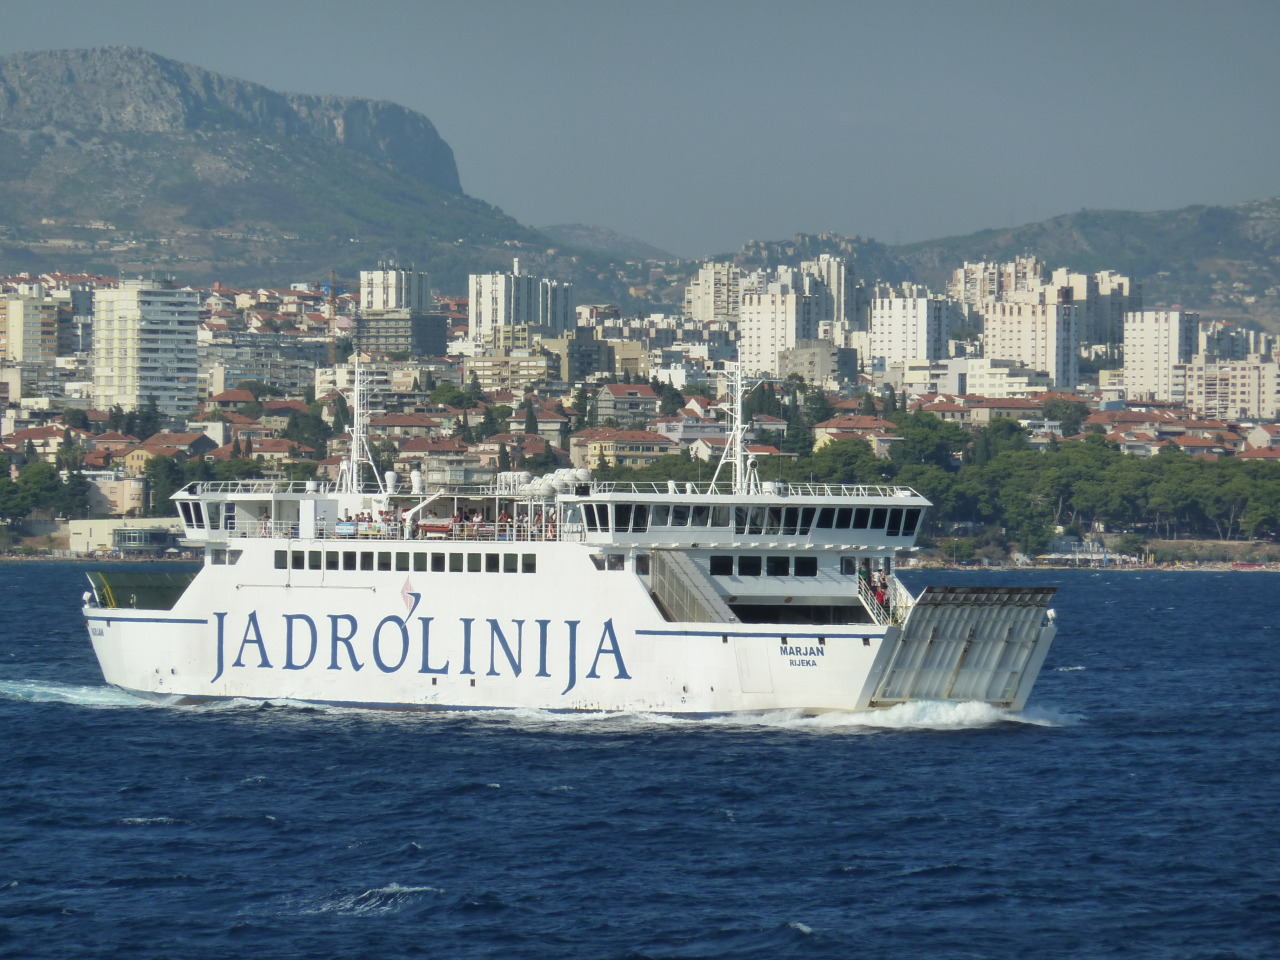
\includegraphics[width=0.4\textwidth, height=5cm, keepaspectratio]{../Bilder/Sommer2012/76.jpg}
    \caption{Fähre}
  \end{centering}
\end{wrapfigure} 

Split war in Sicht und mit der Stadt auch die Tafelberg ähnlichen Erhöhungen im Hintergrund.
Was zusätzlich auffiel, war die Verfärbung der Luft, hervorgerufen durch etliche Feuer rund um Split.
Seit längerer Zeit waren wieder einmal Hochhäuser in Sicht und wir beschlossen, dass wir Split nicht näher anschauen wollten und gleich Richtung Trogir weiterziehen wollen.
Dort angekommen war der erste aufgesuchte Camping in Stadtnähe leider voll.
Es wies jedoch ein Schild auf einen anderen hin, denn wir sogleich aufsuchten.
2 km vor dem Camping war es dann vorbei mit Teerstrasse und ein unbefestigter Weg breitete sich vor uns aus.
Los ging die wilde Fahrt, welche durch einen winzig kleinen sehr freundlichen Campingplatz mit angeschlossenem Restaurant belohnt wurde.
Der Stellplatz war zwar selbst für unseren kleinen Bus sehr eng, jedoch mit direkter Sicht auf das Meer.
Zum Abendessen gab es Dalmatinischer Rohschinken und je 300 gr. Scampi mit Pommes Frites.
Herrlich.
Danach fiel ich müde ins Bett, während Chantal noch kurz die Berichte auf Vordermann brachte.

\subsection{19.08.2012 Strandtag}

\begin{wrapfigure}{R}{0.45\textwidth} 
  \begin{centering}
    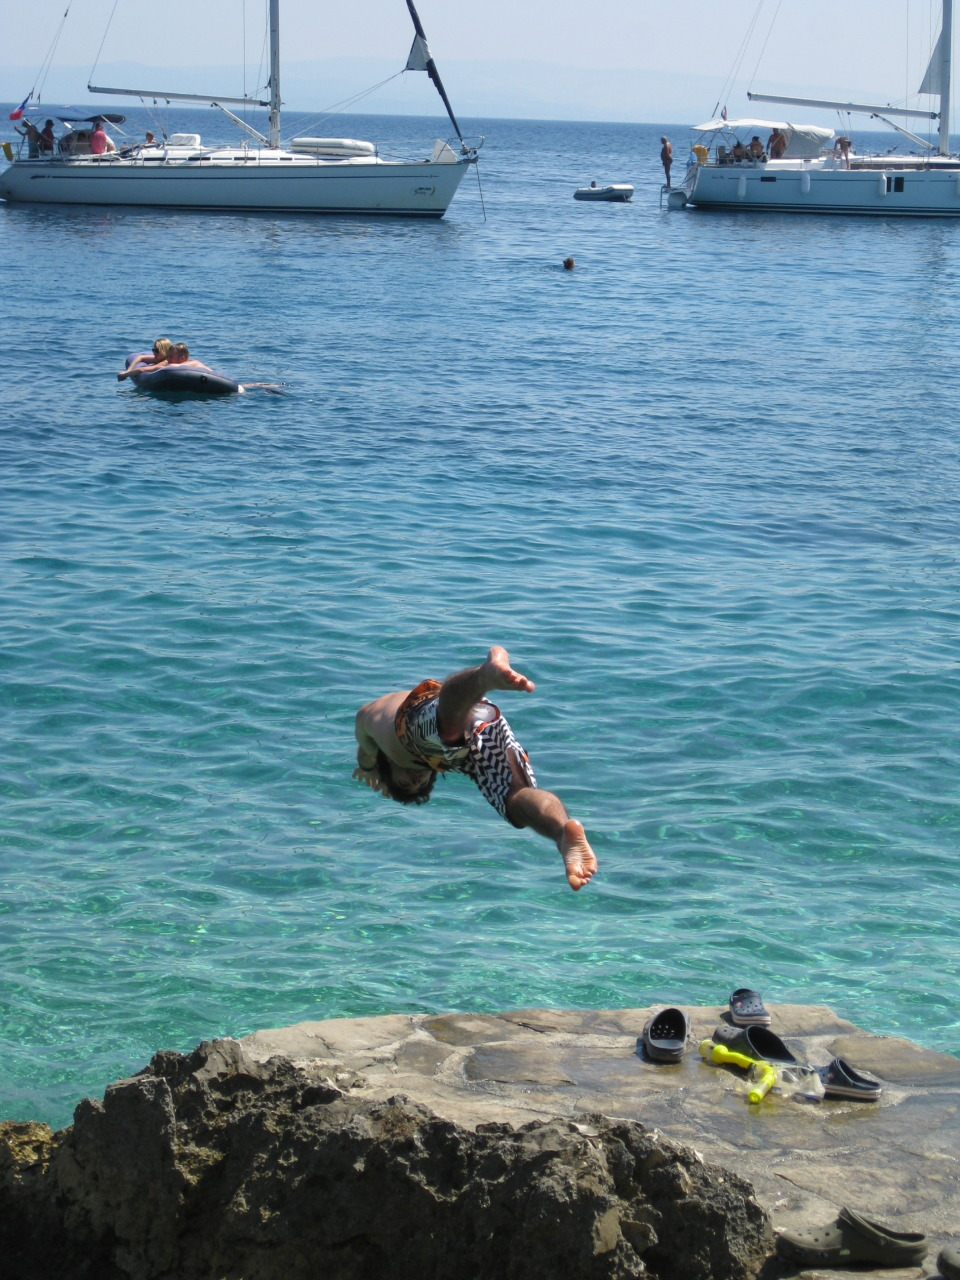
\includegraphics[width=0.4\textwidth, height=5cm, keepaspectratio]{../Bilder/Sommer2012/78.jpg}
    \caption{Kühles Nass}
  \end{centering}
\end{wrapfigure} 

Um kurz nach acht trieben uns die schon stark erhöhte Temperatur und das Brot das von 8-9 verkauft wird aus den Federn.
Chantal besorgte uns ein reichlich gedeckter Frühstückstisch.
Ein kurzer Ausflug unter die Dusche und bald schon stand der sehr kurze Spaziergang zum Strand an.
Das wunderbar klare Wasser und die hohen Temperaturen verfehlten ihre Wirkung nicht und schon bald schwammen wir mit Go Pro, Schnorchel und Taucherbrille in der herrlichen Bucht.
Dösen und Lesen ergaben dann schnell Hunger und das Restaurant, welches uns am Vorabend mit Essen versorgte versuchte mit Scampis über dem Feuer gebraten die Gäste zu verführen.
Wie unschwer zu erraten ist funktionierte diese List bei uns perferkt und nur vom Unterbewusstsein gesteuert fanden wir uns vor dampfenden Nudeln mit Scampis wieder.
Eigentlich wollten wir wenn möglich noch Trogir besichtigen, was jedoch dank des schönen Strandes eher morgen geschehen wird.

Wie man leicht erkennen kann, eignen sich Strandtage nicht gerade dazu viel und interessantes zu berichten.
Vielleicht noch dass: Unser Cola-Flaschen-Wein hat die warme überfahrt in der Fähre nicht gut überstanden.
Der Geschmack hat sich zwar nicht verändert, die Auswirkungen hingegen schon.

\begin{figure}[H]
    \centering
    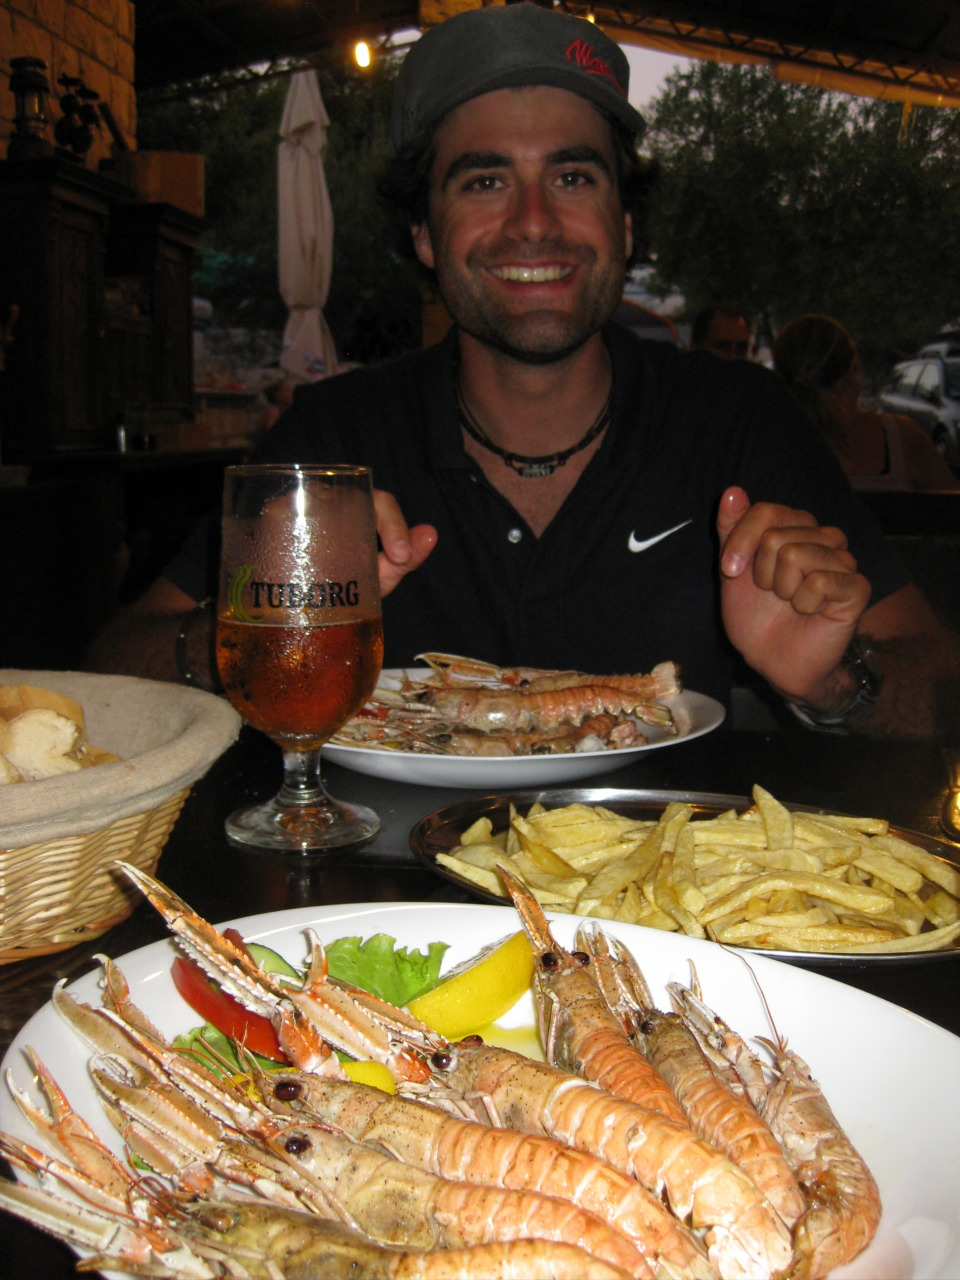
\includegraphics[width=0.4\textwidth]{../Bilder/Sommer2012/77.jpg}
    \caption{Abendessen}
    \label{img:Sommer9}
\end{figure}


\subsection{20.08.2012 Fahrt über eine total andere Insel}
Wir werden die wunderschöne Aussicht, welche jedes Morgenessen hier untermalt vermissen.
Trotzdem hiess es heute weiter ziehen Richtung Norden.
Auch diese Frühstück wurde durch feine Bäckerei-Leckerbissen aufgemöbelt.
Dieses Mal war es ein Apfelstrudel und zwei Berliner (einer mit Nutella, Gruss an Susi).
Bevor wir nach Trogir reinfahren konnten, mussten wir noch etliche Hürden überwinden.
Zuerst mussten wir den schmalen Weg meistern.
Chantals Abdrücke der Fingernägel sind immernoch am "Angsthasengriff" sichtbar.
Als zweites mussten wir einkaufen, überhaupt kein Problem, da ein Market auf dem Weg lag.
Das dritte Problem bestand darin, nach Trogir zu kommen.
Das malerisch gelegene Städtchen bietet die einzige Brücke zu der Insel, auf der wir uns befanden.
Entsprechend beliebt ist dieser Ort bei den Autofahrern.
Nach etwa einer Stunde Stop and Go haben wir die zwei Brücken erreicht und fanden noch kurz Zeit mit einem Schweizer Ehepaar zu quatschen, welche sich über Jack freuten.
Ein Parkplatz war dann schnell gefunden und auf ging es die Stadt und Ihre Schmuckgeschäfte zu erkunden.
Eine wunderschön gelegene Stadt, die jedoch irgendwie wie jede andere kroatische Stadt aussah, die wir bis anhin besuchten.
Massen von Touristen wuselten durch die Gassen und die ganze Altstadt bestand aus Restaurants.
Nach einer feinen Pizza ging es Richtung Norden.

\begin{figure}[H]
   \centering
      %\subfloat[CAPTION]{BILDERCODE}\qquad
   \subfloat{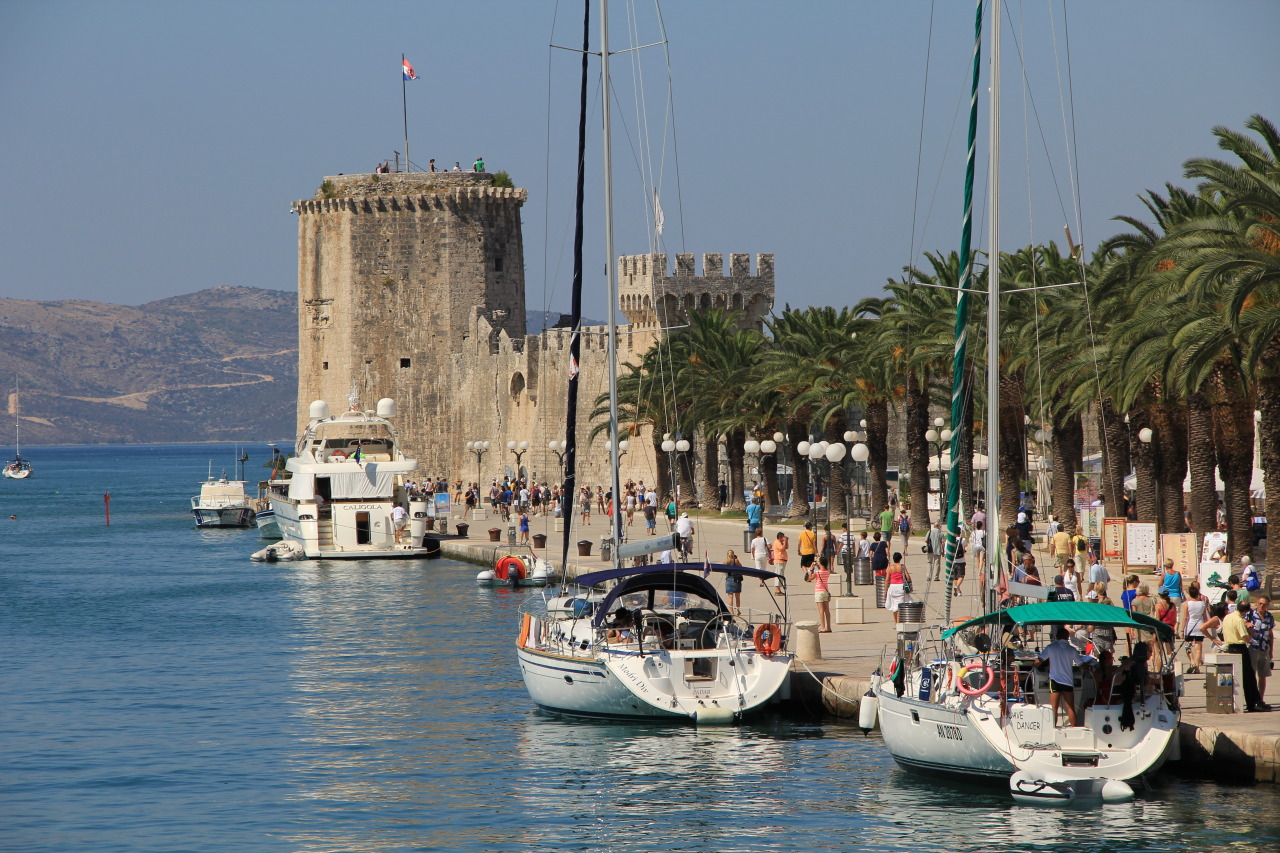
\includegraphics [width=0.3\textwidth]{../Bilder/Sommer2012/80.jpg}}\quad
   \subfloat{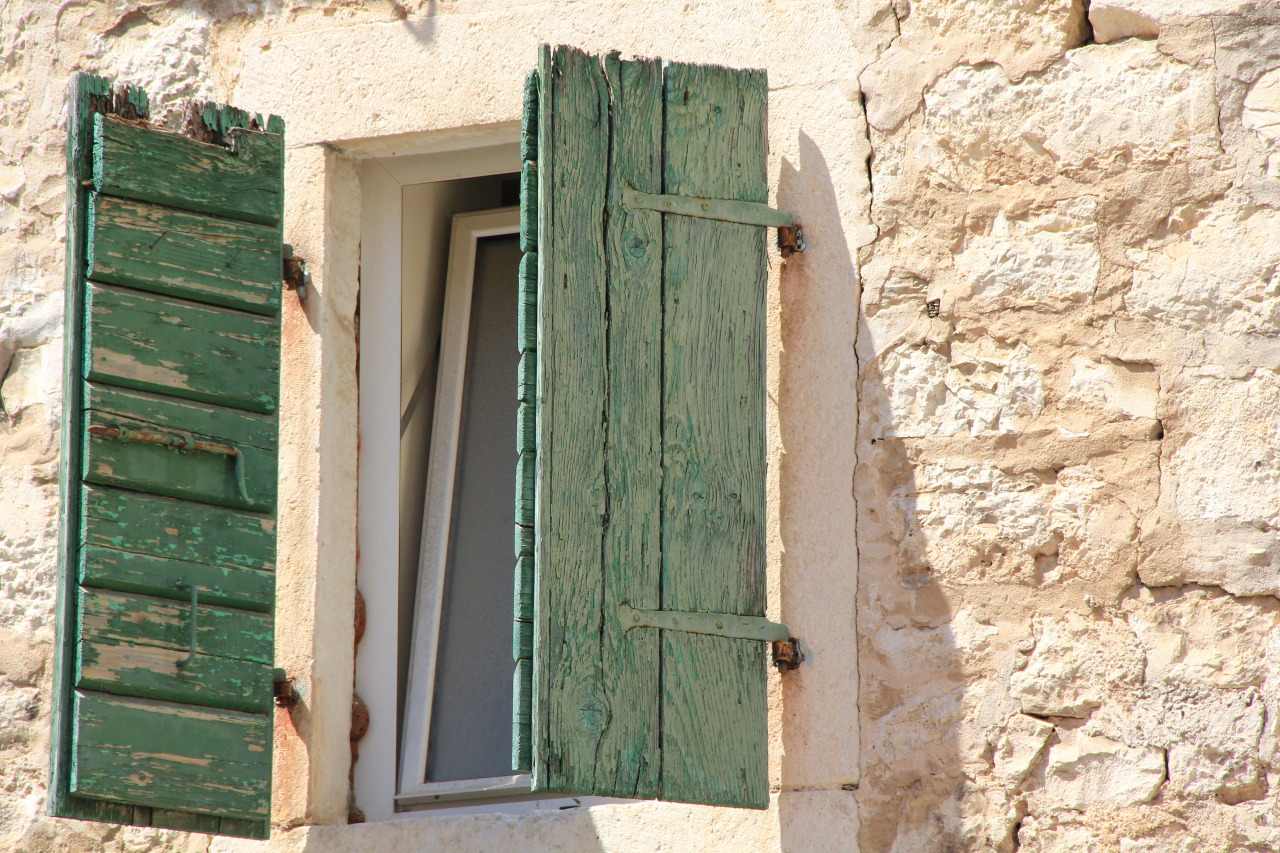
\includegraphics [width=0.3\textwidth]{../Bilder/Sommer2012/81.jpg}}\quad
   \subfloat{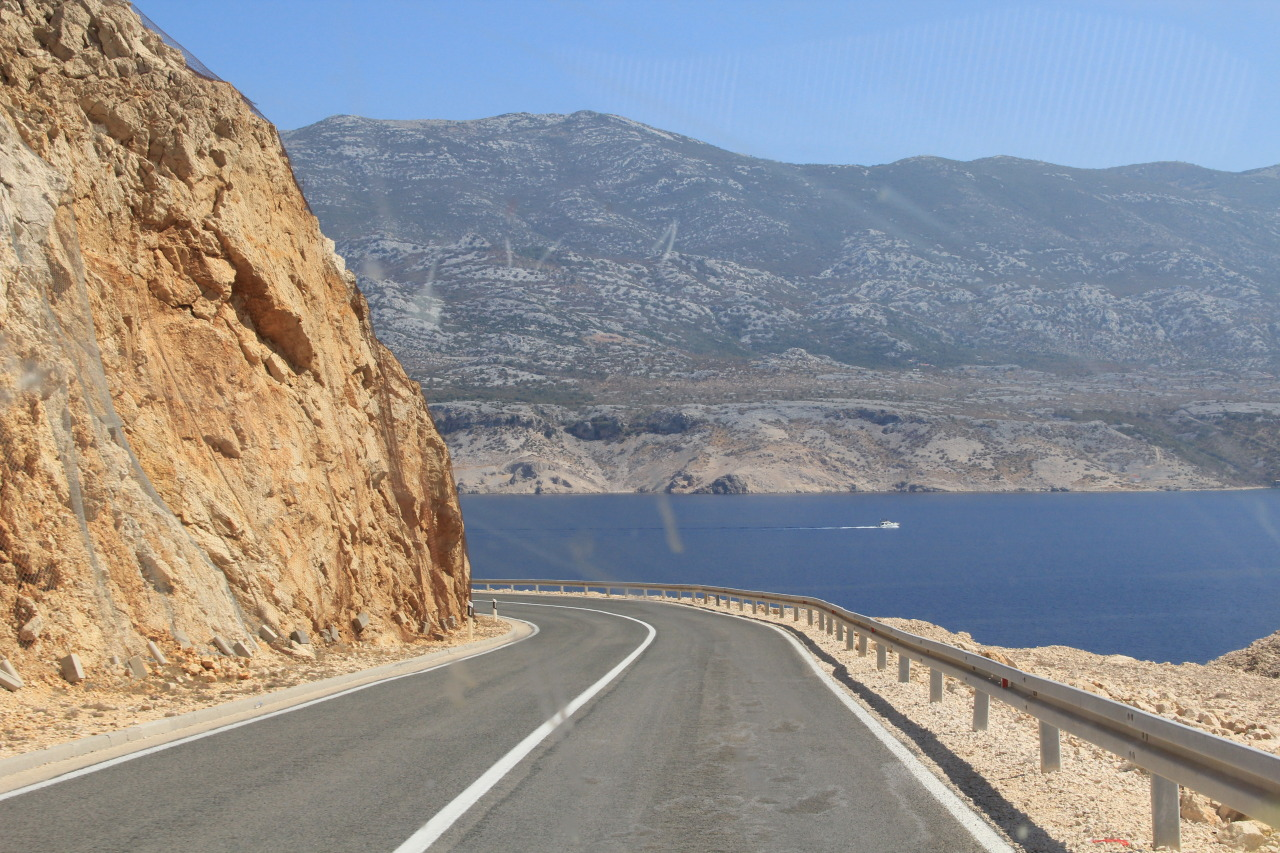
\includegraphics [width=0.3\textwidth]{../Bilder/Sommer2012/86.jpg}}\quad
   \caption[Trogir]{Trogir}
\end{figure}

Kurz vor der Autobahnauffahrt überholten uns wieder einmal Löschflugzeuge um in Sisiphusarbeit den nahe brennenden Wald zu löschen.
Überhaupt sieht man sehr viele schwarze, runtergebrannte Stellen wenn man durch diese sehr trockene Gegend fährt.
Das Bezahlsystem funktioniert sehr ähnlich wie das in Italien, nur moderner schneller und freundlicher.
Auch das Chaos nach der Bezahlstelle hält sich stark in Grenzen.
Es fuhren im allgemeinen nur wenige Fahrzeuge auf der gut ausgebauten Autobahn.
Die Vegetation änderte sich schlagartig, als wir auf die Insel Pag auffuhren.
Nix mehr Grünes, es war eher eine Mondlandschaft als das bekannte Inselartige, dass uns jetzt schon über eine Woche begleitete.
Das herrlich blaue Wasser bildet einen wunderbaren Kontrast zu den hellen steinigen Weiten.

Unser erster angesteuerte Campingplatz lag ganz am Ende der Insel und gegen Ende eben dieser wurde die Strasse immer spannender mit Kuppen überzogen die dem Fahrer grosse Freude bereiteten.
Auch dieser Platz lag wieder wunderschön an einer einsamen Bucht und am Ende einer engen Strasse.
Als wir dem Platz entlang fuhren, wurde uns jedoch schnell klar, dass hier nichts mehr zu machen ist.
Voll.
Leider bestätigte sich dieser Verdacht und der nahegelegene Alternativplatz bot leider weit und breit
keine Verpflegungsmöglichkeit, geschweige denn Elektrizität.
Also fuhren wir auf dem Inselrücken zurück nach Novalja, wo sich einer der Top 10 Plätze Kroatiens befinden soll.
Der Platz ist gigantisch.
Über 1200 Stellplätze eigene Check in Spur in der Anfahrtsstrasse, Sportcenter und und und... Wir waren zuerst nicht gerade begeistert, jedoch mussten wir unsere Meinung sehr schnell ändern.
Schöner Strand, sehr schöne Sanitäre Anlagen, alles passt.
Nach dem wir wieder einmal selber gekocht hatten
(Sweet \& Sour mit Reis und Poulet, dazu Maissalat) fielen wir Müde aber glücklich ins Näscht.
Da wir auf dieser Reise einen GPS Tracker mitführen kennen wir ausnahmsweise (ein kleines Leiden von Jack) die zurückgelegten Kilometer.
Wir haben bis zum heutigen Tag 2245 km zurückgelegt.
Ohne auf Probleme gestossen zu sein.
Wir hoffen, dass es auch auf dem Rest der Reise so bleiben wird.

\begin{figure}[H]
   \centering
      %\subfloat[CAPTION]{BILDERCODE}\qquad
   \subfloat{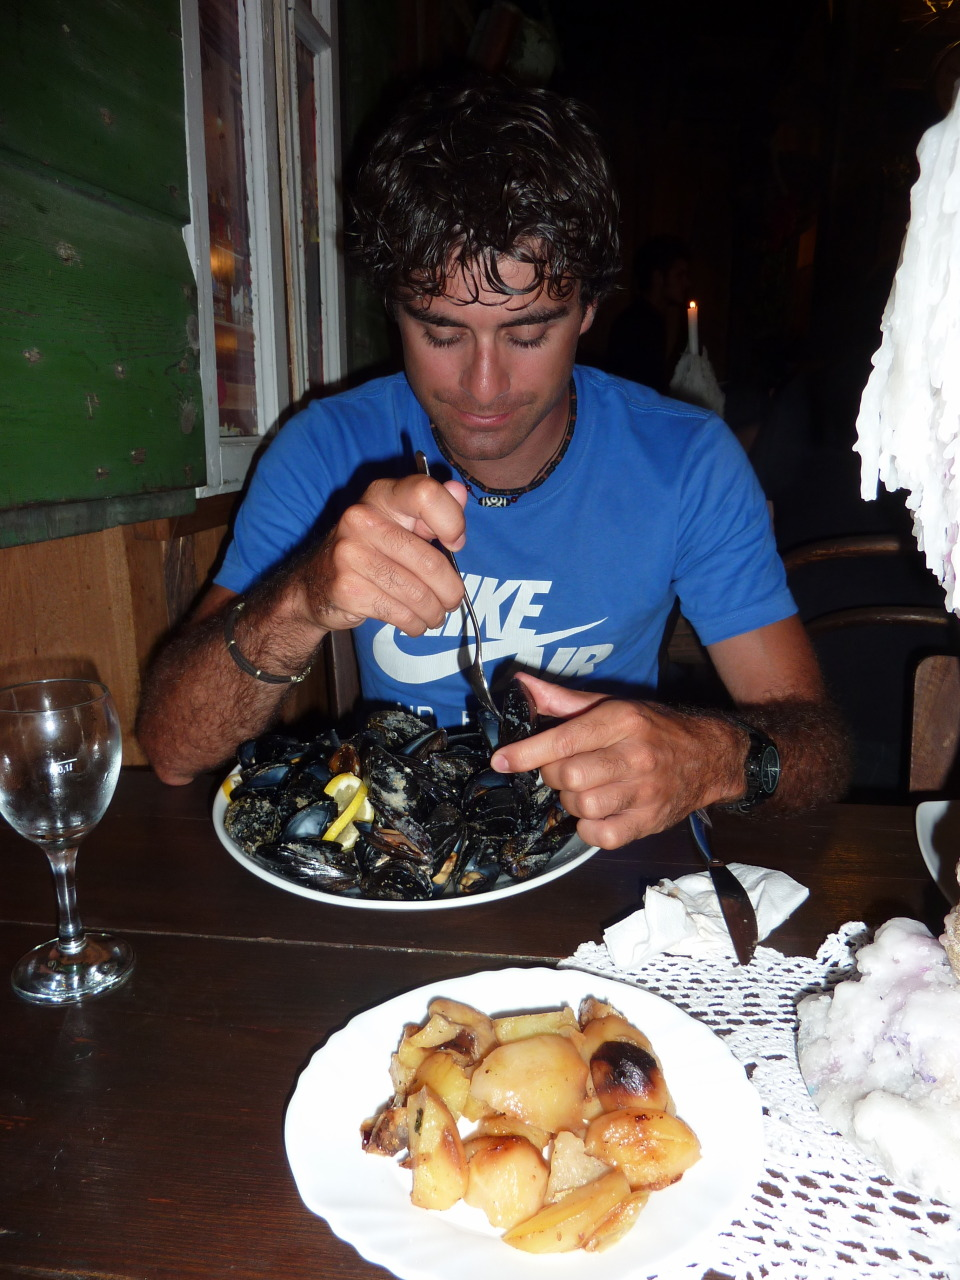
\includegraphics [width=0.3\textwidth]{../Bilder/Sommer2012/83.jpg}}\quad
   \subfloat{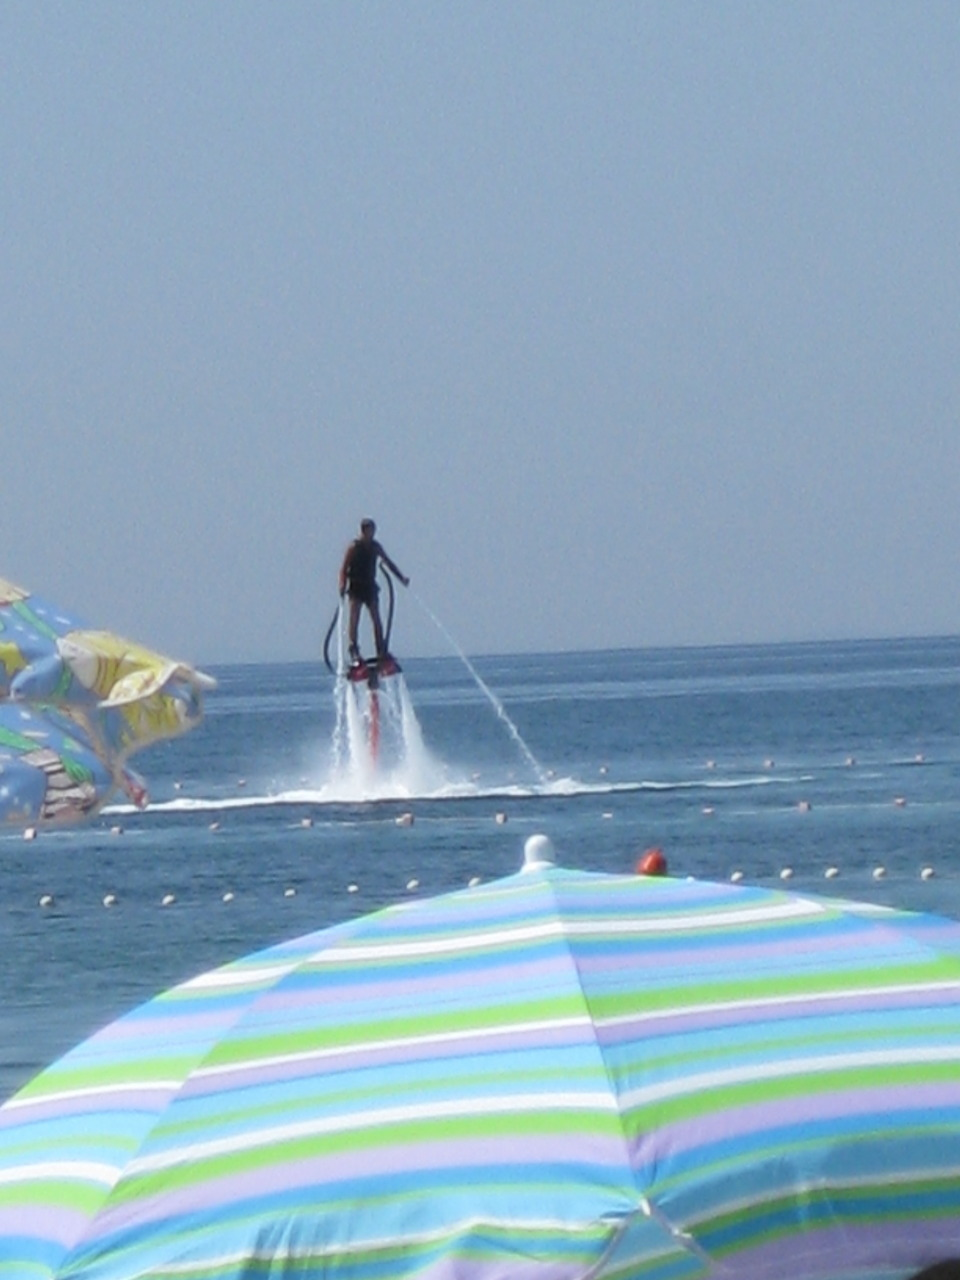
\includegraphics [width=0.3\textwidth]{../Bilder/Sommer2012/82.jpg}}\quad
   \subfloat{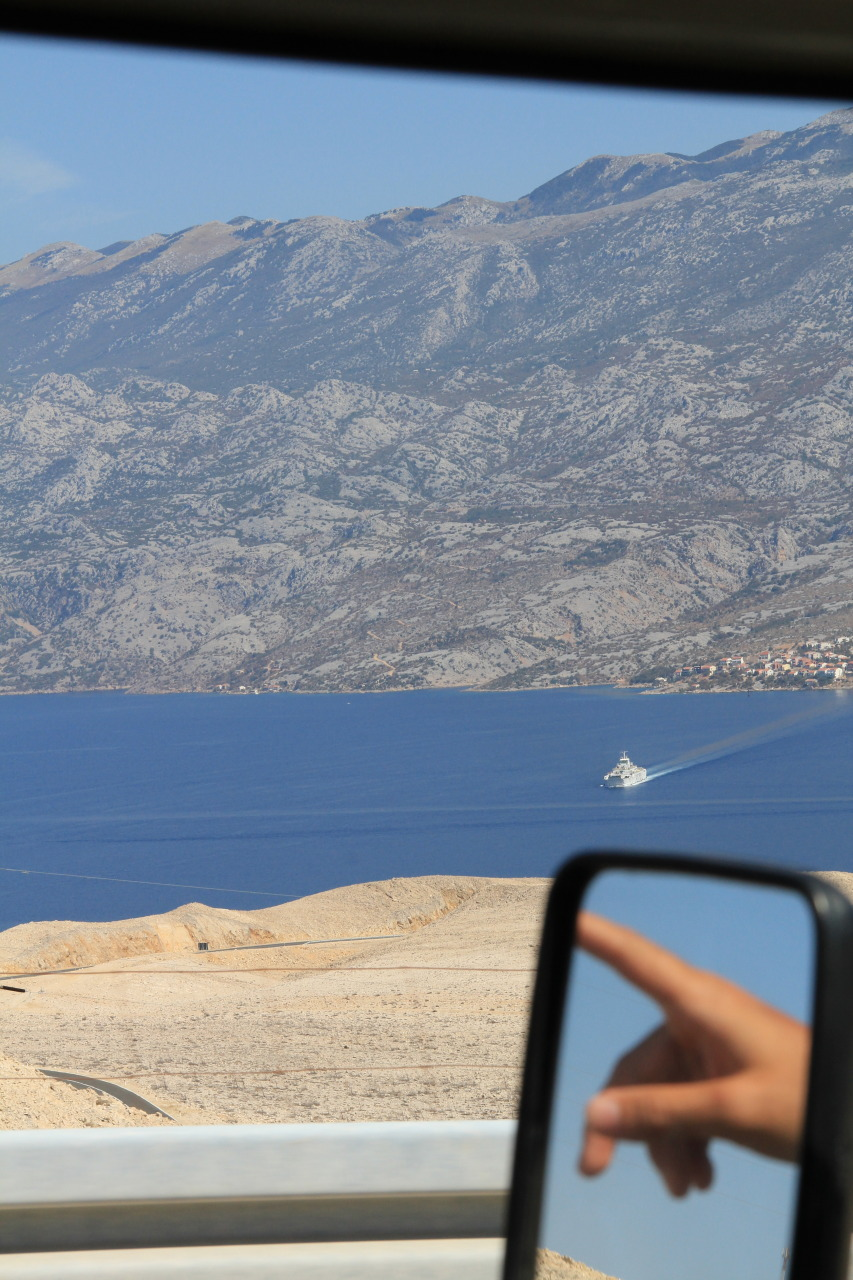
\includegraphics [width=0.3\textwidth]{../Bilder/Sommer2012/85.jpg}}\quad
   \caption[Pag]{Pag}
\end{figure}

\subsection{21.08.2012 Annehmlichkeiten eines Luxus-Campingplatzes}
Tagwach verschliefen wir gekonnt.
So standen wir erst gegen 10:00 auf, was wir auch unserem schattigen Plätzchen verdanken konnten.
Danach ging ich einkaufen und besorgte das Passwort für das streng geschützte Platz eigene WLAN.
Damit konnten wir uns wiedereinmal über die geschehenen Dinge in der Welt informieren und Chantal bekam die wunderbare Nachricht, dass sie die nächste Zeit viel Spass an der Französischen Sprache haben darf.
Als die Sonne ihren höchsten Stand erreichte begaben wir uns an den Strand.
Dieser war wie alles auf diesem Platz einfach gigantisch.
Jede erdenkliche Wassersportart wurde angeboten, bis zum Wasserstrahl betriebenen Raketenrucksack.

Als wir eine feine Garstufe erreicht hatten, war es Apérozeit und danach wurden die Duschen aufgesucht.
Die Fahrt an den endlosen Caravan-Stellplätzen vorbei war eindrücklich und wenig später kam schon das Dörfchen direkt am Wasser ins Sicht.
Am Eingang zum Dorf warteten schon die Restaurants mit montierten Spanferkel auf die zahlende Kundschaft.
Das ausgesuchte Restaurant konnte vollends überzeugen.
Auf dem Weg dorthin war ich mir noch sicher heute garantiert kein Fisch zu essen.
Dieser Vorsatz verschwand dann aber schneller als er aufgetaucht war beim Blick auf die Speisekarte.
Schlussendlich fanden Miesmuscheln und Risotto mit Meeresfrüchten ein weiteres Mal den Weg auf den Tisch.
Chantal verschonte die überfischten Gewässer mit ihrer Wahl und suchte sich Teigwaren mit Trüffel aus.
Nach dem Essen war auf der Strandpromenade dir Party voll im Gange und auch die Geschäfte lockten Chantal ein weiteres Mal mit ihren hochwertigen Artikel an.
Auf dem Zeltplatz angekommen herrschte auch da in einem der vielen Restaurants noch Oktoberfeststimmung.
Bald darauf legten wir uns auf die Ohren und hörten für die nächsten Stunden dem Kopfkissen zu.

\subsection{22.08.2012 Rab - Zeit um die Insel zu wechseln}
Heute wollten wir Dea und Lukas besuchen.
Deas Familie besitzt eine wunderschöne Ferienwohnung oberhalb von Rab mit einem atemberaubenden Ausblick über das Städtchen.
Zuerst mussten wir jedoch von Novalja auf Pag zurück auf das Festland um dann wiederum auf die nächste Insel, eben Rab zu kommen.
Kurz vor zwölf machten wir uns auf den Weg und weil beide benötigten Fähren im 20 min Takt fuhren kamen wir kurz darauf schon in Rab an.
Eigentlich haben wir uns für etwa 18:00 Uhr angemeldet und die beiden genossen noch das glasklare Wasser auf der Insel Frkanj.
Chantal besorgte die Geschenke für Silas (ihr Göttibueb) und ich versuchte Impressionen mittels Fotoapparat auf die Harddisk zu schreiben.
Der kleine Hunger meldete sich, hatte jedoch auch hier kaum eine Chance gegen die Flut der Restaurants.
Es war höchste Zeit sich mit Hilfe des Wassers abzukühlen.
Rab besitzt auf der einen Seite eine wunderschöne Uferpromenade, welche zum Baden einlädt. Kaum dort angekommen und die ersten Krebse
und Fische beobachtet meldeten sich unsere beiden Gastgeber, dass sie auf dem Rückweg von der kleinen Insel seien.
Wir trafen die beiden im Hafen und beschlossen die Abendsonne am vorher besuchten Stadtstrand zu geniessen und erst nachher mit Jack zur besagten Wohnung zu fahren.
Der Weg da rauf war steil und eng und die beiden organisierten gar extra einen Parkplatz für den Bus.
Wir durften ein eigenes Zimmer beziehen mit eigenem Bad.
Welch Luxus nach fast drei Wochen Camping.
Dea hatte natürlich ein paar gute Vorschläge für das Nachtessen und dank ihrem kroatisch verschwanden schnurstracks die \glqq Reserviert \grqq Täfelchen von den letzten Tischen im Restaurant und wir genossen ein herrliches Abendessen zu viert.

\begin{figure}[H]
   \centering
      %\subfloat[CAPTION]{BILDERCODE}\qquad
   \subfloat{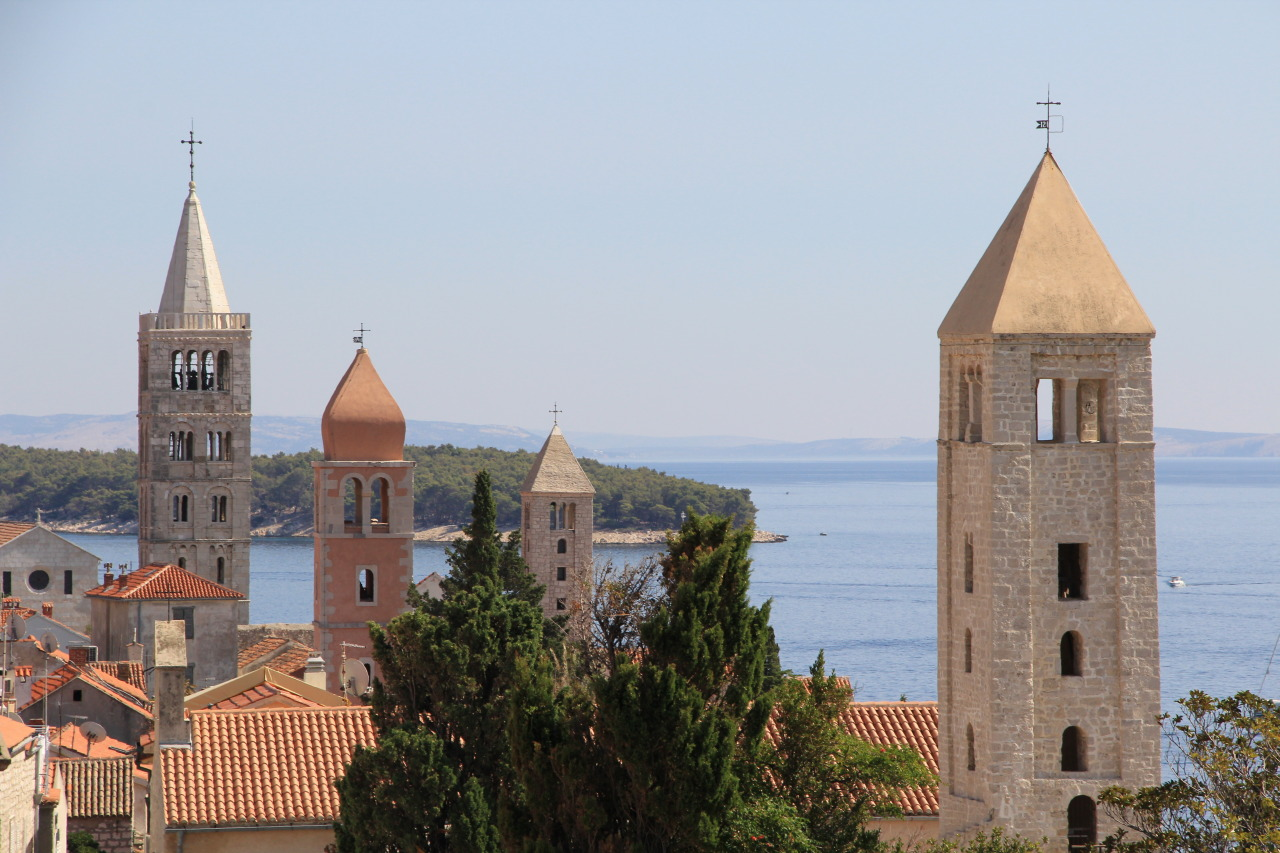
\includegraphics [width=0.3\textwidth]{../Bilder/Sommer2012/94.jpg}}\quad
   \subfloat{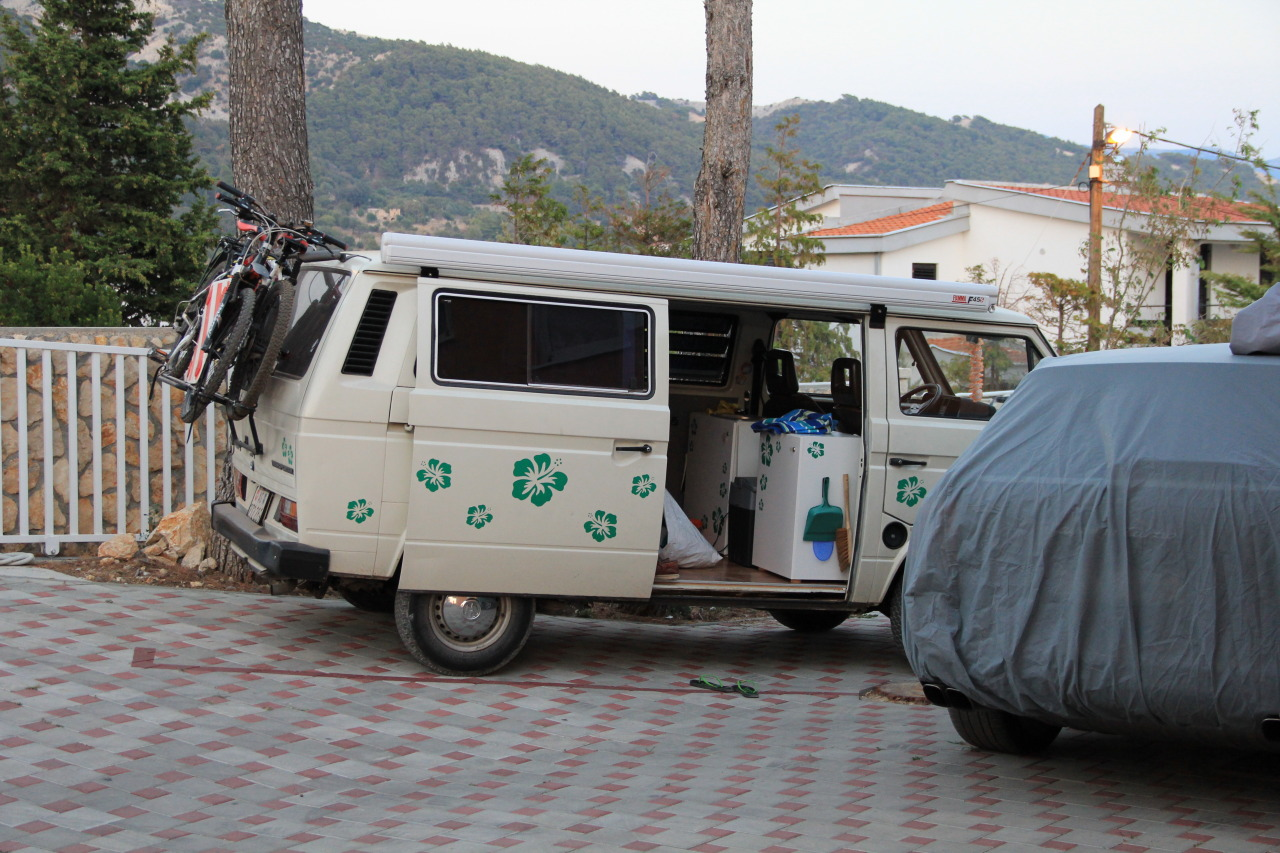
\includegraphics [width=0.3\textwidth]{../Bilder/Sommer2012/98.jpg}}\quad
   \subfloat{\includegraphics [width=0.3\textwidth]{../Bilder/Sommer2012/99.jpg}}\quad
   \caption[Besuch bei Freunden]{Besuch bei Freunden}
\end{figure}

\subsection{23.08.2012 Die Liebesinsel ;)}

\begin{wrapfigure}{L}{0.45\textwidth} 
  \begin{centering}
    \includegraphics[width=0.4\textwidth, height=5cm, keepaspectratio]{../Bilder/Sommer2012/100.jpg}
    \caption{Steinmannli}
  \end{centering}
\end{wrapfigure} 

Wieder einmal ein richtiges Bett, juhuu :) Wir kamen fast nicht aus den Federn, als um 8 Uhr der Wecker klingelte.
Und dies obwohl uns schon um 6 Uhr ein Geräusch weckte; kiikerikiii, kikerikii.
Kaum aufgestanden, war schon das Frühstück parat: feine Müesli, Brot, Marmelade, Wassermelone...alles was das Herz begehrte, hmm:).
Und all dies konnten wir mit einer herrliche Aussicht auf Rab und vorgelagerten Inselchen geniessen.
Eine dieser Inseln war die Insel Frkanj, die sogenannte Liebesinsel; welche wir heute besuchen wollten.
Nach dem gemütlichen Frühstück packten wir unsere Standsachen und machten uns auf den Weg zum Hafen.  Dort wartete schon unser Taxiboat.
Die Fahrt nach Frankj war herrlich und dort angekommen, wussten wir, dass es noch viel herrlicher wird:) Glasklares Wasser, einen schönen Pinienwald und ein super Restaurant erstreckten sich vor uns.
Wir suchten uns ein lauschiges Plätzchen im Schatten aus und machten schon bald ein Sprung ins Wasser...wow, wunderschön wares! Den Rest des Tages verbrachten wir mit: schwimmen, schnorcheln, faulenzen, spektakuläten Steinmännli bauen (gäll Steff:)) und essen.
Zu Mittagessen gab es feine Meeresfrüchte und Fleisch (niemand traute sich an das Spannferkel).
Auch diesmal bekamen wir dank Dea einen eigentlich reservierten Spitzenplatz.
Nach dem Essen verfielen wir in einen Tiefschlaf.
Doch wir konnten uns dann doch noch aufraffen für einen weiteren Schwimmtrip zum Restaurant und für einen Misch-masch und Sonnenaufgang, welcher sich dann leider als Sonnenuntergang herausstellte.
Das Taxiboat zurück haben wir knapp noch erwischt.
Im Hafen angekommen, waren wir alle ein bischen plemplem und schlenderten den Hang hinauf zu Deas Wohnung.
Dort ging es ruckzuckzackzack ans Kochen und schon bald konnten wir ein feines Nachtessen mit Spaghetti, serbischem Salat und sehr sehr gutem Wein mit wunderschöner Aussicht geniessen.
Die farbige Disco-Beleuchtung zog uns dann noch zur down town von Rab;) Nach einem Stadtrundgang entschieden wir uns schließlich für eine Bar, wo es Mojito, Wasser und Eistee gab (jemand hatte schon zu viel von dem guten Wein getrunken;)).
Es war ein gelungener Ausklang für einen wunderschönen Tag!

\begin{figure}[H]
    \centering
    \includegraphics[width=\textwidth]{../Bilder/Sommer2012/102.jpg}
    \caption{Sonnenuntergang}
    \label{img:Sommer10}
\end{figure}

\subsection{24.08.2012 Wir müssen weiterziehen}
Auch wenn es noch so schön auf Rab gewesen ist, war trotzdem die Zeite gekommen um weiterzuziehen.
Dea und Lukas entschieden sich die Gelegenheit für eine Besuch der Strände um Lopar.
Wir parkten den Bus vor dem Fährehafen und wollten eigentlich gleich Tickets für die Fähre kaufen.
Das Ticket-Office öffnete seine Fenster jedoch erst um 13:00.
Der Bus stand jedenfalls so nahe an der Poleposition wie noch nie, was einem garantierten Platz auf der Fähre gleichkommt.
Mit dem Fahrzeug der beiden ging es dann auf Strandsuche.
Nach kurzer Fahrt empfing uns ein Parkticketverkäufer im weiten Wald.
Dieser wollte Geld für ein Ticket, welches die Einfahrt in seinen Parkplatz ermöglicht.
Es war nicht gerade ein Parkplatz im klassischen Sinne.
Viel eher ein bewaldetes Stück Land, durchzogen von etlichen Strassen und Wege, an denen sich überall Ecken und Plätzchen für das Abstellen der Fahrzeuge finden lies.
Um an den Strand zu gelangen war dann ein längerer Marsch notwendig und wir fürchteten uns schon vor möglichen Nakedei, die an diesen Strandabschnitten geduldet wurden.
Nach den ersten vorsichtigen Blicken gab es Entwarnung und wir trauten uns näher an die Bucht, welche durch grelles Kindergeschrei mit Leben erfüllt worden ist.
Die ziemlich grosse Bucht bot die Möglichkeit 200 Meter über feinsten Sandboden ins Meer heraus zu waten ohne das der Nauchbabel auch nur in die Nähe der Wasseroberfläche gekommen wäre.
Leider war das Ufer jedoch nur etwas für hartgesottene Sonnenanbeter.
Trotzdem lies ich es mir trotz einiger Grillbratwurst-Präsentierer nicht nehmen und sprang kurz ins Wasser.
Ganz zur Freude von Chantal.
Danach mussten die leeren Batterien und Fettreserven wieder aufgefüllt werden, was wir in einem nahegelegenen Restaurant genüsslich taten.
Dann war es an der Zeit Abschied zu nehmen um die Tickets für die Fähre zu kaufen, welche laut Fahrplan um 14:00 abfahren sollte.
Wir hatten noch über eine Stunde Zeit.
Die Kaffeemaschine wurde angeworfen um die Wartezeit zu verkürzen.
Immer noch keine Fähre in Sicht.
Auch um 15:00 keine Spur einer Fähre.
Wir beschlossen ein letztes Bad auf der Insel Rab zu nehmen und holten unsere Badesachen.
Genau in diesem Moment tuckerte die sehr behäbig scheinende Fähre in den Hafen, wo umgehend damit begonnen wurde Fahrzeuge abzuladen.
Gespanne mussten Rückwärts von der Fähre fahren und das Ganze schien einmal nicht ganz so reibungslos abzulaufen wie sonst gewohnt.
Als wir Jack auf der Fähre platziert hatten und einen Platz im Innern der Fähre eingenommen hatten, setzte sich das Schiff in Bewegung.
Nach gut 1 ½ Stunden sollten wir eigenltich auf Krk ankommen doch wir waren noch weit vom Hafen entfernt.
Es war fast Windstill auf Deck und das Schiff schien sich doch sehr langsam fortzubewegen.
Eine Messung mit GPS ergab bescheidene 15 km/h.
Mit über ¾ Stunden Verspätung obendrauf liefen wir in den Hafen ein.
Krochen wäre der bessere Ausdruck dafür.
Das schiff wollte irgendwie nicht mehr so recht und auch die wilde Huperei unseres Kapitäns verbesserte die Situation nicht.

\begin{figure}[H]
   \centering
      %\subfloat[CAPTION]{BILDERCODE}\qquad
   \subfloat{\includegraphics [width=0.3\textwidth]{../Bilder/Sommer2012/89.jpg}}\quad
   \subfloat{\includegraphics [width=0.3\textwidth]{../Bilder/Sommer2012/90.jpg}}\quad
   \subfloat{\includegraphics [width=0.3\textwidth]{../Bilder/Sommer2012/87.jpg}}\quad
   \caption[Warten auf die Fähre]{Warten auf die Fähre}
\end{figure}

Wir folgten der Strasse auf Krk Richtung Norden und mussten uns immer noch entscheiden wie die nächsten Tage aussehen werden.
Verona war noch eine Wunschdestination von Chantal und so beschlossen wir Kroatien schon heute zu verlassen und möglichst nahe an Verona heranzufahren und die Ferien dann im Südtirol ausklingen zu lassen.
Neuigkeiten aus Stans und ein Besuch aus dem hohen Norden bekräftigte unsere Entscheidung unsere Reise ein wenig zu Beschleunigen.
Nach einem Halt an einer Raststätte,
wo es auch die Möglichkeit gab endlich das klebrige Salz loszuwerden.
Seit langer Zeit war auch wieder einmal Zeit einen Mc Donald's aufzusuchen.
Die Fahrt dauerte noch bis kurz vor 24:00 Uhr und gut 70 km vor Verona.

\subsection{25.08.2012 Shopping-Rausch in Verona}

\begin{wrapfigure}{L}{0.45\textwidth} 
  \begin{centering}
    \includegraphics[width=0.4\textwidth, height=5cm, keepaspectratio]{../Bilder/Sommer2012/105.jpg}
    \caption{Panne kurz vor dem Ende der Reise}
  \end{centering}
\end{wrapfigure} 

Kurz vor dem Kalterersee musste ich ein ungewohntes Geräusch feststellen, welches jedoch zuerst einmal ignoriert wurde.
Eine Minute später zog jedoch ein unschöner Geruch durch unseren Bus.
Ich erwähnte noch das es nach Gummi rieche und schon sah ich im Rückspiegel die Luft aus unserem hinteren linken Reifen entfleuchen.
Ab auf den Pannenstreifen und den Schaden zu begutachten.
Vibrationen haben das Ventil des alten Pneus dazu bewogen sich vom Gummi zu verabschieden.
aus diesem Riss strömte jetzt die kostbare Luft aus.
Warnweste, Pannendreieck, Wagenheber und Reservepneu behoben die Situation jedoch in 20 Minuten.
Einzig das ungute Gefühl blieb, dass ein weiterer solcher Vorfall die Reise definitv zum erliegen bringen könnte.

Am See angekommen wurde uns relativ schnell klar, dass ich die Situation unterschätzt hatte.
Platz war nirgends mehr frei.
Nicht in Hotels und schon gar nicht auf den Zeltplätzen.
Wir beschlossen bis nach Bozen weiterzufahren und dort unser Glück zu versuchen.

Tatsächlich fanden wir nach kurzer Suche ein Hotel für einen angemessenen Preis und konnten den Bus sogar noch zum Schutz vor dem aufkommenden Gewitter in eine (höhere) Tiefgarage stellen.

Nach einer eher unruhigen Nacht auf der Autobahnraststätte, machten wir uns nach einem Kaffee auf den Weg die letzten 70 kam nach Verona zurückzulegen.
Kaum in Verona angekommen ging die Suche nach einem geeigneten Parkplatz los.
Ab ins Zentrum und schon standen wir vor einem Parkhaus.
Die Höhenlimite von 2.15m machte uns jedoch einen Strich durch die Rechnung.
Nach genauer begutachtung durch Chantal (Mit klassischen Meinungsänderungen alle 30 cm, beim heranrollen an den Balken) stand dann fest wir passen nicht da rein.
Alles zurück.
Natürlich stand der nächste potentielle Parkeur schon hinter uns und musste auch zurücksetzen.
Nebenan gab es glücklicherwiese einen nicht überdachten Parkplatz, welchen wir für ein beträchtliches Entgelt benutzten durften.
Die Stadt war gut gefüllt mit Schweizer Shoppingtouristen und auch wir machten keine Ausnahme und erfüllten unsere Pflicht, der EU finanziell unter die Arme zu greifen.
Wir schlenderten lange, trotz hohen Temperaturen, durch die schöne Stadt und machten uns erst gegen 18:00 auf den Weg Richtung Norden um unser Tagesziel zu erreichen.
Das Südtirol. 

\begin{figure}[H]
    \centering
    \includegraphics[width=\textwidth]{../Bilder/Sommer2012/103.jpg}
    \caption{Verona}
    \label{img:Sommer11}
\end{figure}

\subsection{26.08.2012 der letzte Tag}

Nun ist er angebrochen, der letzte Tag der Reise.
Das Wetter zeigte sich von seiner trüben Seite, welche uns jedoch für die letzten Kilometer entgegen kam.
Nach einem ausgiebigem Frühstück legten wir los und fuhren die Strecke bis nach Arbon ziemlich direkt durch.
Dort wollten wir am See das letzte Essen unserer Reise geniessen.
Arbon war voll Velofahrern da gerade Slow up war.
Das Wetter begrüsste uns eher sehr kühl und trotzdem war es ein gelungener Abschluss der Reise, welche nach der Fahrt zurück in den Aargau insgesamt ohne grössere Probleme zu Ende ging.

\begin{figure}[H]
    \centering
    \includegraphics[width=0.3\textwidth]{../Bilder/Sommer2012/107.jpg}
    \caption{Kurz vor dem Ende der Reise in Arbon}
    \label{img:Sommer12}
\end{figure}

\subsection{Fazit}

Der Bus hat sich auch bei dieser Reise als perfekter und dieses Mal auch zuverlässiger Partner erwiesen.
Die kompakte Grösse ermöglichte uns die Inseln in Kroatien immer für den normalen PKW Tarif zu besuchen und auch die engen Gassen in den Dörfchen fast ohne Einschränkungen zu befahren.
Der überraschend tiefe Durchschnittsverbrauch war sicher auch auf eine defensive Fahrweise zurückzuführen.
Italien und Kroatien eignen sich bestens um mit dieser Art zu Reisen.
Die verfügbare Zeit für diese Strecke war angemessen, wir wären jedoch gerne an den meisten Orten noch länger geblieben.
Gerade die mehrtägigen Aufenthalte, die einem Autofreie Tage bescherten waren sehr erholsam und trotzdem sahen wir dank ÖVs und Velos eine Menge der Gegend.

Alles in allem eine super Reise, die wir jederzeit genau so wiederholen würden.

